\chapter{Results}
\label{ch:Results}
\lettrine[lraise=-0.1, lines=2, loversize=0.2]{T}{his} chapter discusses the experiments carried out to validate the software layer built. The simulation software used for the tests was Gazebo. The simulation environment consists of a high-voltage tower and an operator standing on the ground next to the tower, but as the low-level controllers have all been faked, not much attention has been paid to the simulation elements during the development of the tests. Instead, the focus is on the task distribution and the execution of the \glspl{BT}.

The experiments were divided into two phases. In the first phase, simulations involving a single \gls{ACW} were carried out in order to test the performance of each element of the system in a controlled manner. On the one hand, it was checked that the \emph{High-Level Planner} performed the mission planning correctly, assigning the tasks as expected according to the specifications and constraints, and on the other hand, it was checked that the \emph{Agent Behaviour Manager} performed its function correctly, both the execution of individual tasks and the ability to detect and act in case of unforeseen events. During this phase, the validation of the distributed block takes centre stage.

In the second phase, the simulations consisted of including multiple \glspl{ACW} and testing in different scenarios. This phase focuses less on validating the \gls{BT}, which would be fully validated during the first phase, and more on evaluating the capabilities of the \emph{High-Level Planner}. The situations faced by the system in this phase involve disconnections, reconnections, input of new tasks, modifications of the battery level, etc. In addition, the type of \glspl{ACW} has been modified from one test to another. Since the \glspl{BT} are fully validated at this stage, the visualisation of the simulation in Gazebo is not as important. That is why the results of this phase are mostly presented by visualising the \glspl{BT} with the Groot tool and by means of the information printed by both blocks through the terminal. 

\section{Phase I: single ACW simulations}
\label{sec:phaseI}
Once the simulation has finished initialising, tasks can start to be requested. To do so, the fake \emph{Gesture Recognition} block has to be executed indicating the type and parameters of the task. As the simulations during this phase consist of a single \gls{ACW}, the behaviour of the planner is quite predictable, so in addition to validating the \gls{BT}, these tests can be used to make a first verification of the \emph{High-Level Planner} block.

First, a series of tasks were requested and executed without interruption in order to check that the system worked well under favourable conditions and was able to complete all tasks. Next, the responsiveness of the \emph{Agent Behaviour Manager} block to unforeseen events was evaluated. In this part the behaviour of the planner remained predictable without the need for any calculations. It started by requesting, in that order, a \emph{Tool Delivery} task, an \emph{Inspection} task and a \emph{Safety Monitoring} task. The expected order in which the tasks will be assigned is the same order.

\begin{figure}[htbp]
    \centering
    \subfloat[Starting position of the Gazebo simulation]{
        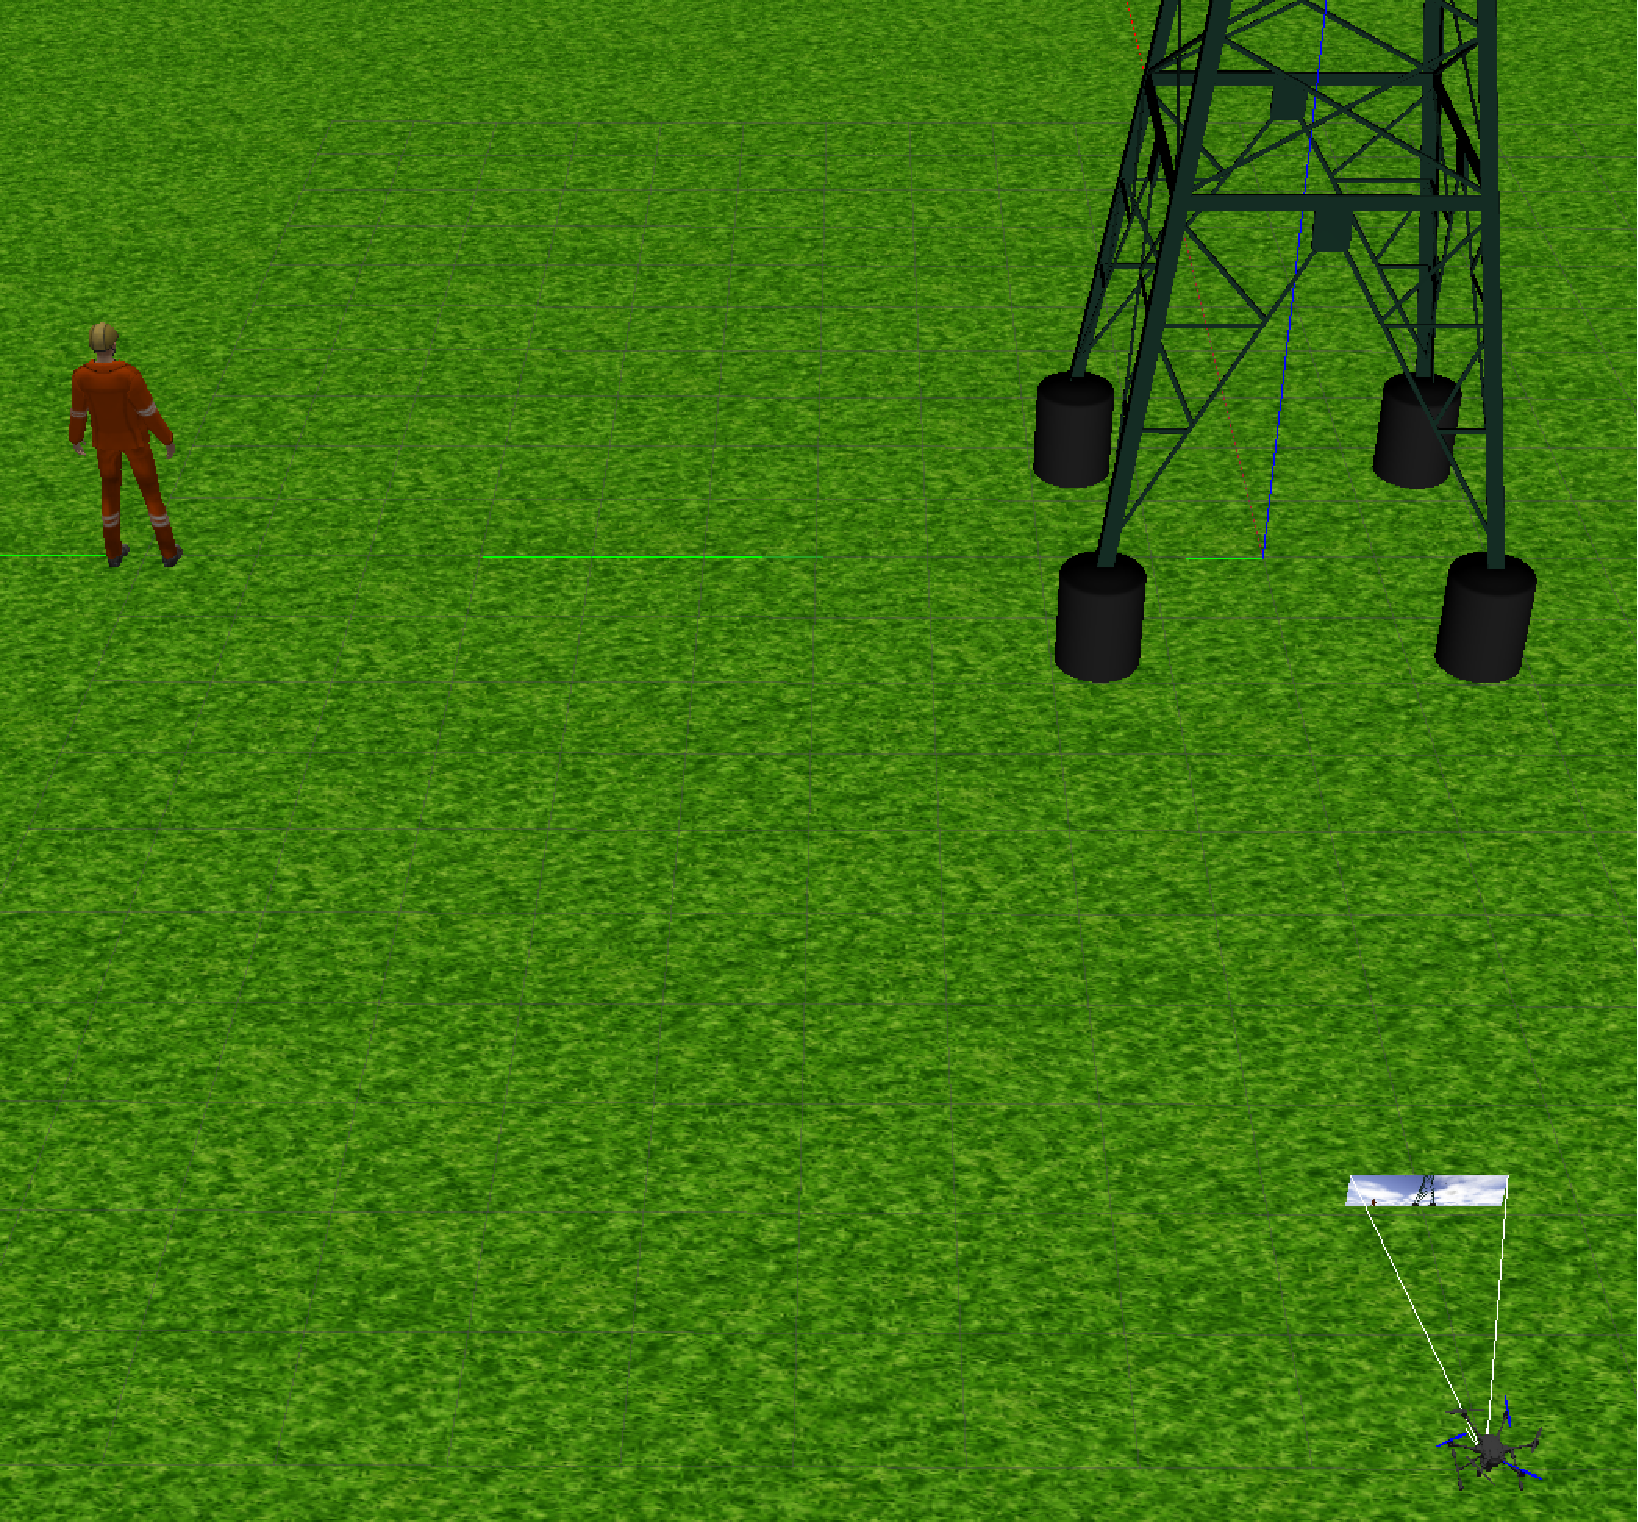
\includegraphics[width=.45\linewidth]{Results/figures/GazeboBatSta.pdf}}
    \hfill
    \subfloat[\gls{BT}'s starting status displayed with Groot]{
        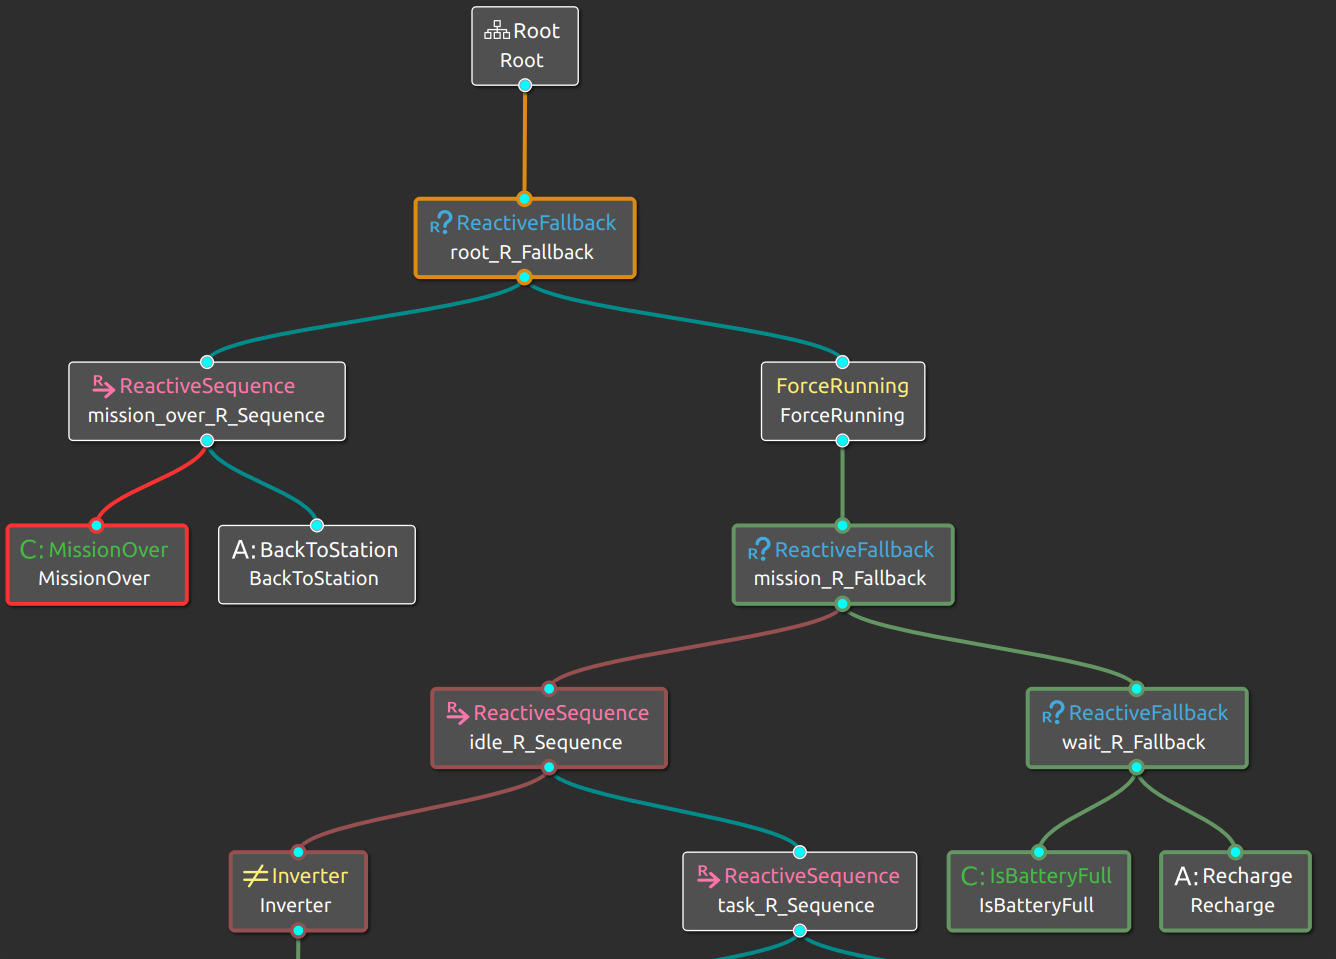
\includegraphics[width=.45\linewidth]{Results/figures/BTini.jpeg}}
    \caption{Initial status of the simulation: battery charged and no task queued.}
    \label{fig:BTinitialization}
\end{figure}

At the beginning, the \gls{UAV} has the battery charged, is landed on the charging station and has no task queued, then the \gls{BT} is returning \emph{SUCCESS} except for the \emph{Force Running} node, which keeps the \gls{BT} running by always returning \emph{RUNNING} (see Fig. \ref{fig:BTinitialization}). Note that Groot uses its own colour code to represent the result of each node in the previous tick. \emph{Green} stands for \emph{SUCCESS}, \emph{Red} for \emph{FAILURE}, \emph{Orange} for \emph{RUNNING} and \emph{White} for \emph{IDLE}. In addition, when a node is still called by a \emph{Reactive Control} node after it has finished, if the result is the same, the colour of the node is maintained but in a less intense tone. 

\begin{figure}[htbp]
    \centering
    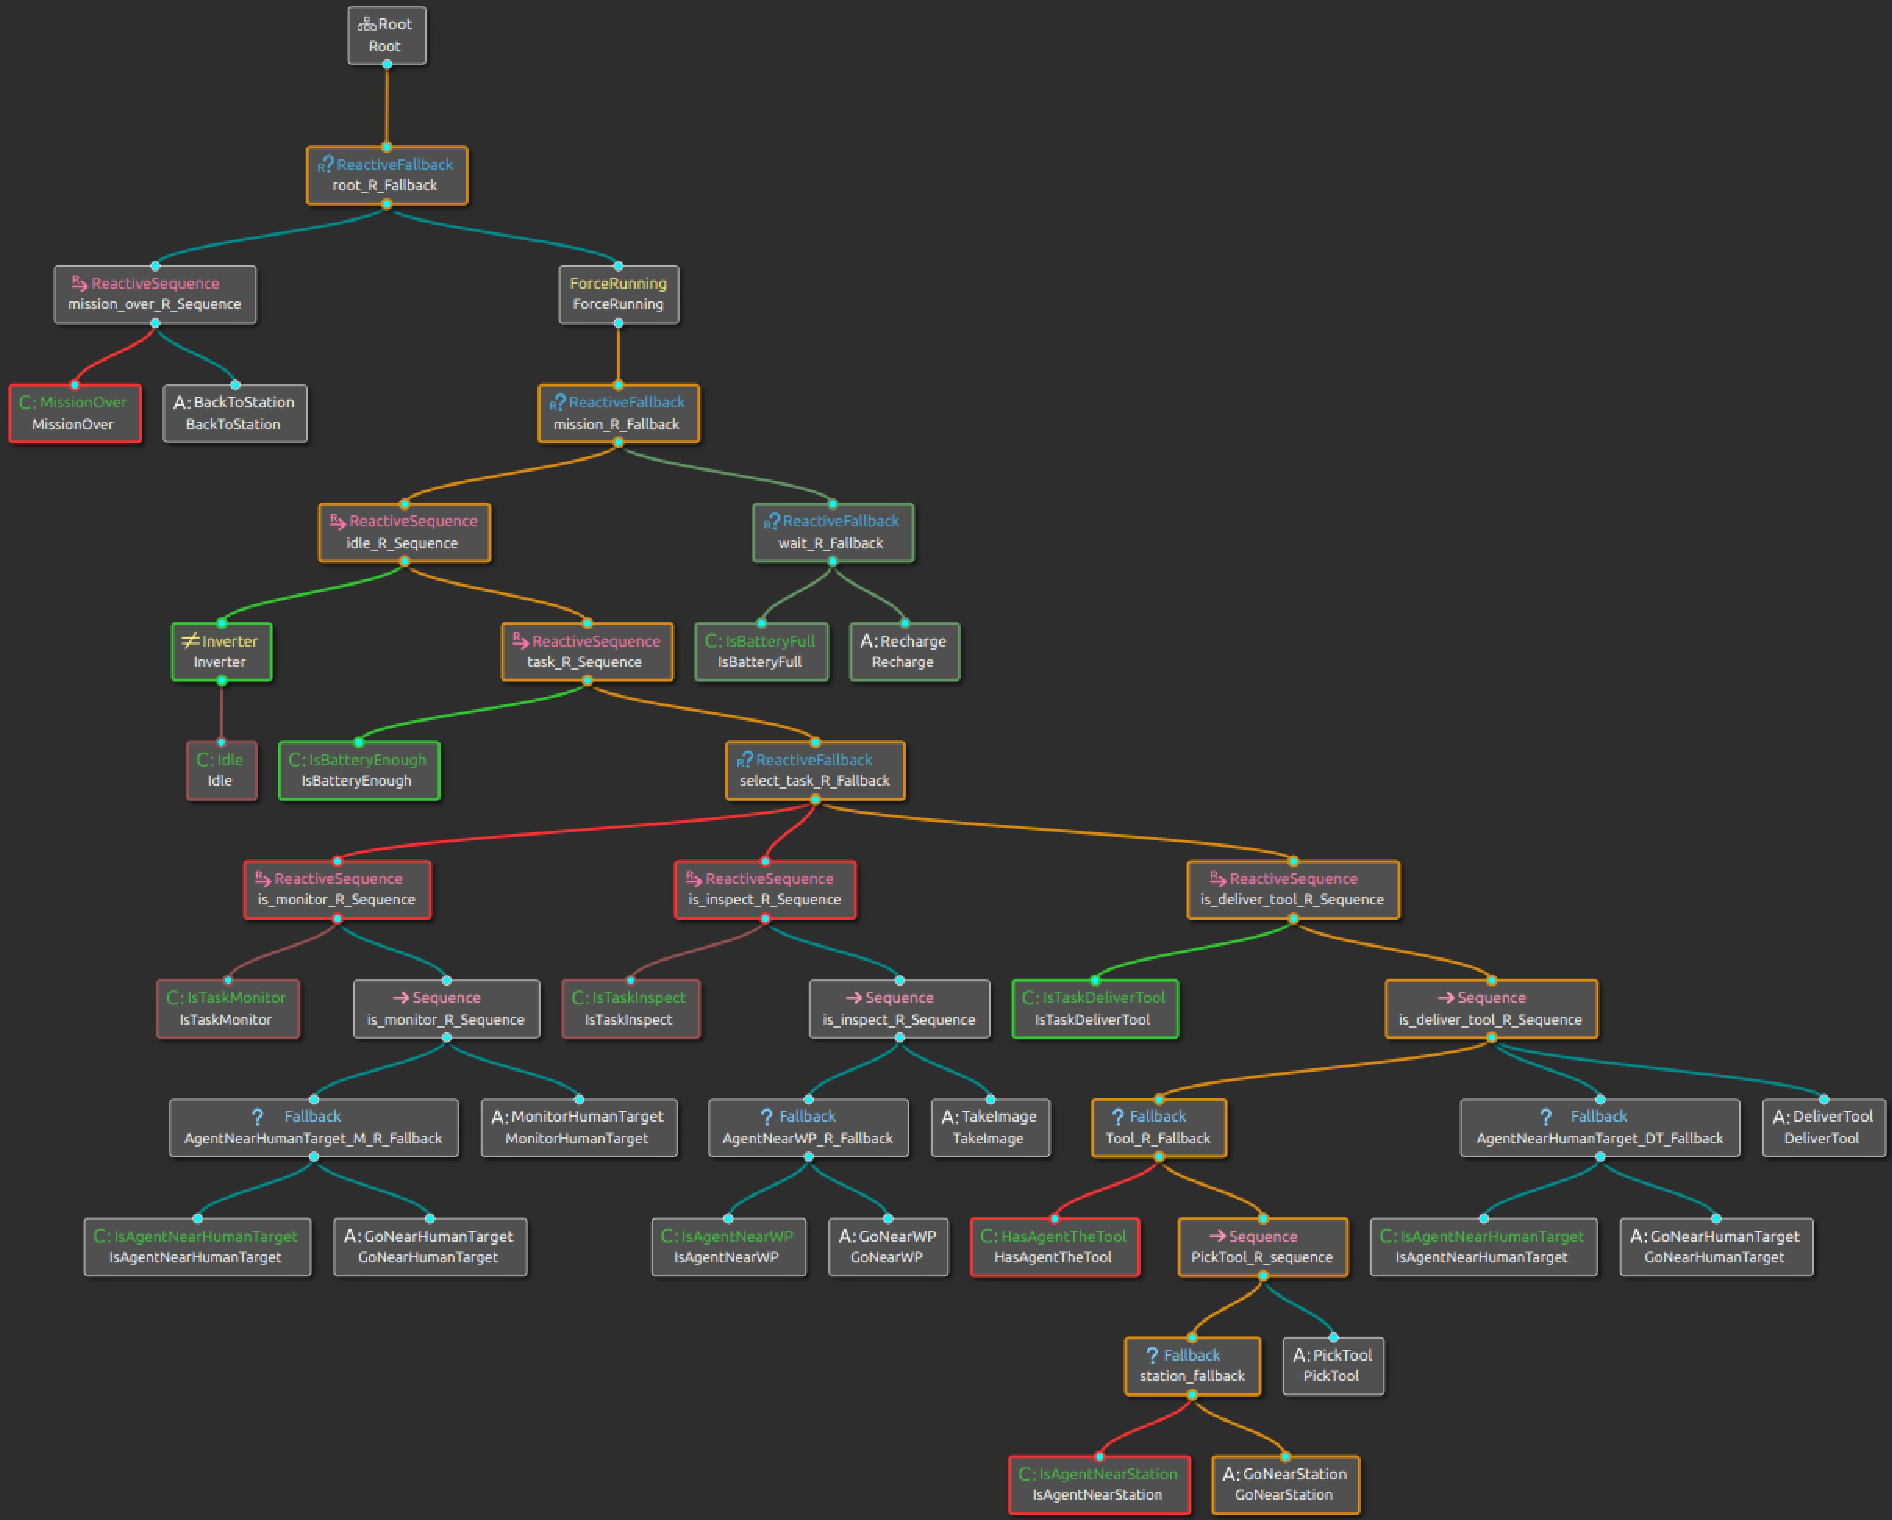
\includegraphics[width=.75\linewidth]{Results/figures/BTnoIdle.pdf}
    \caption{\gls{BT} transition from idle to \emph{Tool Delivery Task Tree}}
    \label{fig:NoIdle_DeliverToolTaskTree}
\end{figure}

For this simulation, tasks were requested from the \emph{High-Level Planner} before communication with the \emph{Agent Behaviour Manager} was established. Once the distributed block had finished initialising, communication between the two blocks could be established and with it the first task planning. While this happened, the \gls{BT} controlling the \gls{ACW} started executing and, not yet having any tasks assigned to it, directed the \gls{UAV} towards the charging station while it waited. Once the first task queue was communicated, the \gls{BT} checked which task was the first one and proceeded to execute it (see Fig. \ref{fig:NoIdle_DeliverToolTaskTree}). The code \ref{exit:newtaskqueue} shows the feedback posted by both blocks until the completion of the execution of the first task.

\begin{lstlisting}[caption={Feedback of the task planning process and communications between \emph{High-Level Planner} and \emph{Agent Behaviour Manager}at the beginning of the simulation}, breaklines=true, label=exit:newtaskqueue]
    [ INFO][/task_planner]: [Planner] Initialization complete

    [ INFO][/task_planner]: [incomingTask] Received a New Tasks:
        task_1: Deliver
            Tool: hammer (1.5kg): -2, 5, 0.9
            Human Target: human_target_1: 0, 10, 1.85
        task_2: Inspect
            Positions: (0, 0, 2) (10, 10, 2) (0, 10, 2) (10, 0, 2)
            Agent List:
        task_3: Monitor (1.5, 4)
            Human Target: human_target_1: 0, 10, 1.85
            Agent List:
    
    [ INFO][/task_planner]: [incomingTask] Allocating tasks...
    [ WARN][/task_planner]: [performTaskAllocation] No Agents connected yet. 3 pending tasks
    
    
    
    [ INFO][/uav_1/agent]: [AgentNode] uav_1 initialized. State: 0
    [ INFO][/uav_1/agent]: [Recharge] Calling take_off
    [ INFO][/uav_1/agent]: [Recharge] Moving to recharging station
    [ INFO][/uav_1/agent]: [Recharge] Calling land
    [ INFO][/uav_1/agent]: [Recharge] Charging...
    
    [ INFO][/task_planner]: [beaconCallback] New Agent connected: uav_1
    [ INFO][/task_planner]: [performTaskAllocation] Tasks Allocated:
    [ INFO][/task_planner]: [performTaskAllocation] Agent id: uav_1
        Agent type: PhysicalACW
        Task list: (3 tasks)
            task_1: DeliverTool
            task_2: Inspect
            task_3: Monitor
    
    [ INFO][/uav_1/agent]: [newTaskList] Received a NewTaskList Action
    [ INFO][/uav_1/agent]: task_1: DeliverTool
    [ INFO][/uav_1/agent]: [Recharge] halt requested
    [ INFO][/uav_1/agent]: [GoNearStation] Moving near Tool...
\end{lstlisting}

The \emph{Tool Delivery Task Tree} functioned perfectly well. In Gazebo, the movement of the \gls{ACW} from one side to the other was observed as the \gls{BT} traversed the nodes of the subtree of this task (see Fig. \ref{fig:Gazebo_DeliverTree}). In addition, the task result was checked for correct communication with the centralised block, which used the moment to re-evaluate the plan to see if it is still within the optimal plan (see code \ref{exit:tasksFInishAndReplanning}). As the plan did not change, the \gls{BT} continued to execute the queued tasks. As it has already been shown that the activation of \emph{Action} nodes in the \gls{BT} correctly moves the \gls{ACW} in the Gazebo simulation, no screenshots of the simulation are shown from now on as they are not relevant. Figure \ref{fig:Gazebo_InspectTree} shows the evolution of the \gls{BT} during the execution of the \emph{Inspection} task, for which the \gls{BT} also proved to work perfectly. 

\begin{figure}[htbp]
    \centering
    \subfloat[Initial position: charge station]{
        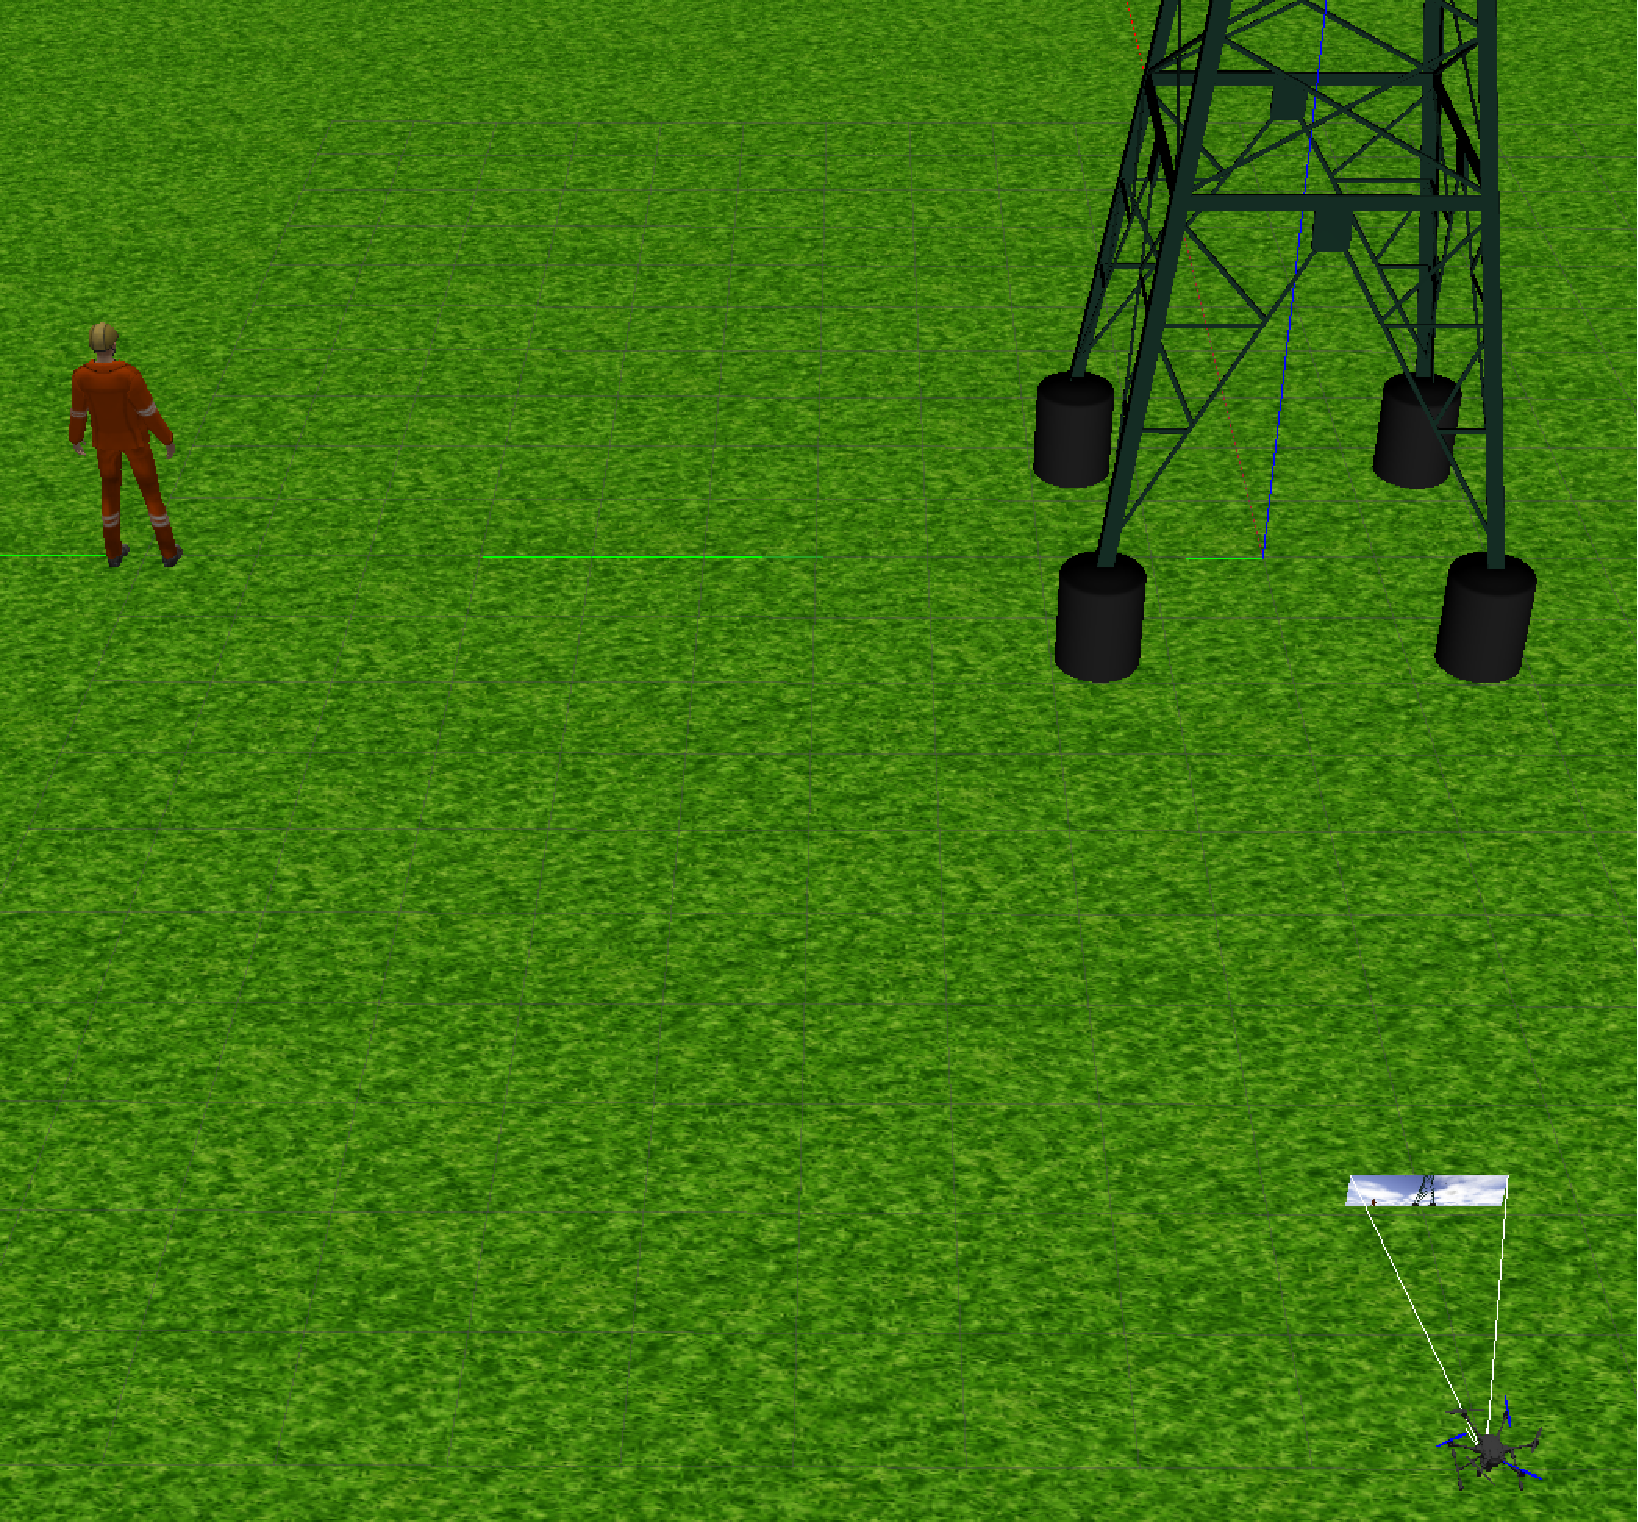
\includegraphics[width=.3\linewidth]{Results/figures/GazeboBatSta.pdf}}
    \hfill
    \subfloat[Base station: tool picking]{
        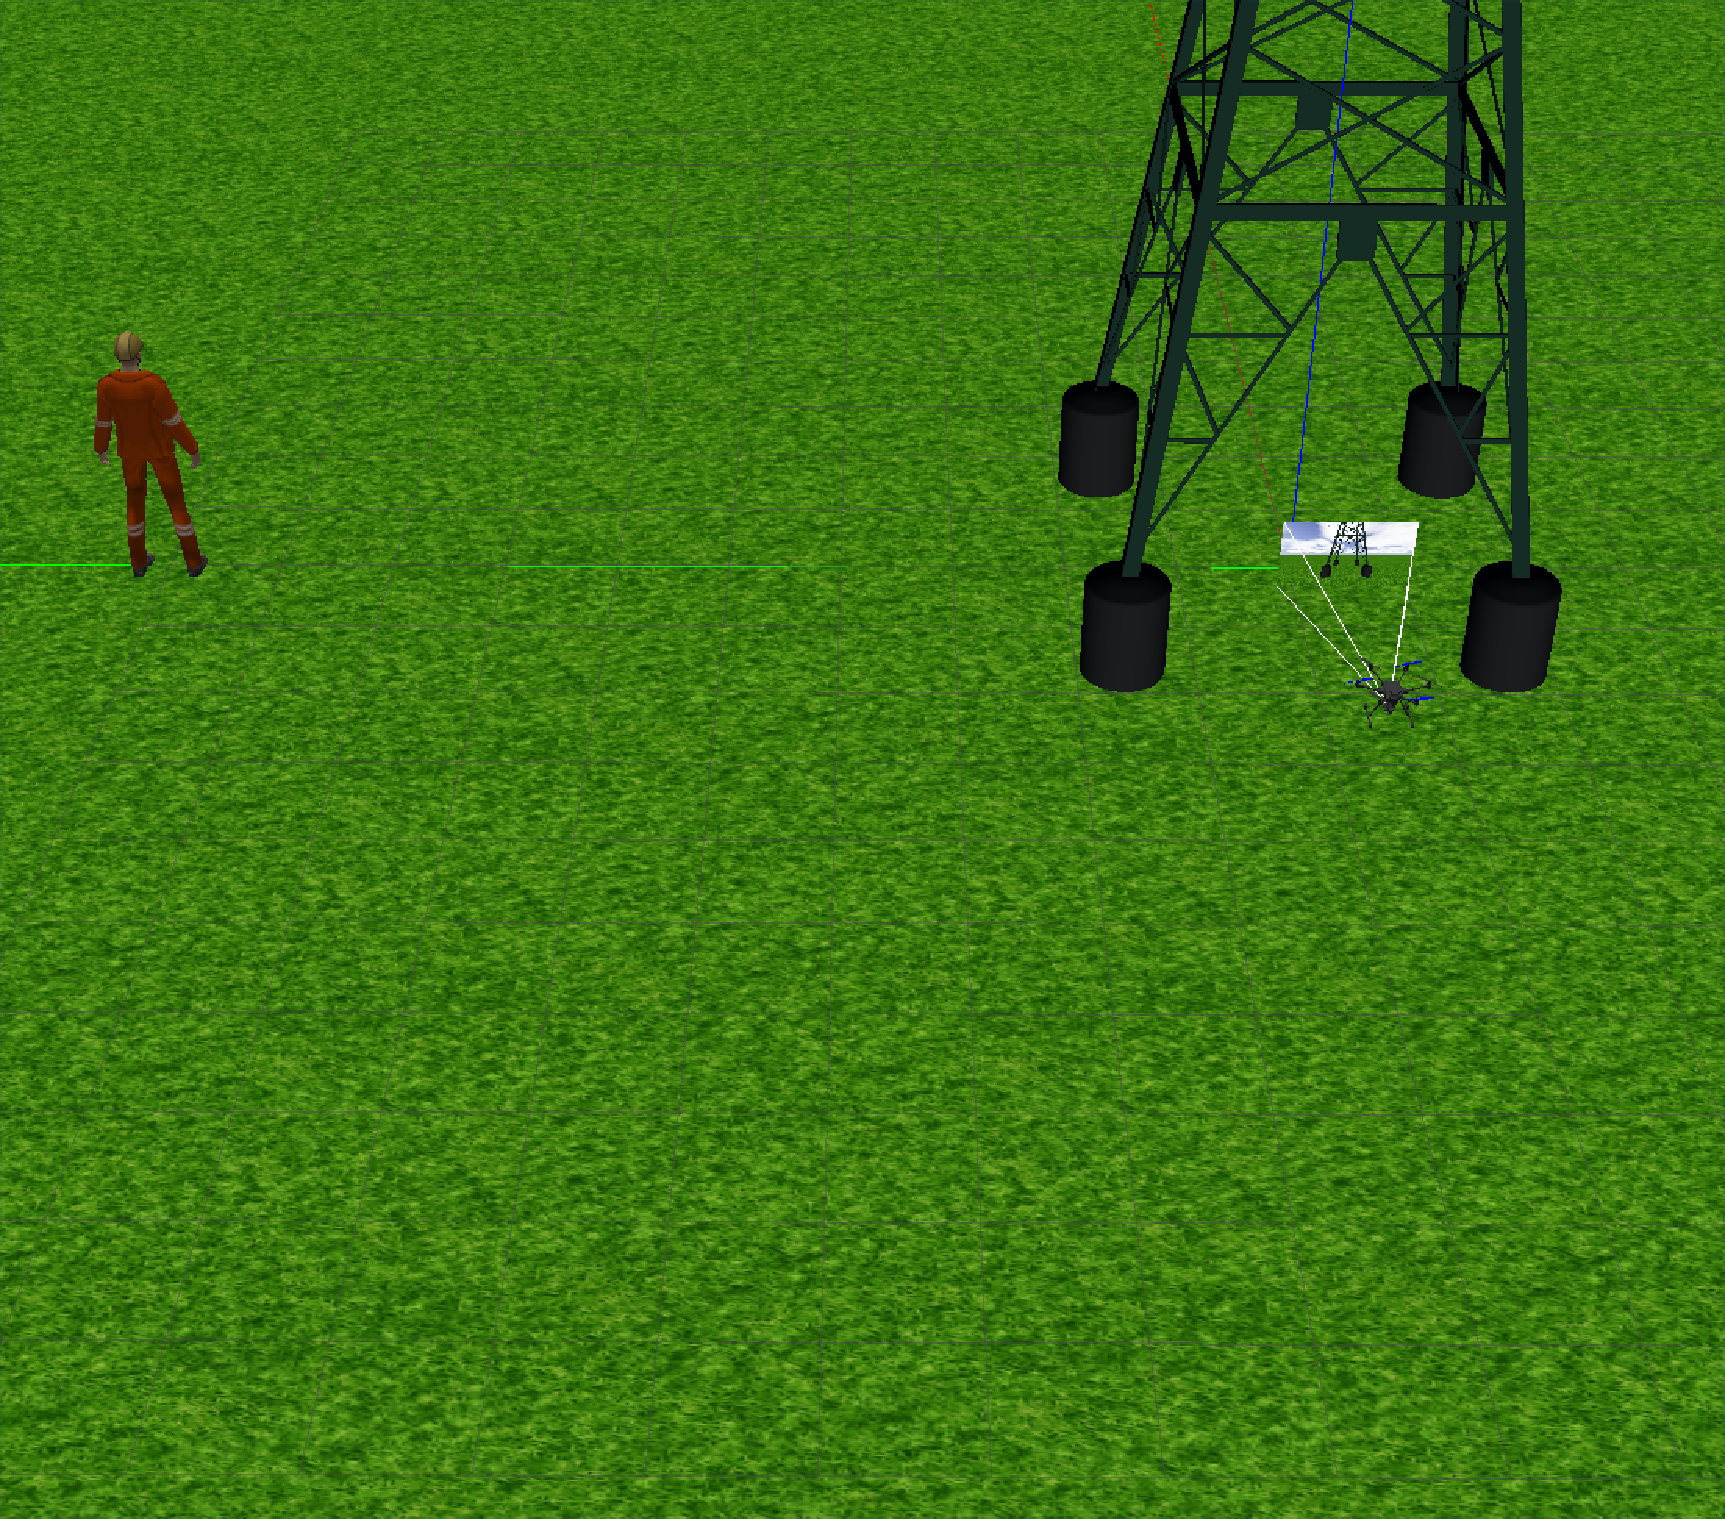
\includegraphics[width=.3\linewidth]{Results/figures/GazeboTool.pdf}}
    \hfill
    \subfloat[Human target position: tool delivery]{
        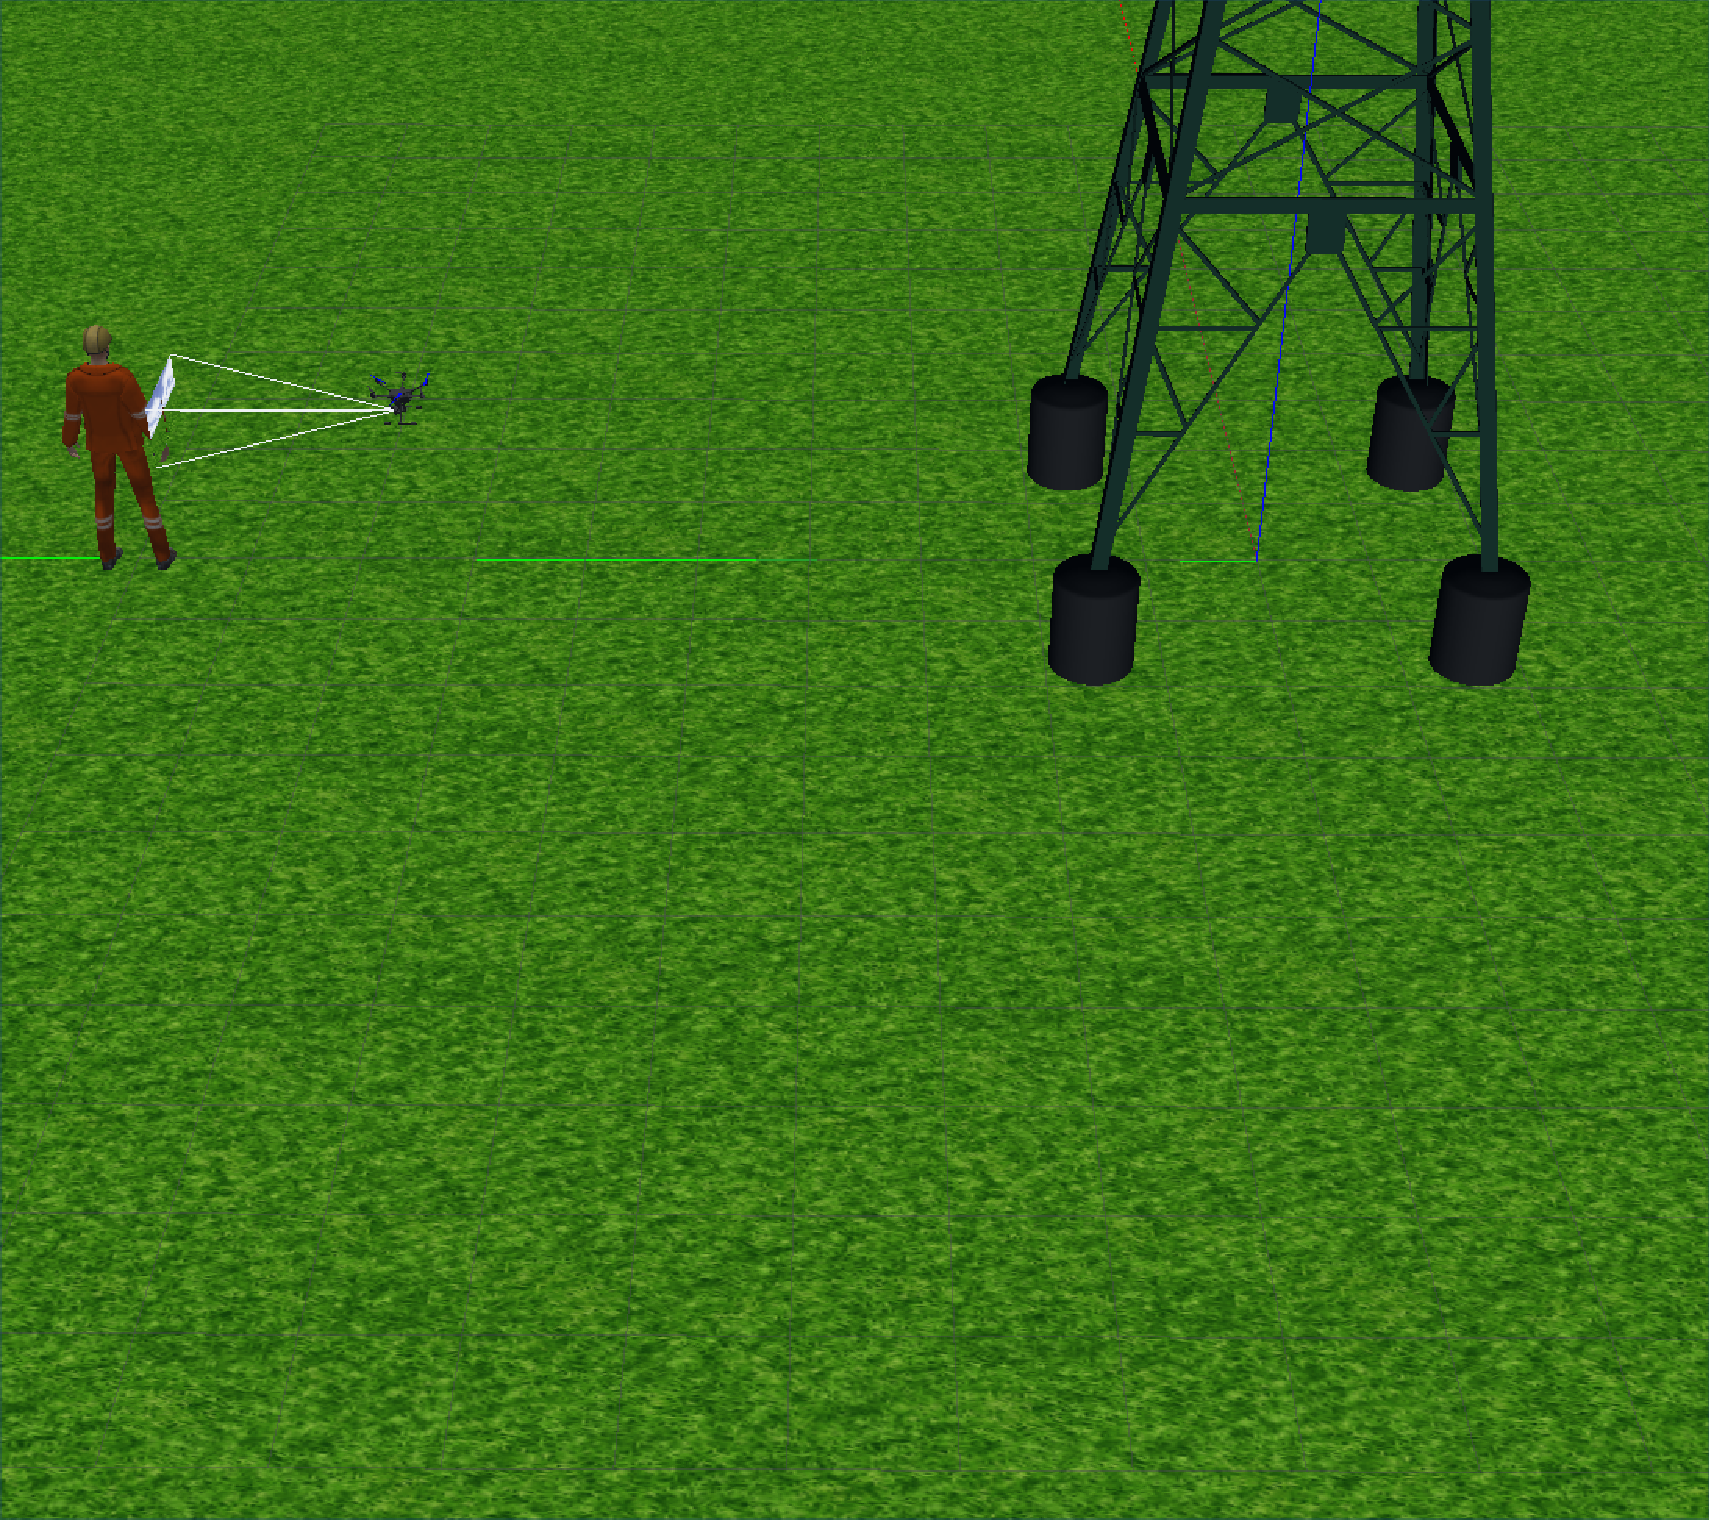
\includegraphics[width=.3\linewidth]{Results/figures/GazeboHuman.pdf}}
    \hfill
    \\
    \subfloat[Activation of \emph{Go Near Station} action after checking \emph{Has ACW the tool?} and \emph{Is ACW near Station?} conditions]{
        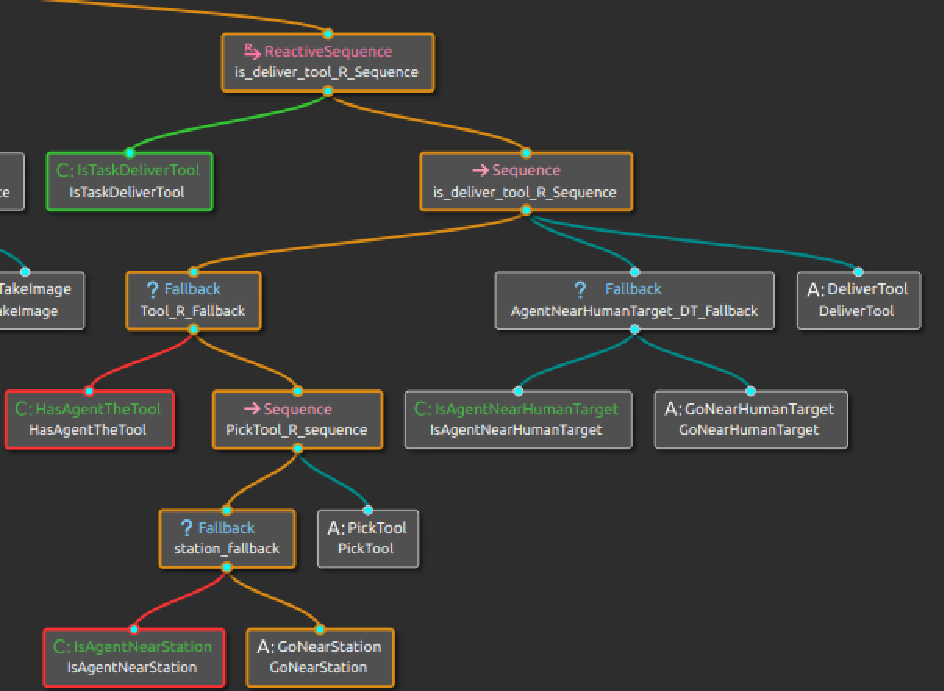
\includegraphics[width=.45\linewidth]{Results/figures/BTDTGNS.pdf}}
    \hfill
    \subfloat[Activation of \emph{Pick Tool} action after arriving at the base station]{
        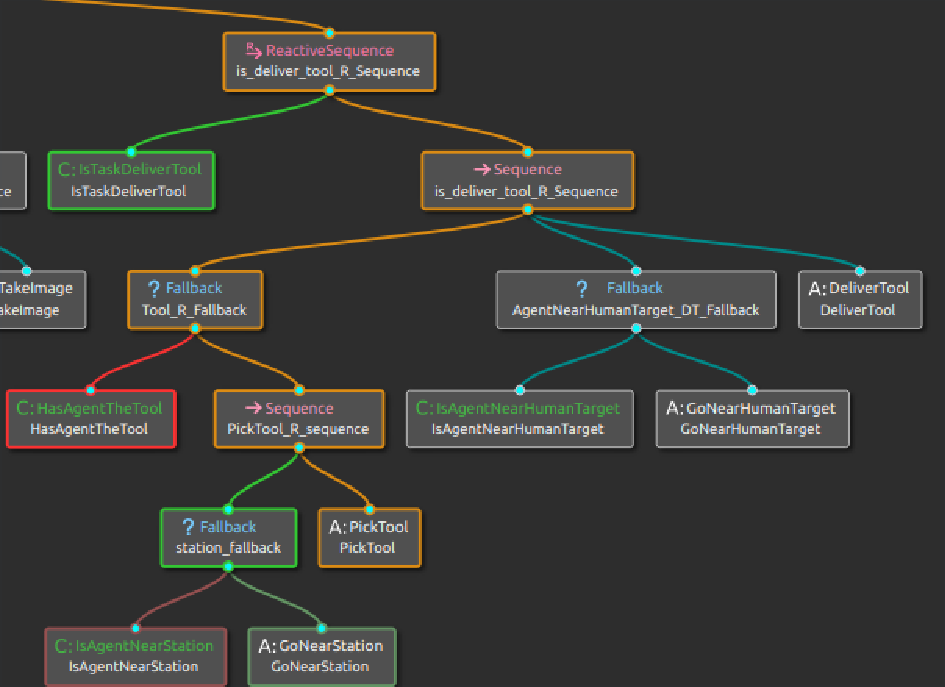
\includegraphics[width=.45\linewidth]{Results/figures/BTDTPT.pdf}}
    \\
    \subfloat[Activation of \emph{Go Near Human Target} action after having the tool and checking \emph{Is ACW Human Target?} condition]{ 
        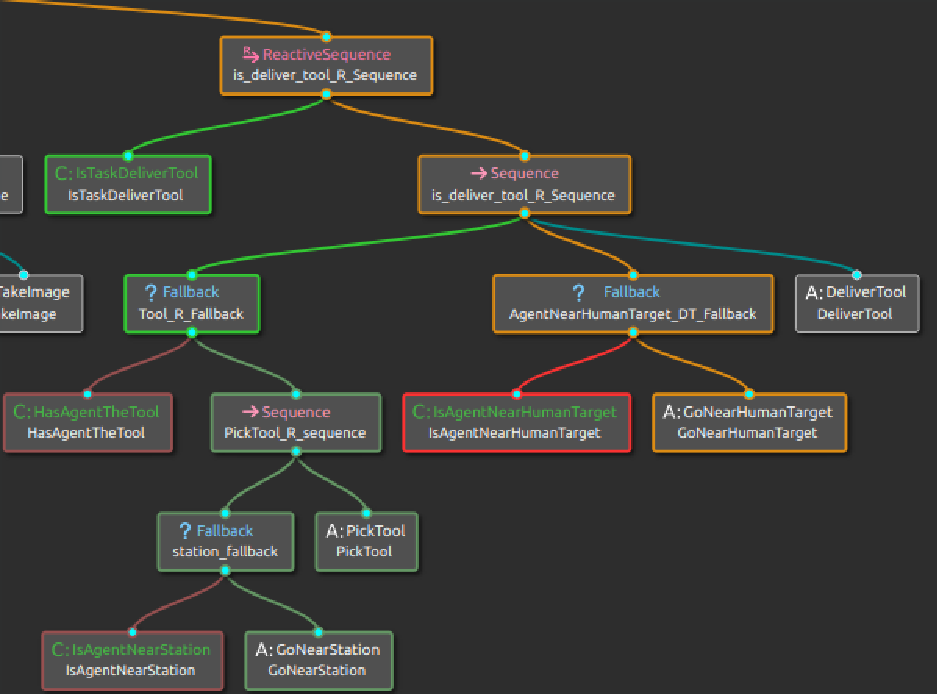
\includegraphics[width=.45\linewidth]{Results/figures/BTDTGNHT.pdf}}
    \hfill
    \subfloat[Activation of \emph{Deliver Tool} action after arriving near human target having the tool]{
        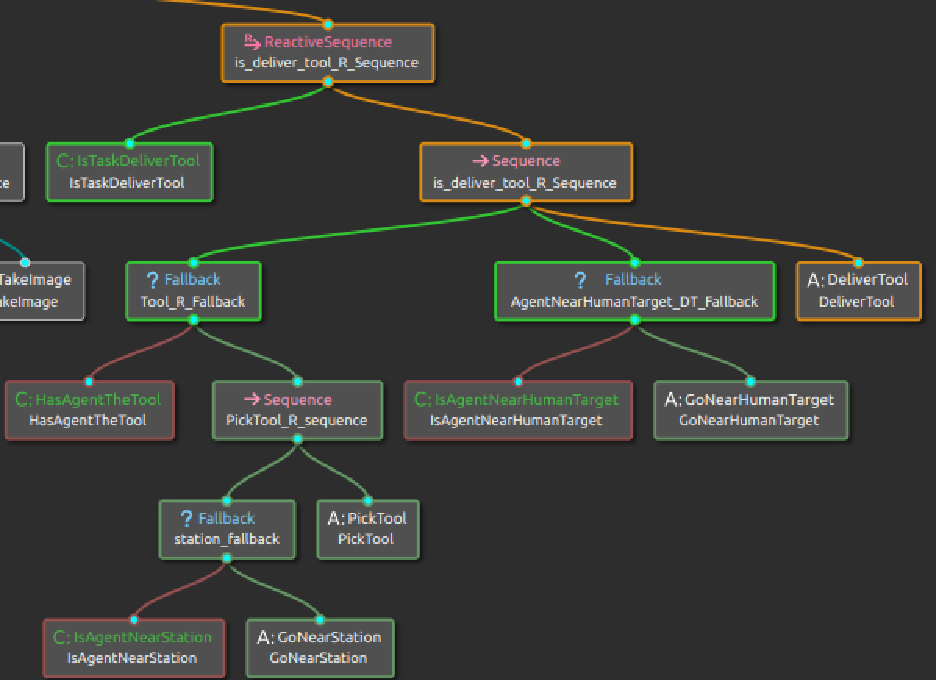
\includegraphics[width=.45\linewidth]{Results/figures/BTDTDT.pdf}}
    \caption{Evolution of the simulation during the execution of the \emph{Tool Delivery Task Tree}}
    \label{fig:Gazebo_DeliverTree}
\end{figure}

\begin{figure}[htbp]
    \centering
    \subfloat[Activation of \emph{Go Near WP} action after checking \emph{Is Agent Near WP?} condition]{
        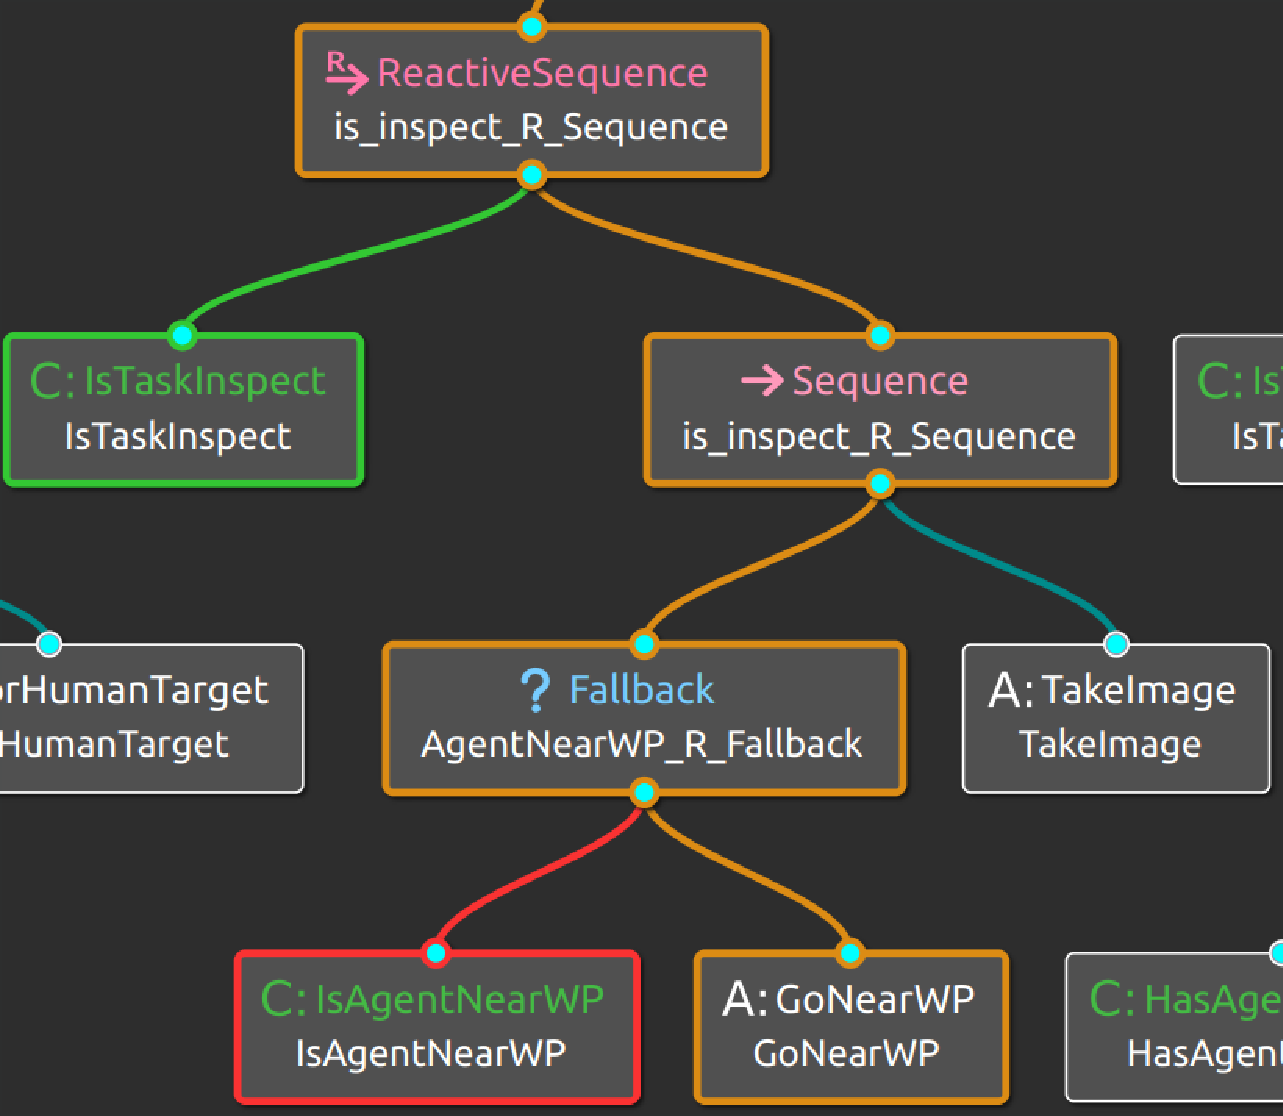
\includegraphics[width=.45\linewidth]{Results/figures/BTIGNWP.pdf}}
    \hfill
    \subfloat[Activation of \emph{Take Image} action after arriving near WP]{
        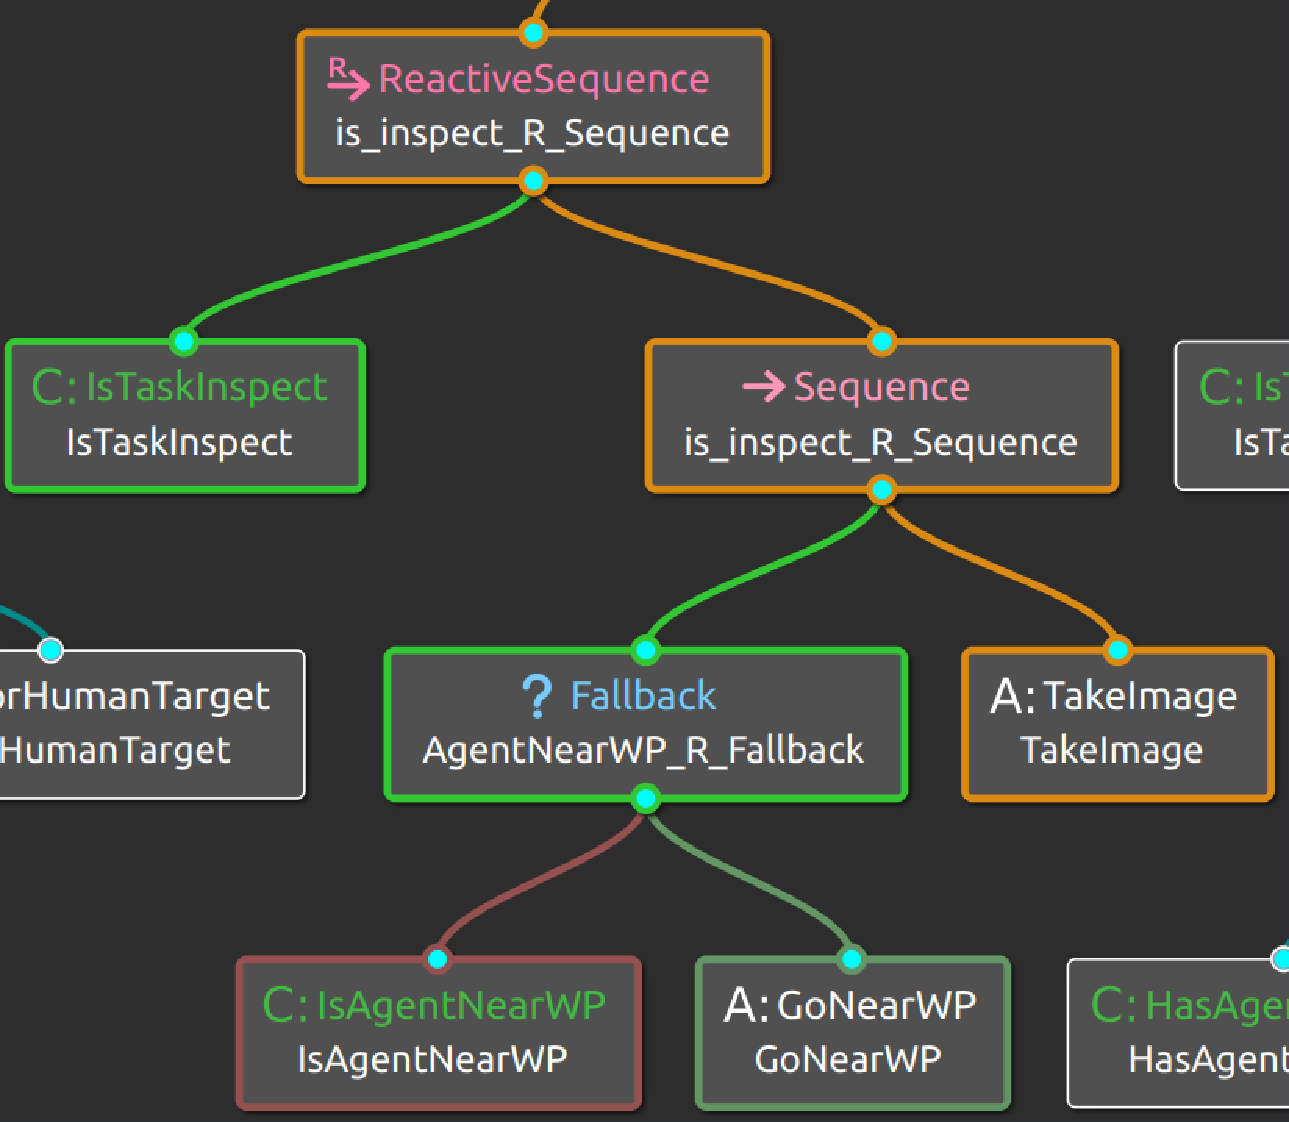
\includegraphics[width=.45\linewidth]{Results/figures/BTITI.pdf}}
    \caption{Evolution of the \gls{BT} during the execution of the \emph{Inspection Task Tree}}
    \label{fig:Gazebo_InspectTree}
\end{figure}

\begin{lstlisting}[caption={Feedback messages printed out during replanning that were carried out when tasks were completed}, breaklines=true, label=exit:tasksFInishAndReplanning]
    [ INFO][/task_planner]: [taskResultCB] (uav_1) task_1(DeliverTool) SUCCEEDED. Reallocating just in case...
    [ INFO][/task_planner]: [performTaskAllocation] Tasks Allocated:
    [ INFO][/task_planner]: [performTaskAllocation] Agent id: uav_1
        Agent type: PhysicalACW
        Task list: (2 tasks)
            task_2: Inspect
            task_3: Monitor
    
    [ INFO][/task_planner]: [taskResultCB] (uav_1) task_2(Inspect) SUCCEEDED. Reallocating just in case...
    [ INFO][/task_planner]: [performTaskAllocation] Tasks Allocated:
    [ INFO][/task_planner]: [performTaskAllocation] Agent id: uav_1
        Agent type: PhysicalACW
        Task list: (1 tasks)
            task_3: Monitor
\end{lstlisting}

Finally, when this task was finished, the \gls{BT} proceeded to execute the \emph{Safety Monitoring} task, which was also carried out without problems (see Fig. \ref{fig:Gazebo_MonitorTree}). Code \ref{exit:firstPlanFeedback} shows all feedback messages printed by the \emph{Agent Behaviour Manager} during the execution of the whole plan. 

\begin{figure}[htbp]
    \centering
    \subfloat[Activation of \emph{Go Near Human Target} action after checking \emph{Is Agent Near Human Target?} condition]{
        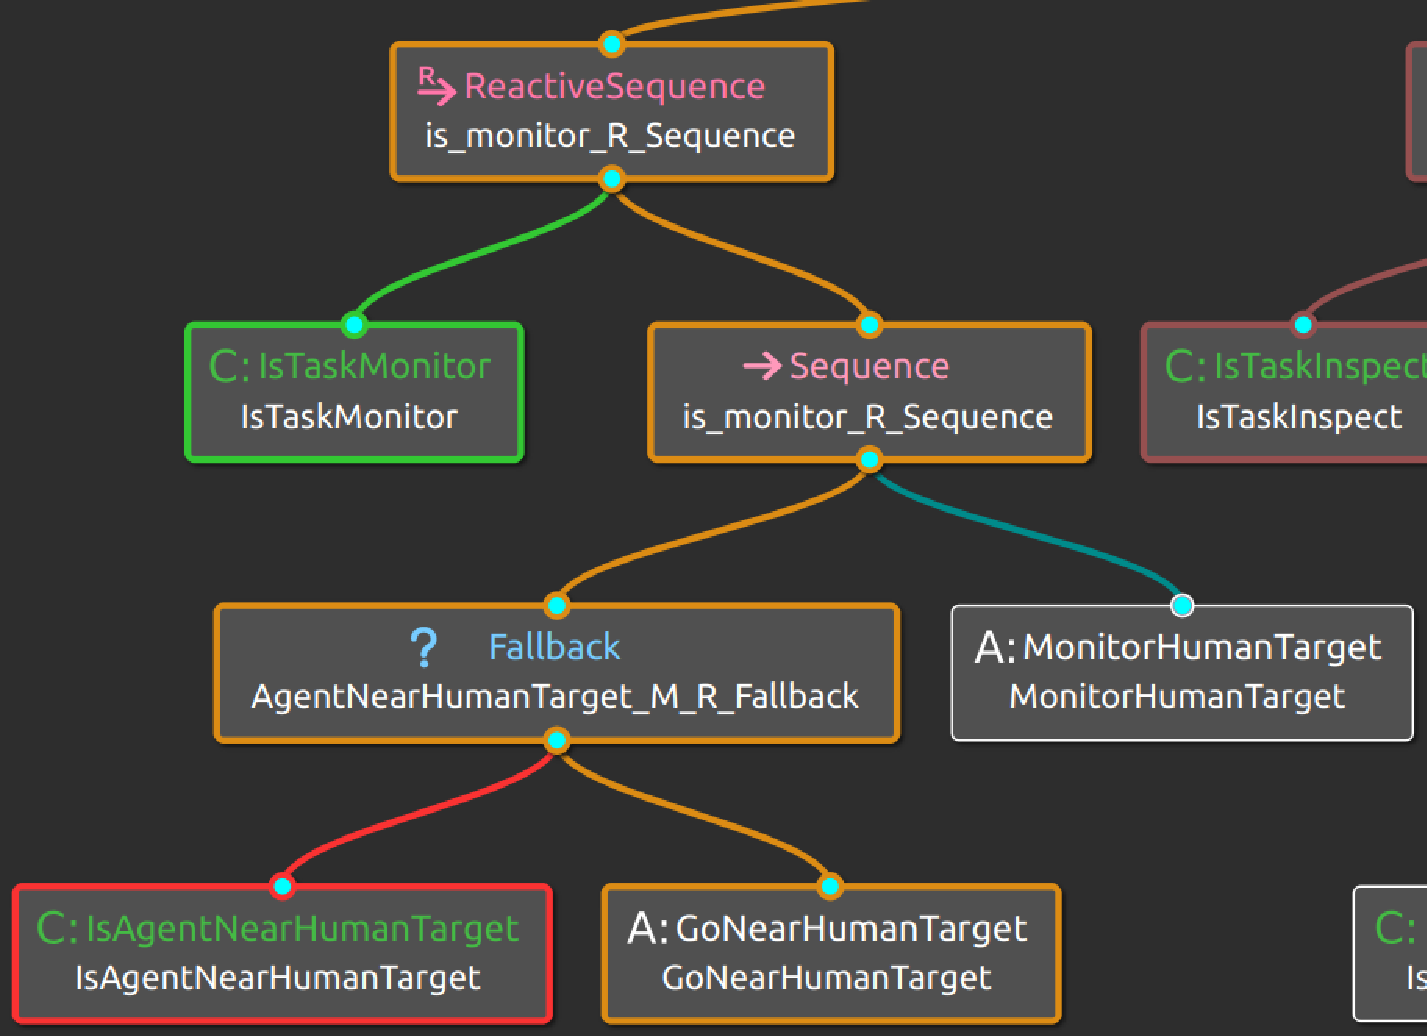
\includegraphics[width=.45\linewidth]{Results/figures/BTMGNHT.pdf}}
    \hfill
    \subfloat[Activation of \emph{Monitor Human Target} action after arriving near Human Target]{
        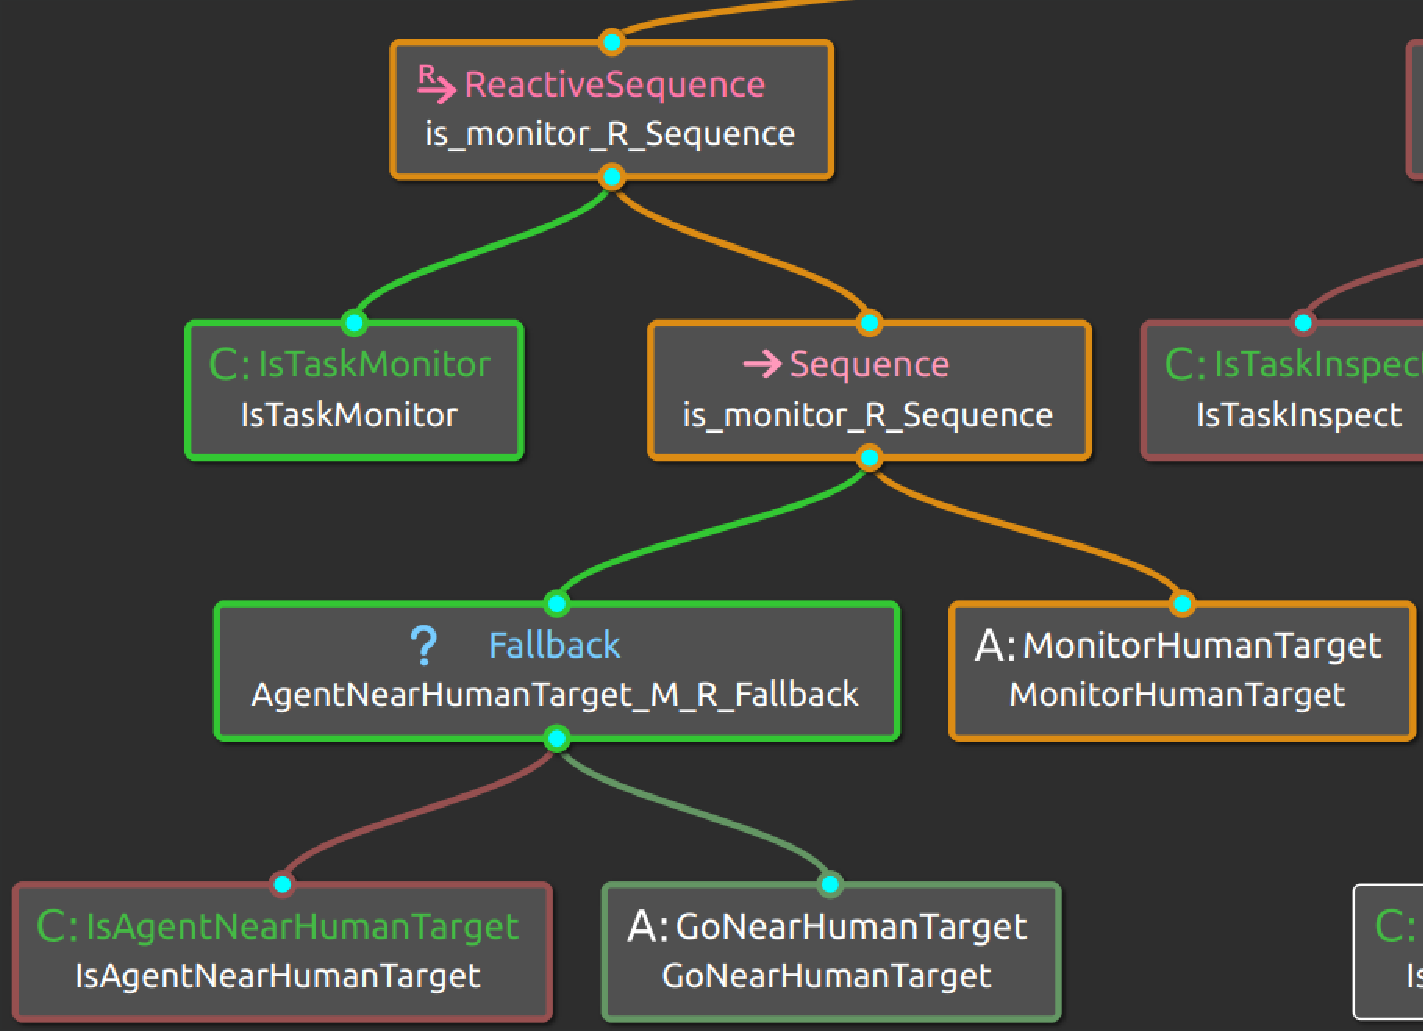
\includegraphics[width=.45\linewidth]{Results/figures/BTMMHT.pdf}}
    \caption{Evolution of the \gls{BT} during the execution of the \emph{Monitoring Task Tree}}
    \label{fig:Gazebo_MonitorTree}
\end{figure}

\begin{lstlisting}[caption={Feedback messages printed by the \emph{Agent Behaviour Manager} during the execution of the whole plan}, breaklines=true, label=exit:firstPlanFeedback]
    [ INFO][/uav_1/agent]: [newTaskList] Received a NewTaskList Action
    [ INFO][/uav_1/agent]: task_1: DeliverTool
    [ INFO][/uav_1/agent]: [Recharge] halt requested
    [ INFO][/uav_1/agent]: [GoNearStation] Moving near Tool...
    [ INFO][/uav_1/agent]: [PickTool] Calling Lower-level controllers...
    [ INFO][/uav_1/agent]: [PickTool] PICK TOOL FINISHED
    [ INFO][/uav_1/agent]: [GoNearHumanTarget] Moving near HT...
    [ INFO][/uav_1/agent]: [DeliverTool] Calling Lower-level controllers...
    [ INFO][/uav_1/agent]: [DeliverTool] DELIVER TOOL TASK FINISHED (true)
    [ INFO][/uav_1/agent]: task_2: Inspect
    [ INFO][/uav_1/agent]: [GoNearWP] Moving near WP...
    [ INFO][/uav_1/agent]: [TakeImage] Calling Lower-level controllers...
    [ INFO][/uav_1/agent]: [TakeImage] INSPECT TASK FINISHED (true)
    [ INFO][/uav_1/agent]: task_3: Monitor
    [ INFO][/uav_1/agent]: [GoNearHumanTarget] Moving near HT...
    [ INFO][/uav_1/agent]: [MonitorHumanTarget] Calling Lower-level controllers...
\end{lstlisting}

\emph{Safety Monitoring} task ends when the operator requests it, so the fake block pretending to be the low-level controller for this task is programmed so that the task never ends. This task remains in the pending tasks queue until the mission is completed or it is overwritten by a task of another type with the same \gls{ID}, which is a contemplated case for which the planner is prepared and warns the operators that an unfinished task is going to be deleted. Since during planning, tasks are assigned in order, the non-completion of this task is not a problem for the execution of other tasks, but an opportunity to study in a controlled way the emergency protocols and the response of both blocks to different unforeseen events.

It should be noted that if at some point the \gls{ACW} completed all the pending tasks and became \emph{Idle} again, it would automatically go to the charging station to recharge the battery while waiting for a new task to arrive. To test how well this works, a simulation was performed in which a single \emph{Inspection} task was requested in order to wait for the \gls{UAV} to become \emph{Idle}. The result of this test can be seen in figure \ref{fig:chargeBecouseIdle}.

\begin{figure}[htbp]
    \centering
    \subfloat[\emph{Inspection} task is running]{
        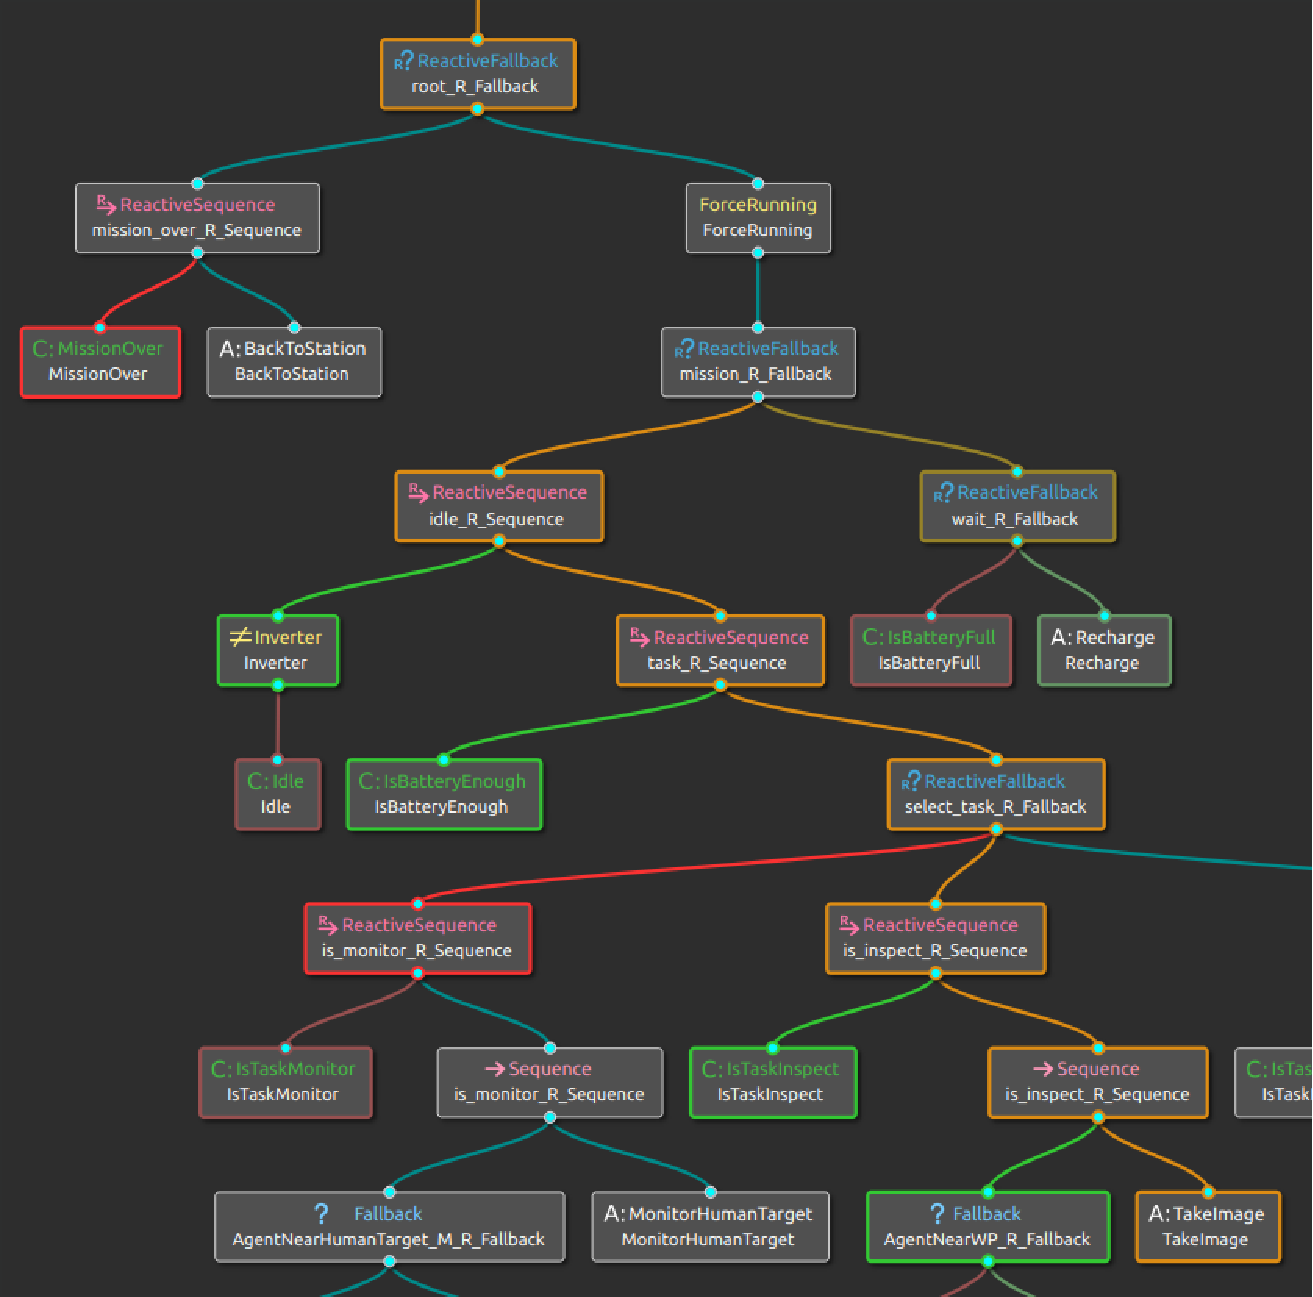
\includegraphics[width=.3\linewidth]{Results/figures/BTTaskRunnin.pdf}}
    \hfill
    \subfloat[\emph{Inspection} task finish and returs \emph{SUCCESS}]{
        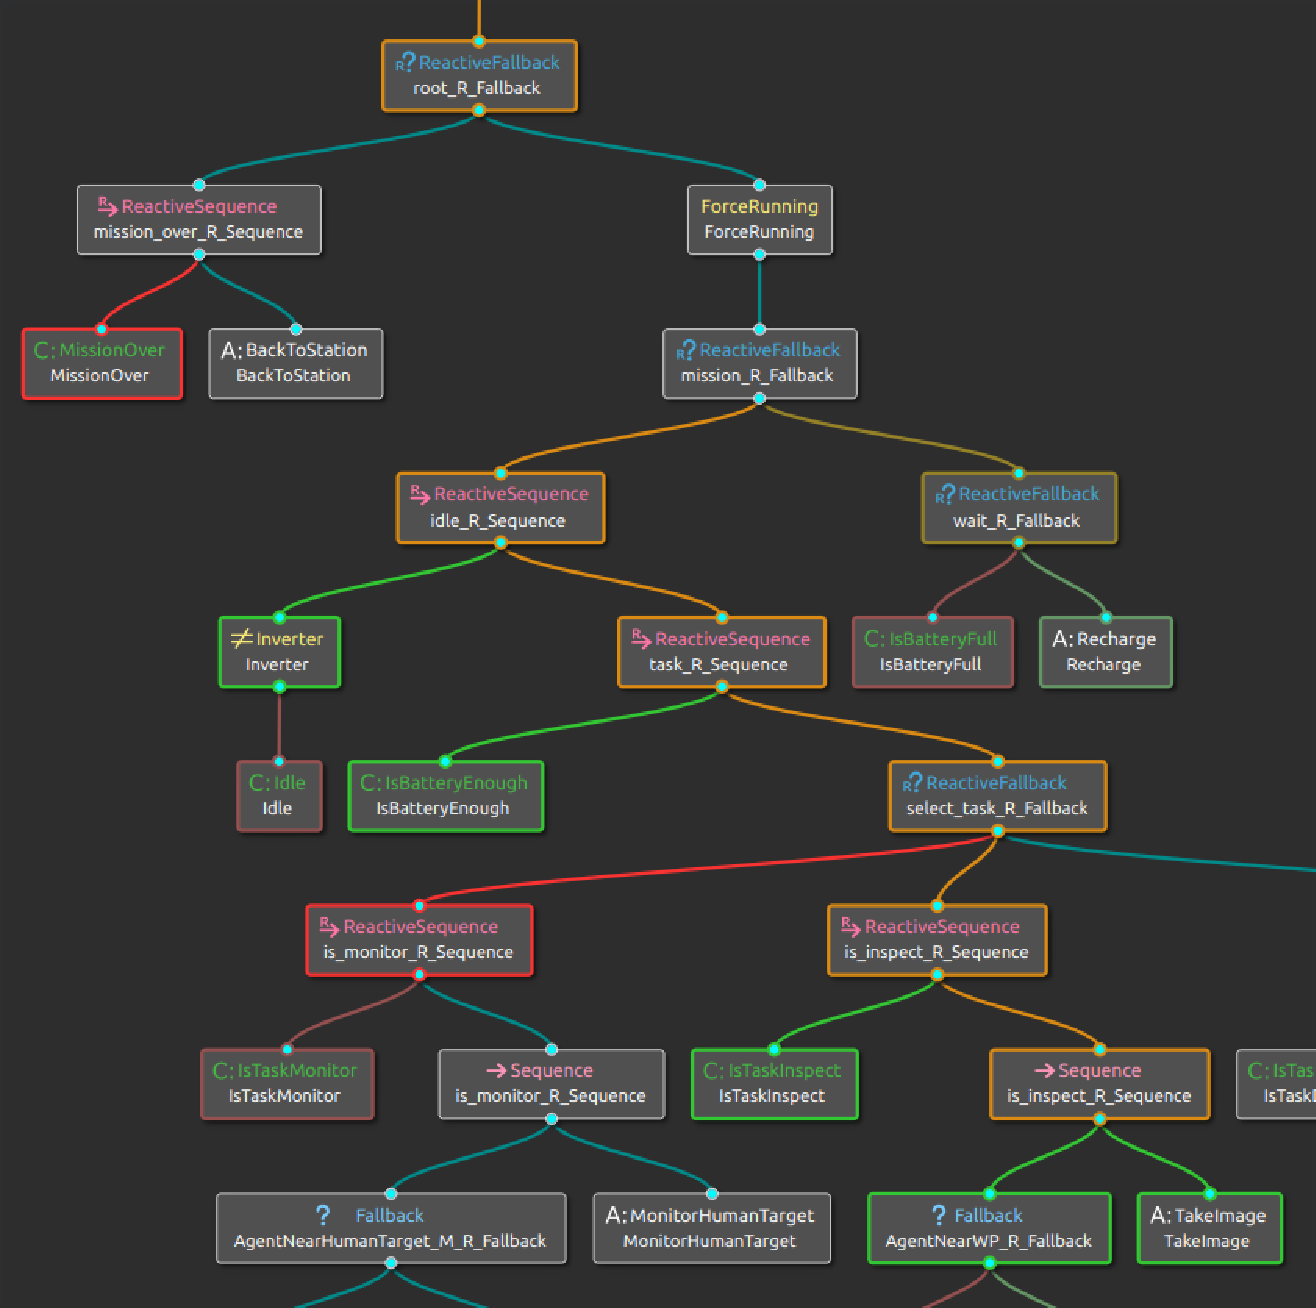
\includegraphics[width=.3\linewidth]{Results/figures/BTTaskSuccess.pdf}}
    \hfill
    \subfloat[As \gls{ACW} is now \emph{Idle}, \emph{Recharge} node is executed]{
        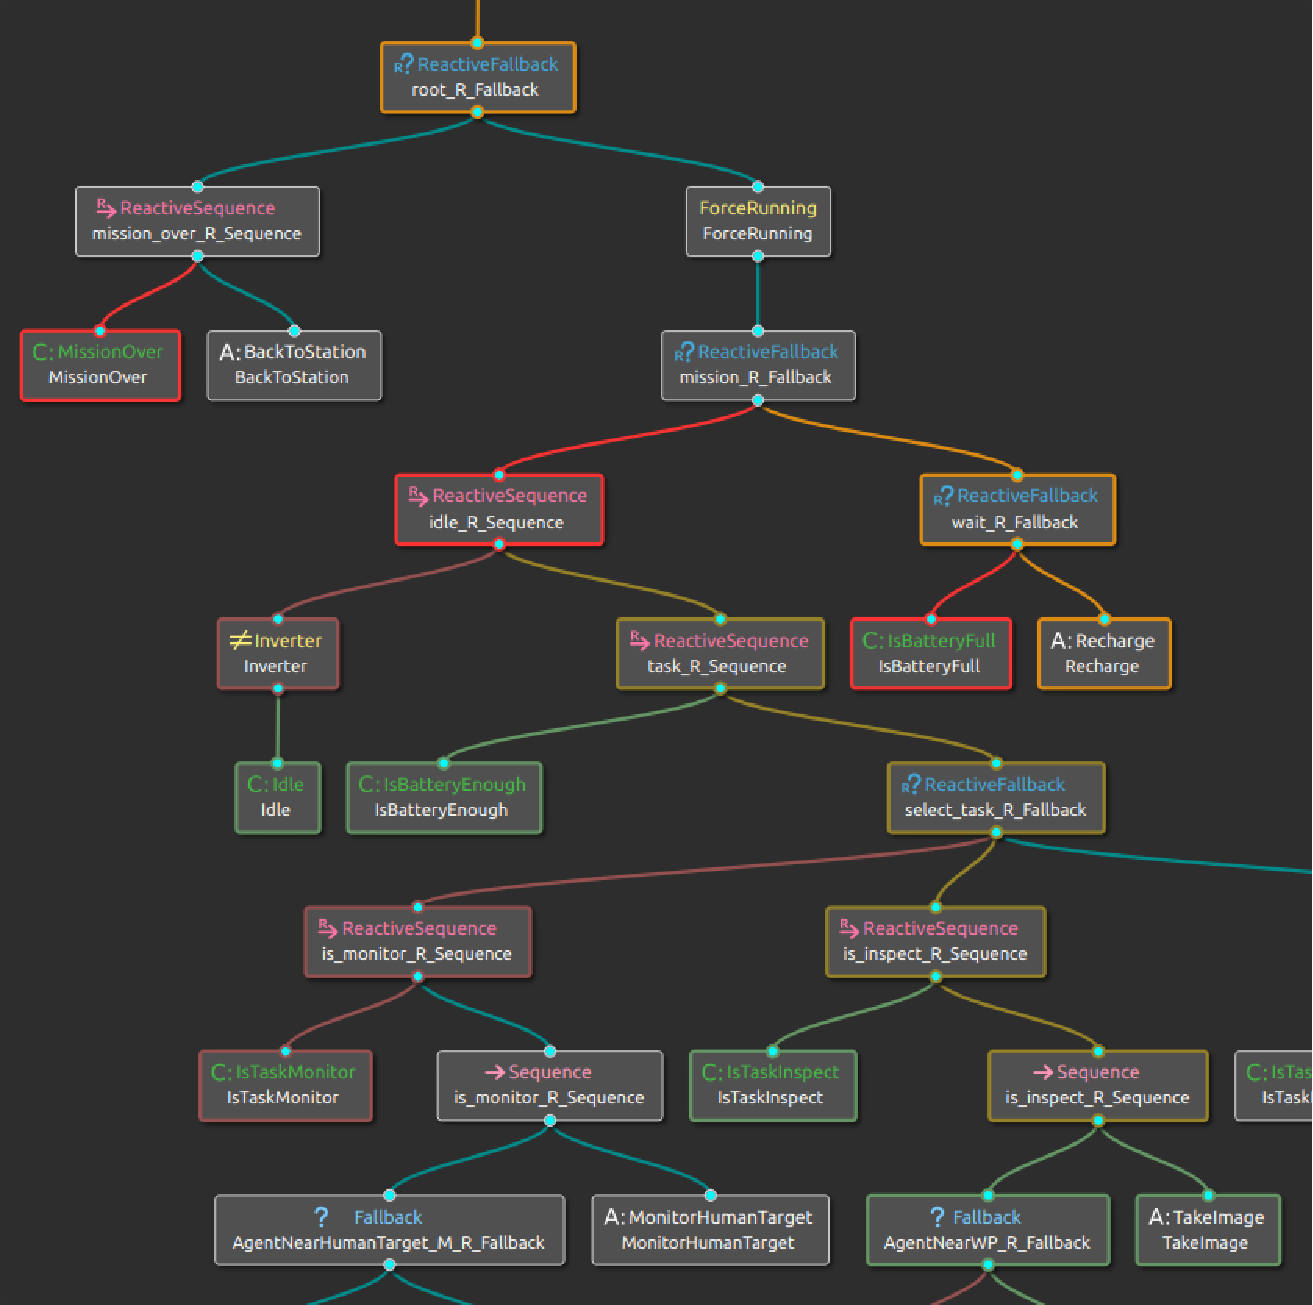
\includegraphics[width=.3\linewidth]{Results/figures/BTChargeBecIdle.pdf}}
    \caption{\gls{BT} leads the \gls{UAV} to the charging station after running out of assigned tasks}
    \label{fig:chargeBecouseIdle}
\end{figure}

Once it had been verified that the system worked well in the absence of unforeseen events, the system was tested in all kinds of situations. First, the \gls{BT}'s ability to stop the current task and switch to the execution of the new task in the event of a change of plans was tested. This was done by first requesting a \emph{Safety Monitoring} task and then requesting a \emph{Tool Delivery} task, which, having a higher priority, will move the previous task from the top of the queue. Both figure \ref{fig:event_ChangeOfPlans} and code \ref{exit:event_ChangeOfPlans} show how, after the replanning and the arrival of the new queue, the \gls{BT} stopped the task being executed by the \gls{ACW}, a \emph{Safety Monitoring} task in this case, and proceeded with the execution of the \emph{Tool Delivery} task, which now occupies the first place in the queue.

\begin{lstlisting}[caption={Feedback messages printed after a change of plans. \emph{Tool Delivery} task displaces \emph{Safety Monitoring} task}, breaklines=true, label=exit:event_ChangeOfPlans]
    [ INFO][/task_planner]: [incomingTask] Received a New Task:
        task_4: Deliver
            Tool: hammer (1.5kg): -2, 5, 0.9
            Human Target: human_target_1: 0, 10, 1.85

    [ INFO][/task_planner]: [incomingTask] Allocating tasks...
    [ INFO][/task_planner]: [performTaskAllocation] Tasks Allocated:
    [ INFO][/task_planner]: [performTaskAllocation] Agent id: uav_1
        Agent type: PhysicalACW
        Task list: (2 tasks)
            task_4: DeliverTool
            task_3: Monitor

    [ INFO][/uav_1/agent]: [newTaskList] Received a NewTaskList Action
    [ INFO][/uav_1/agent]: task_4: DeliverTool
    [ INFO][/uav_1/agent]: [MonitorHumanTarget] halt requested
    [ INFO][/uav_1/agent]: [MonitorHumanTarget] MONITOR TASK FINISHED (false)
    [ INFO][/task_planner]: [taskResultCB] (uav_1) task_3 (Monitor) in uav_1 FAILED but seems to be planned
    [ INFO][/uav_1/agent]: [GoNearStation] Moving near Tool...
    [ INFO][/uav_1/agent]: [PickTool] Calling Lower-level controllers...
\end{lstlisting}

\begin{figure}[htbp]
    \centering
    \subfloat[\emph{Safety Monitoring} tree running]{
        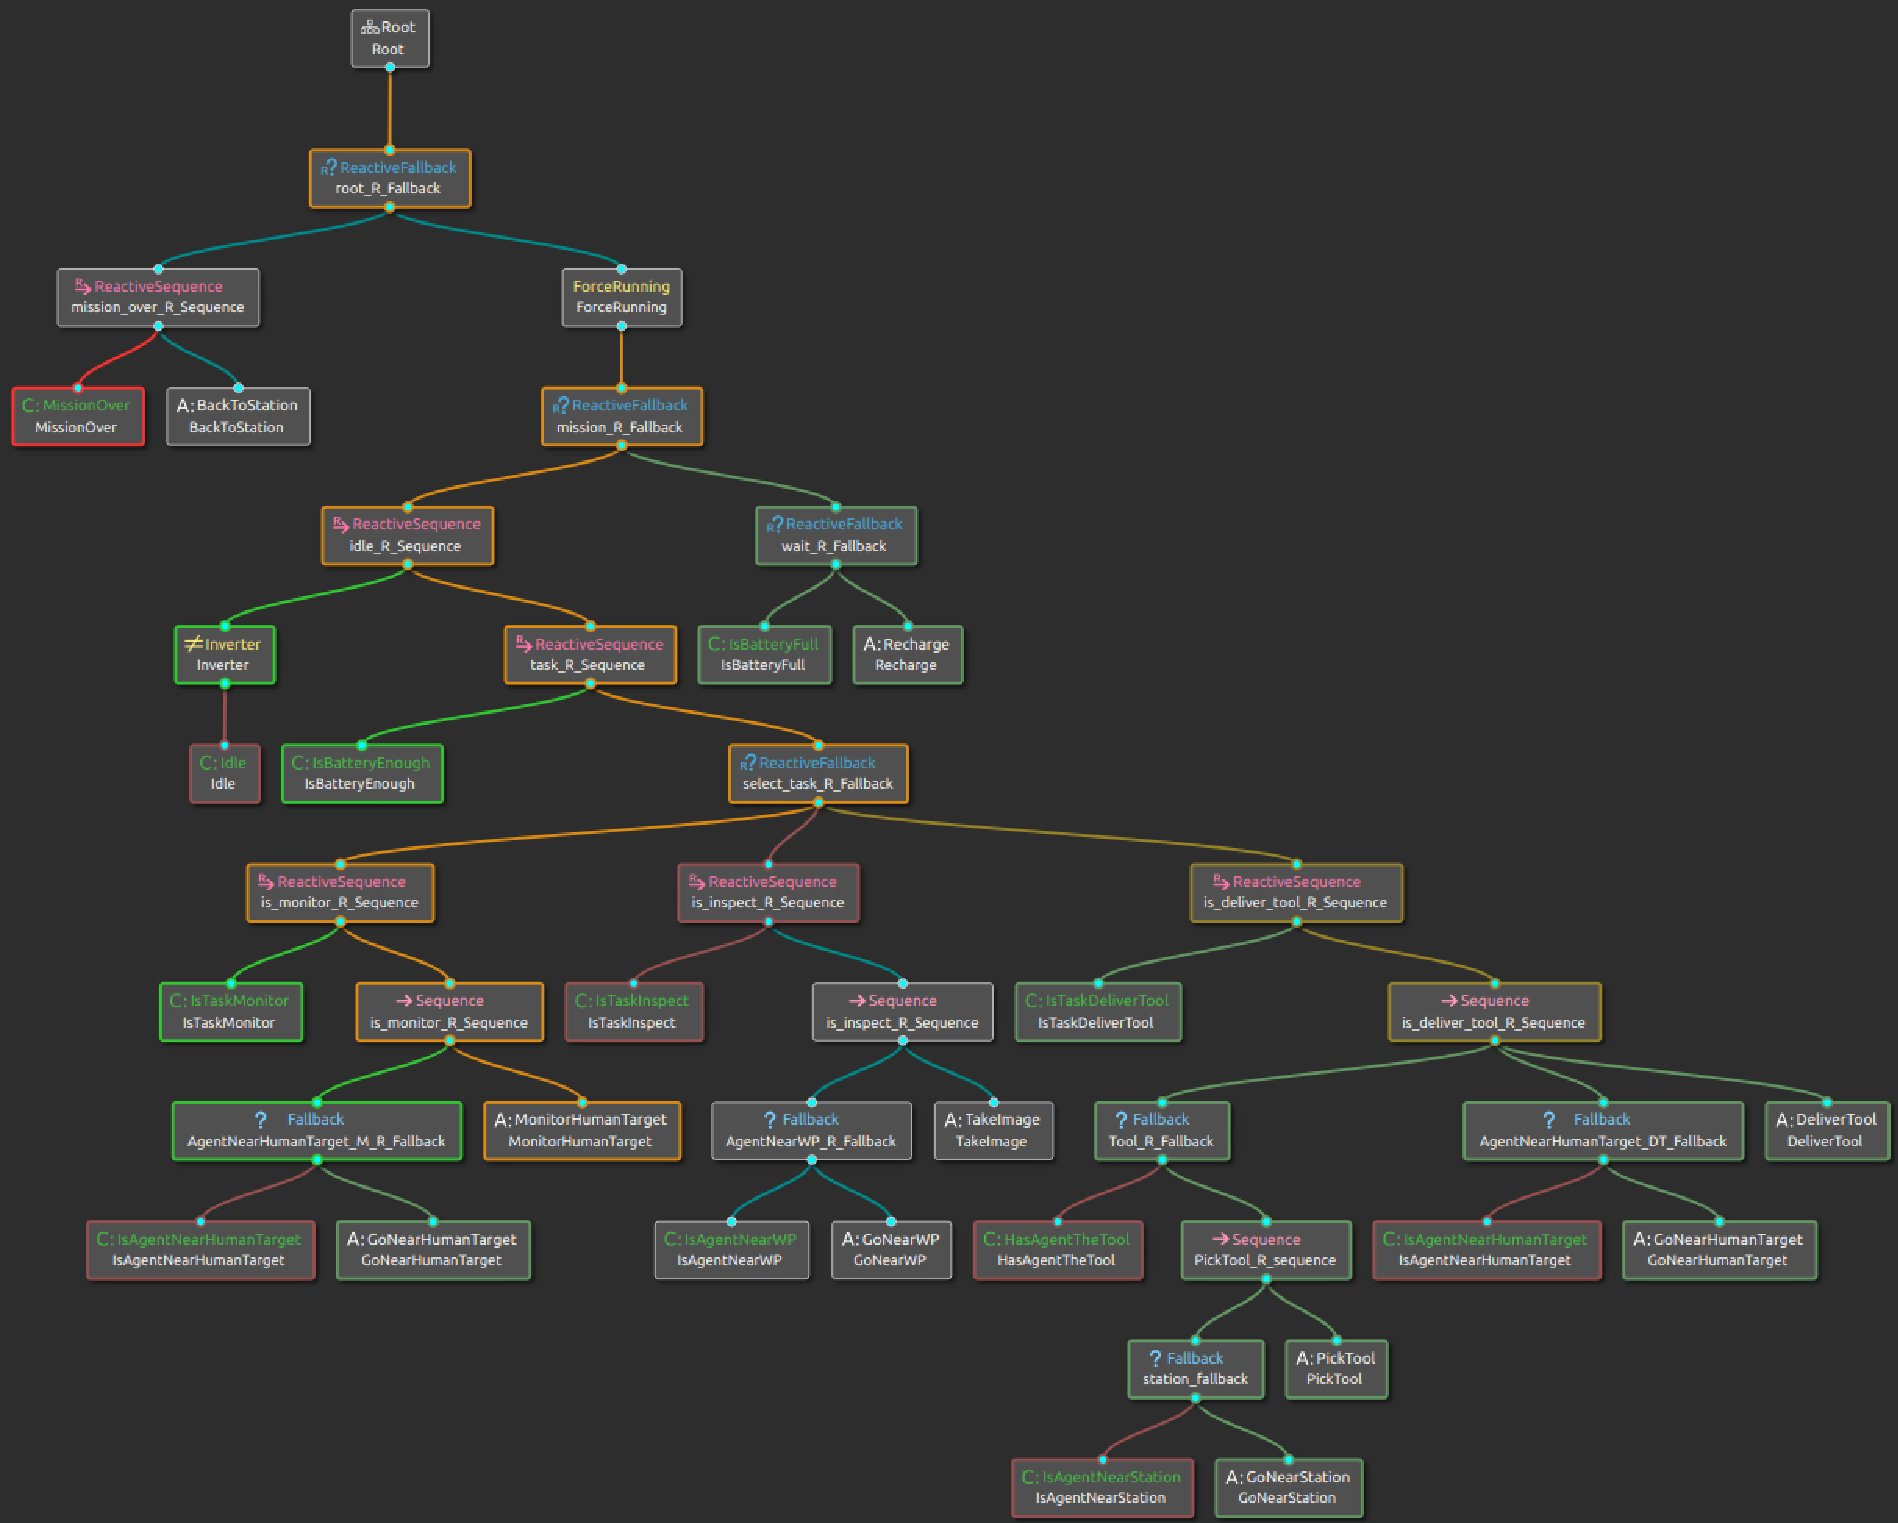
\includegraphics[width=.3\linewidth]{Results/figures/BTImprevistoMDT_1.pdf}}
    \hfill
    \subfloat[\emph{Safety Monitoring} tree is halted becouse a \emph{Tool Delivery} task took the first place in the queue]{
        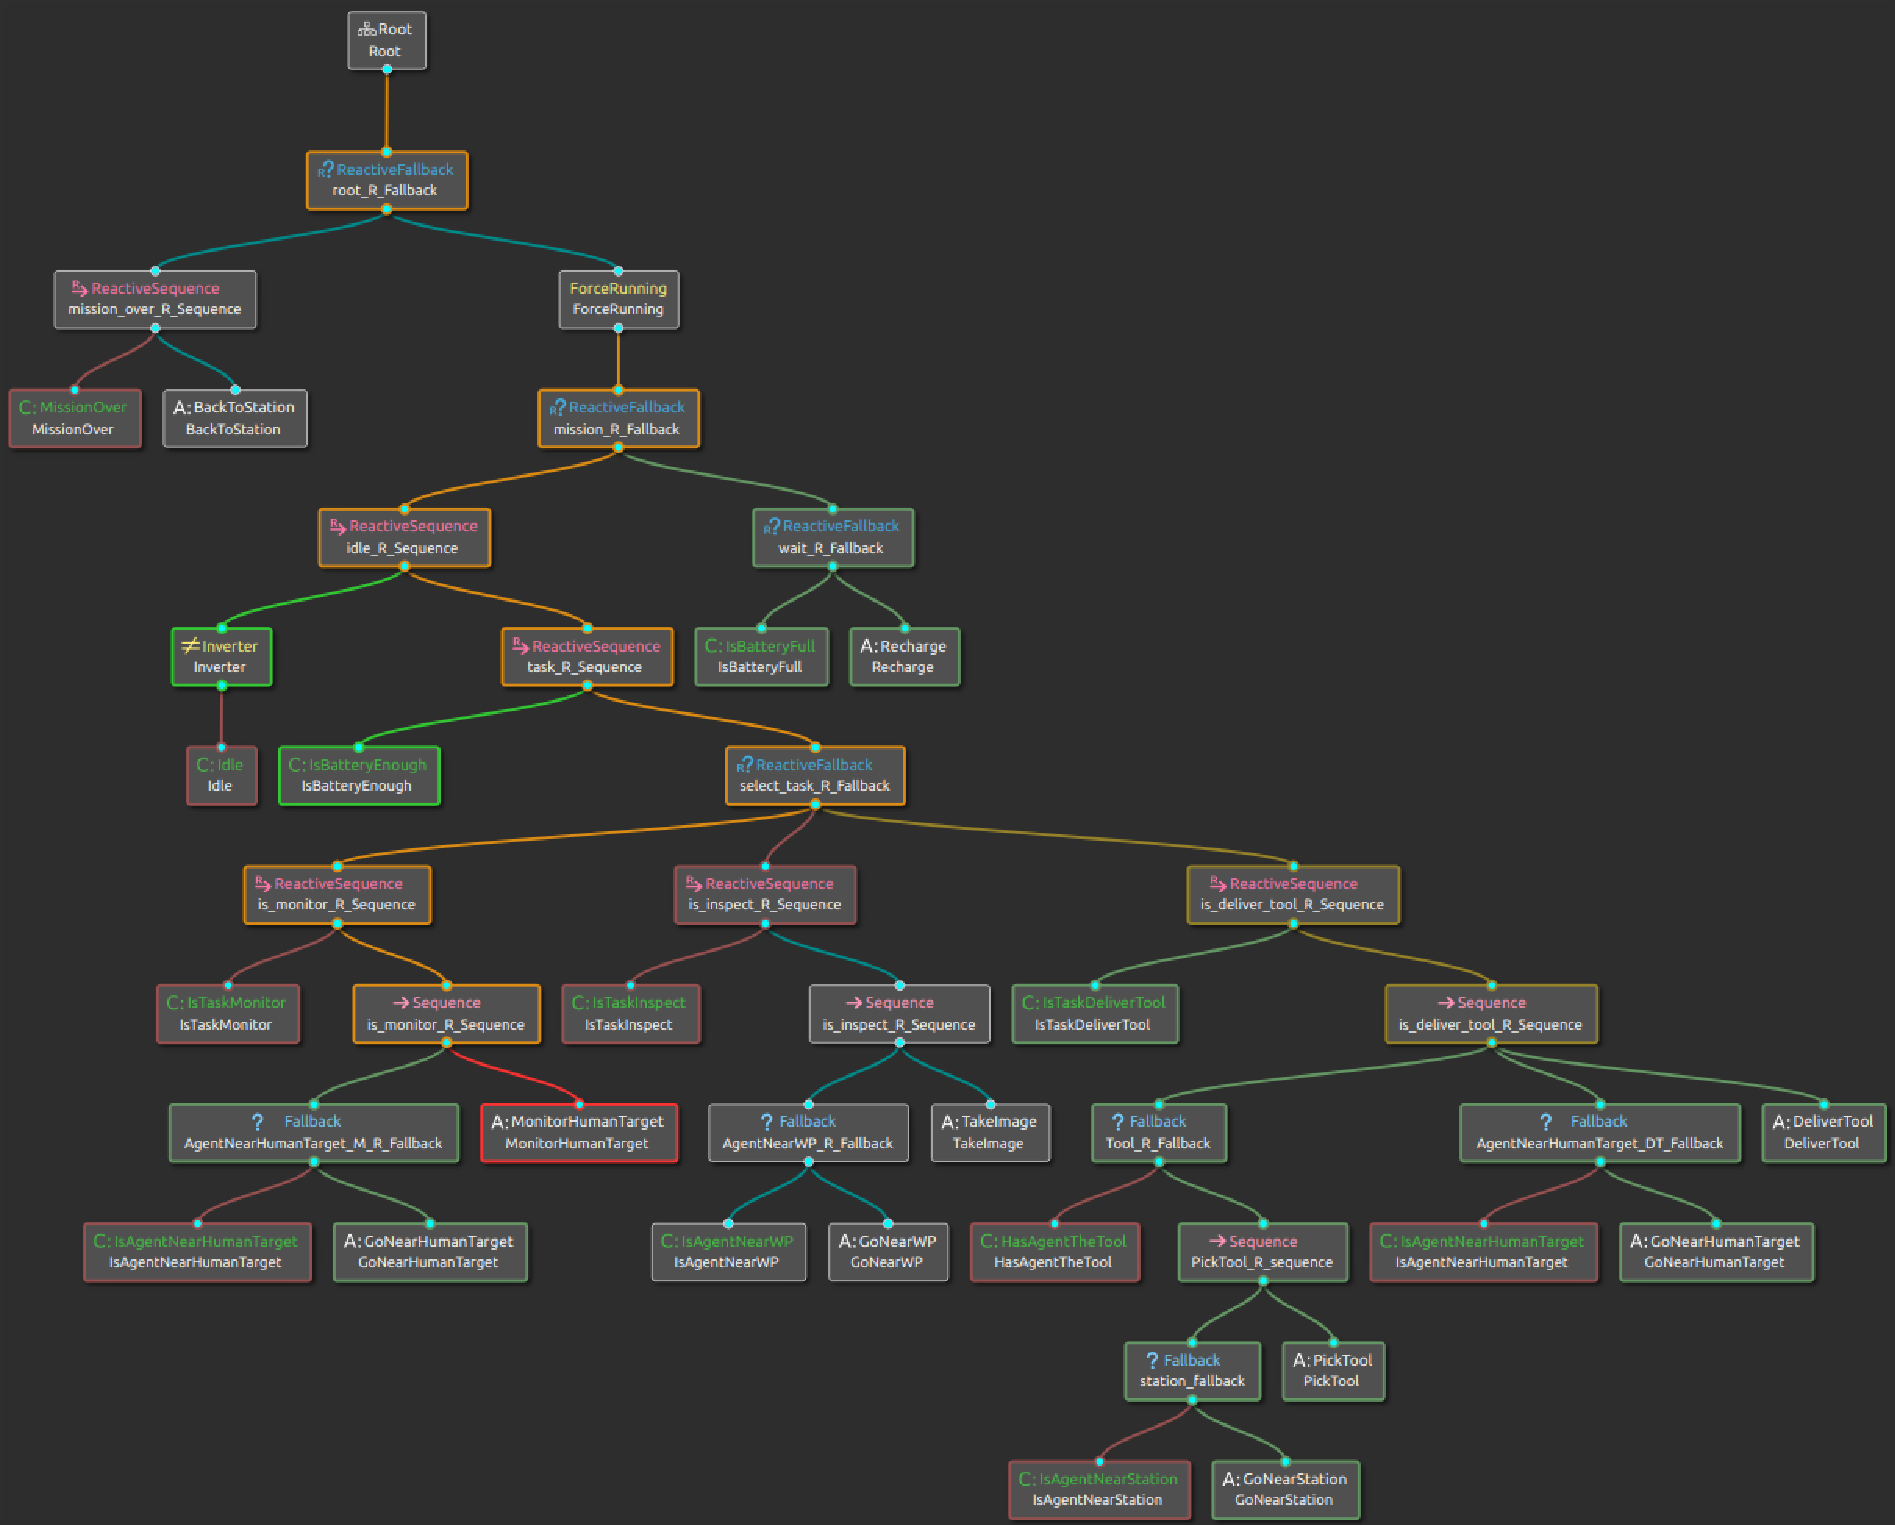
\includegraphics[width=.3\linewidth]{Results/figures/BTImprevistoMDT_2.pdf}}
    \hfill
    \subfloat[\emph{Tool Delivery} tree running]{
        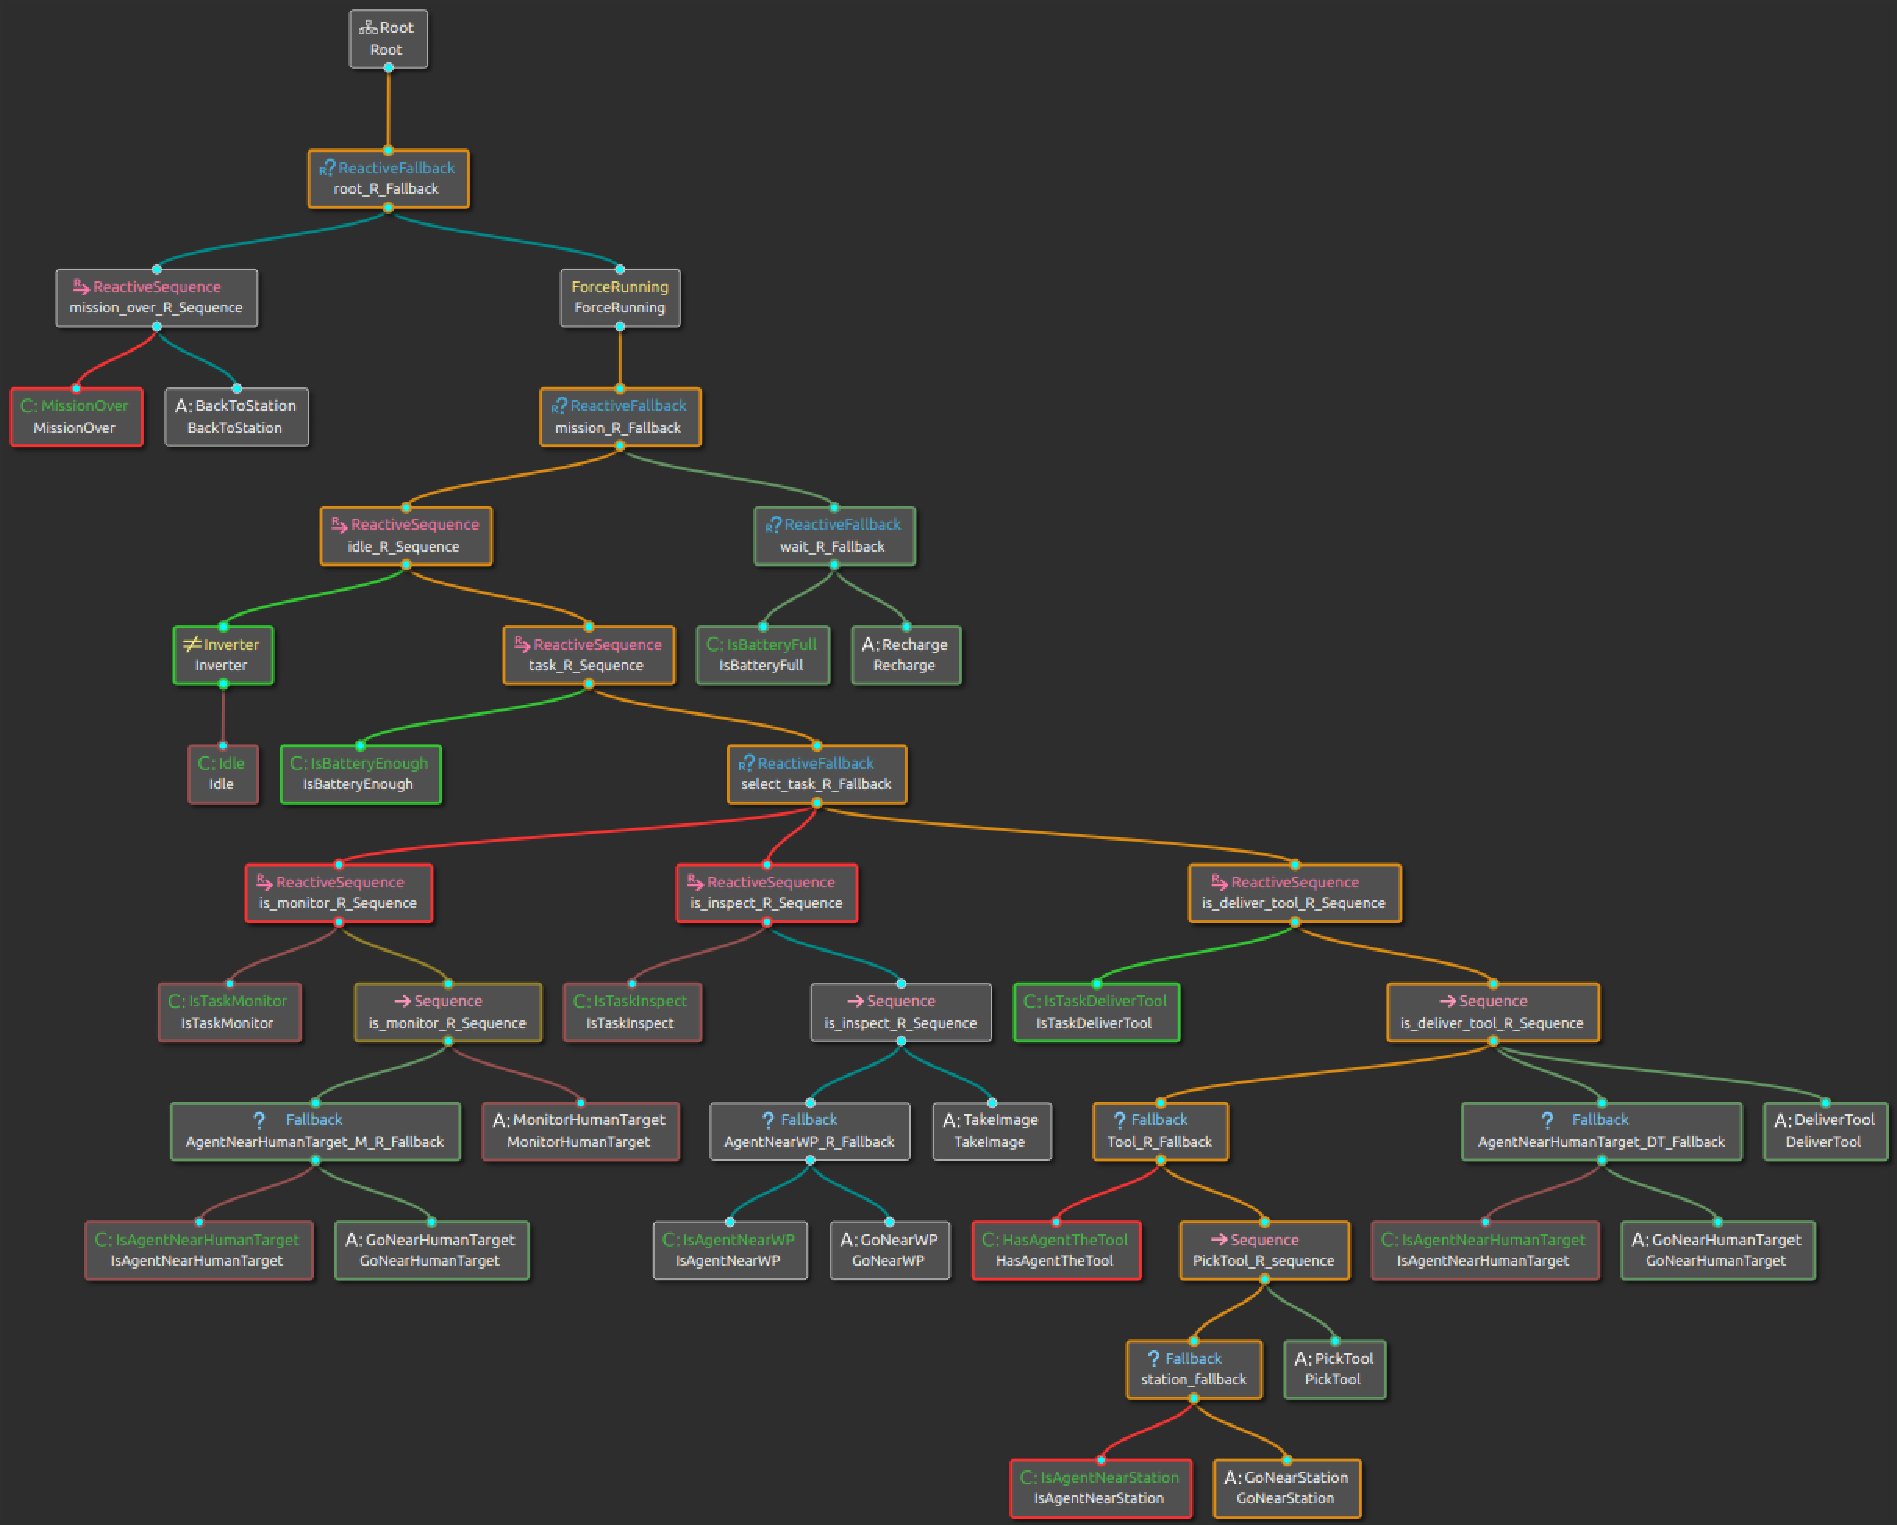
\includegraphics[width=.3\linewidth]{Results/figures/BTImprevistoMDT_3.pdf}}
    \caption{Evolution of the \gls{BT} during a change of plans. \emph{Tool Delivery} task displaces \emph{Safety Monitoring} task}
    \label{fig:event_ChangeOfPlans}
\end{figure}

After the success of the previous test, it was tested whether the \emph{High-Level Planner} is able to handle the situation when a new task with a repeated \gls{ID} arrives. For this purpose, an \emph{Inspection} task with the same \gls{ID} as the previous \emph{Tool Delivery} task was sent before the previous \emph{Tool Delivery} task was finished. The system passed the test successfully as shown in code \ref{exit:event_DuplicatedID}, the task was cancelled and deleted by the \emph{High-Level Planner} and the \gls{BT}, who halted the previous task and completed the new one successfully, remaining at the end executing the monitoring task requested at the beginning of the simulation, which has not yet finished. As the \gls{BT} simply reacted to the change of plans exactly as in the previous situation, no figure is now displayed.

\begin{lstlisting}[caption={Feedback messages printed after the arrival of a task with a repeated id. \emph{Inspection} task overwrites \emph{Tool Delivery} task}, breaklines=true, label=exit:event_DuplicatedID]
    [ WARN][/task_planner]: [incomingTask] Duplicated ID. An unfinished task is going to be deleted: task_4(DeliverTool)
    [ INFO][/task_planner]: [incomingTask] Received a New Task:
        task_4: Inspect
            Positions: (0, 0, 2) (10, 10, 2) (0, 10, 2) (10, 0, 2)
            Agent List:
    
    [ INFO][/task_planner]: [incomingTask] Allocating tasks...
    [ INFO][/task_planner]: [performTaskAllocation] Tasks Allocated:
    [ INFO][/task_planner]: [performTaskAllocation] Agent id: uav_1
        Agent type: PhysicalACW
        Task list: (2 tasks)
            task_4: Inspect
            task_3: Monitor
    
    [ INFO][/uav_1/agent]: [newTaskList] Received a NewTaskList Action
    [ INFO][/uav_1/agent]: task_4: Inspect
    [ INFO][/uav_1/agent]: [PickTool] halt requested
    [ INFO][/uav_1/agent]: [PickTool] PICK TOOL FINISHED
    [ INFO][/uav_1/agent]: [GoNearWP] Moving near WP...
    [ INFO][/uav_1/agent]: [TakeImage] Calling Lower-level controllers...
    [ INFO][/uav_1/agent]: [TakeImage] INSPECT TASK FINISHED (true)
    [ INFO][/task_planner]: [taskResultCB] (uav_1) task_4(Inspect) SUCCEEDED. Reallocating just in case...
    [ INFO][/uav_1/agent]: task_3: Monitor
    [ INFO][/uav_1/agent]: [GoNearHumanTarget] Moving near HT...
    [ INFO][/uav_1/agent]: [MonitorHumanTarget] Calling Lower-level controllers...
\end{lstlisting}

Next, the battery level was suddenly lowered to check the \gls{BT}'s reaction. The \gls{BT} immediately stopped the execution of the task to make an emergency visit to the charging station as shown in the figure \ref{fig:event_battery}. Note that the halt is not produced by \emph{Is Battery Enough?} condition node, but by the emptying of the task queue as established by the protocol. Thus, the node that stops the execution of the task should always be \emph{Idle}'s \emph{Inverter} node, not \emph{Is Battery Enough?} condition node, which is there to provide the \gls{BT} with additional robustness in case of failure. It can also be seen in the feedback showed in code \ref{exit:event_battery} that the \emph{Agent Behaviour Manager} communicated to the \emph{High-Level Planner} the detection of the unforeseen event, which triggered a replanning on its side. Note that this test was possible thanks to the functions programmed in the block in charge of faking the \gls{UAV}'s battery.

\begin{figure}[htbp]
    \centering
    \subfloat[\emph{Safety Monitoring} tree running]{
        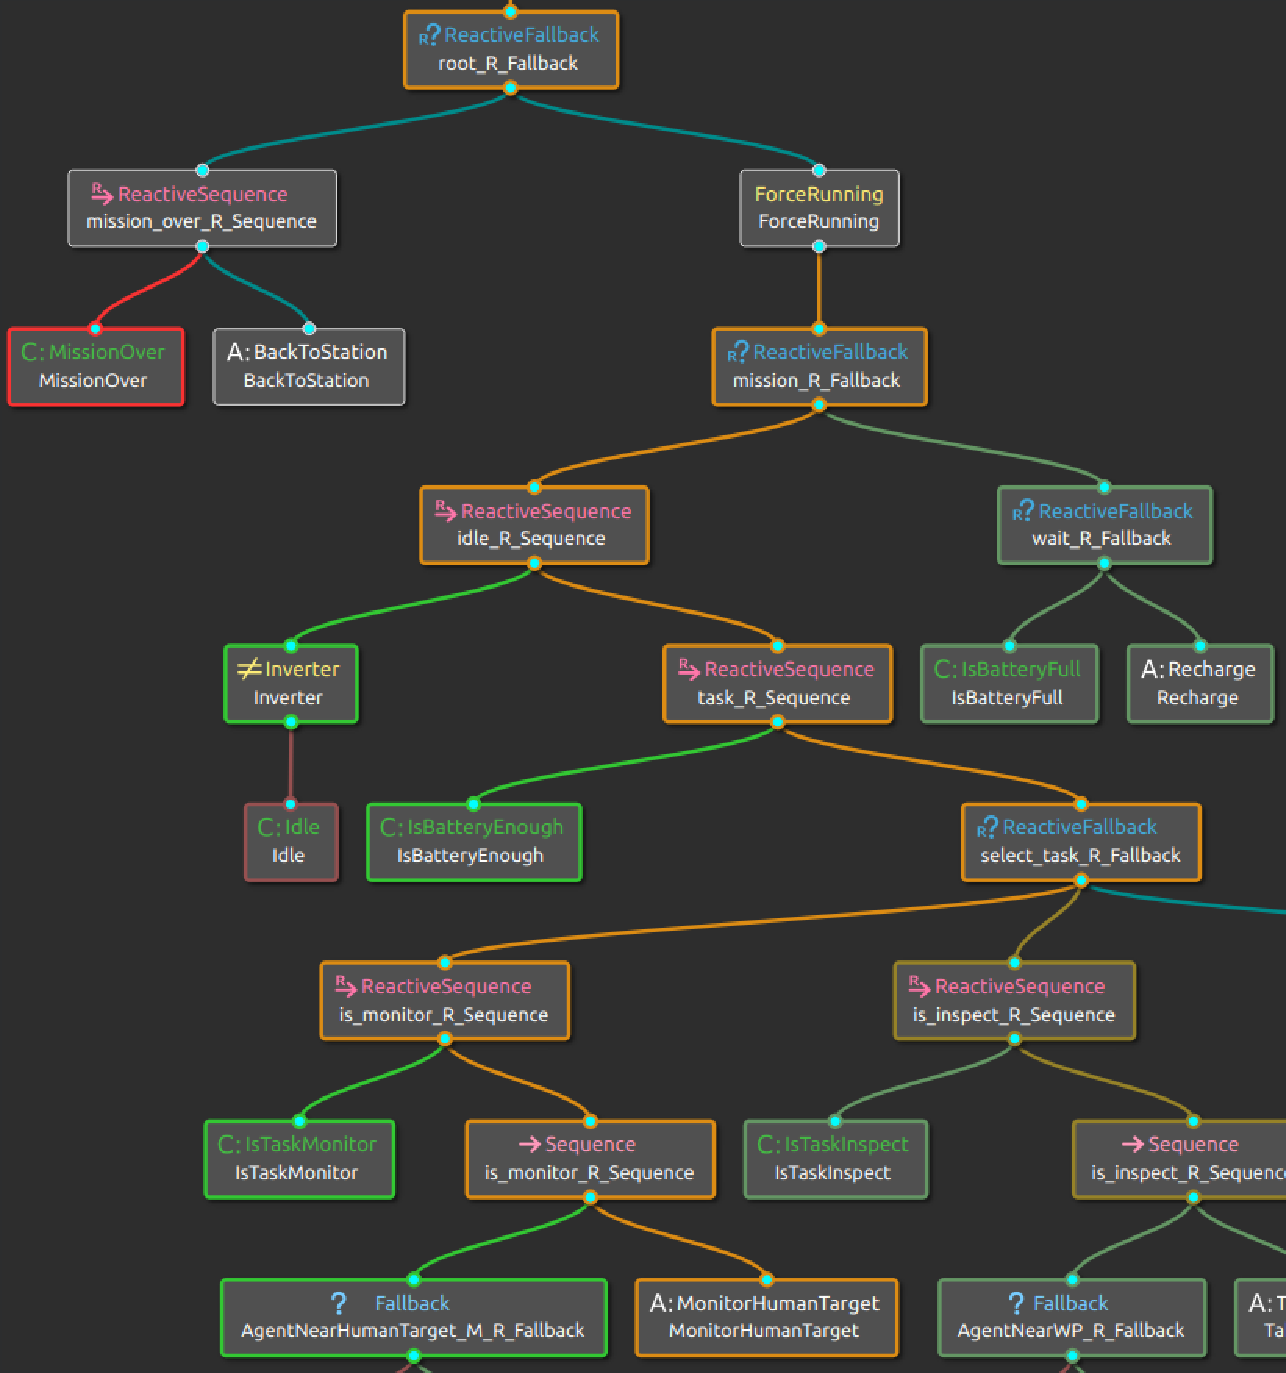
\includegraphics[width=.3\linewidth]{Results/figures/BTImprevistoBat_1.pdf}}
    \hfill
    \subfloat[\emph{Safety Monitoring} tree is halted becouse \emph{Idle}'s \emph{Inverter} node returns \emph{FAILURE}]{
        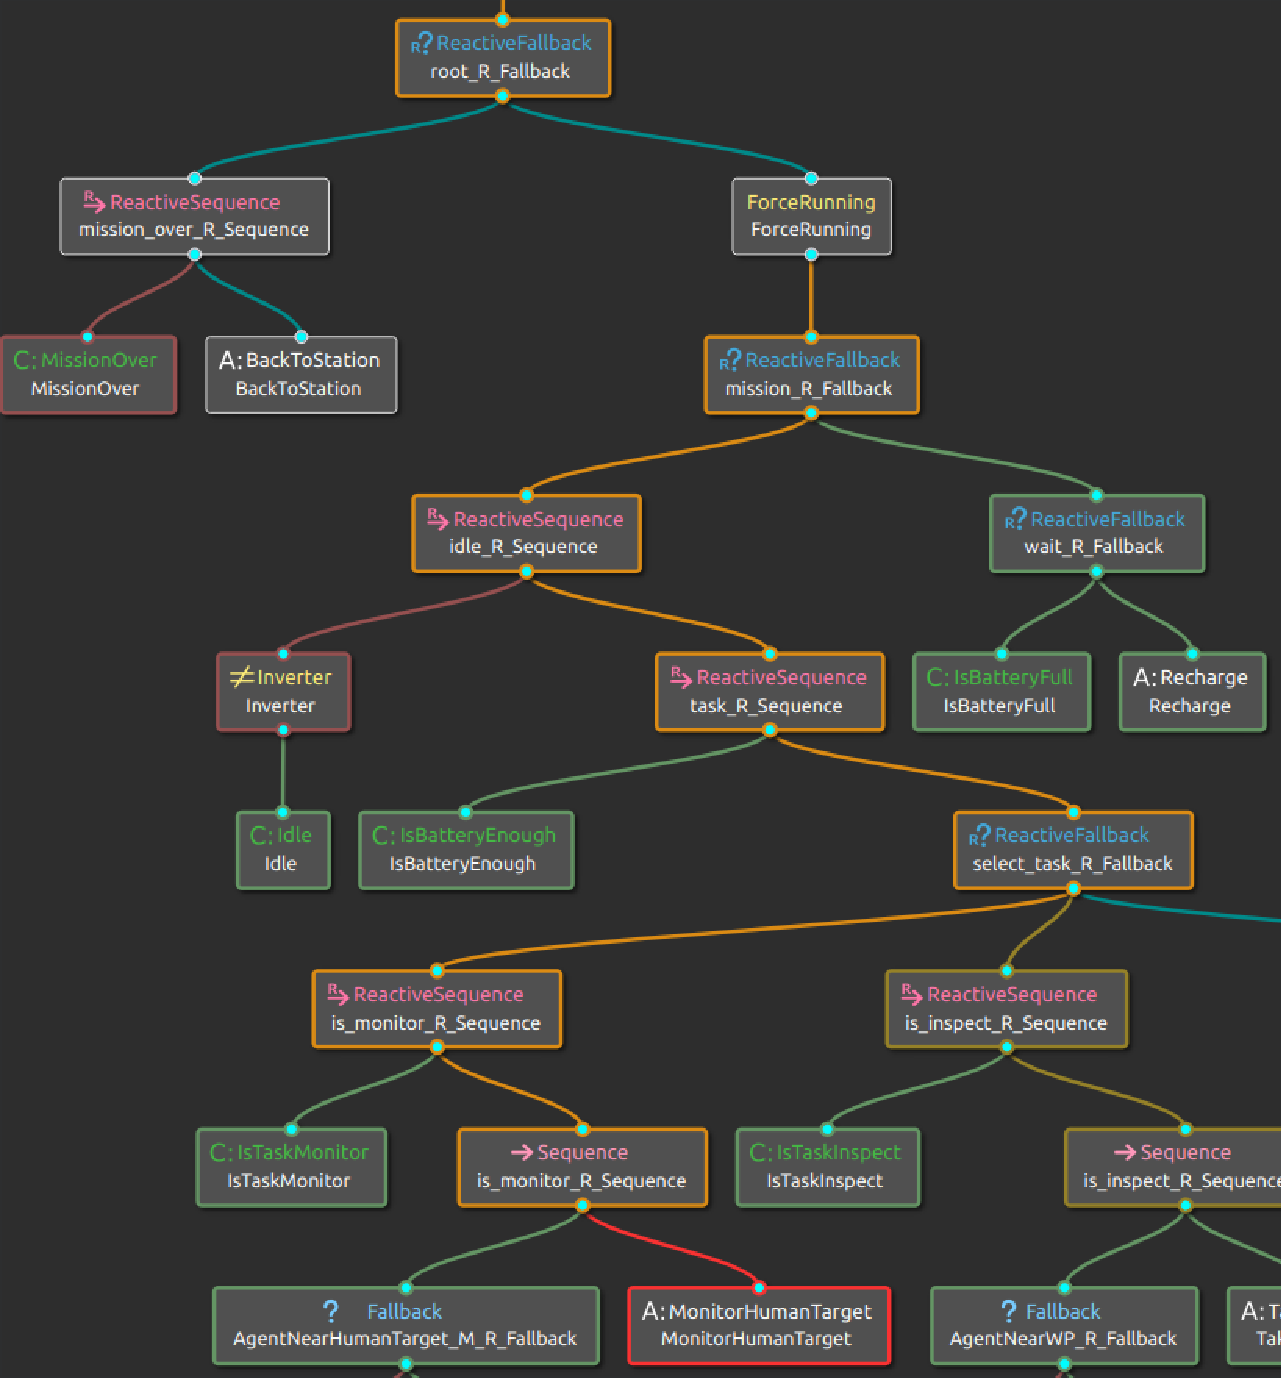
\includegraphics[width=.3\linewidth]{Results/figures/BTImprevistoBat_2.pdf}}
    \hfill
    \subfloat[\emph{Recharge} node running]{
        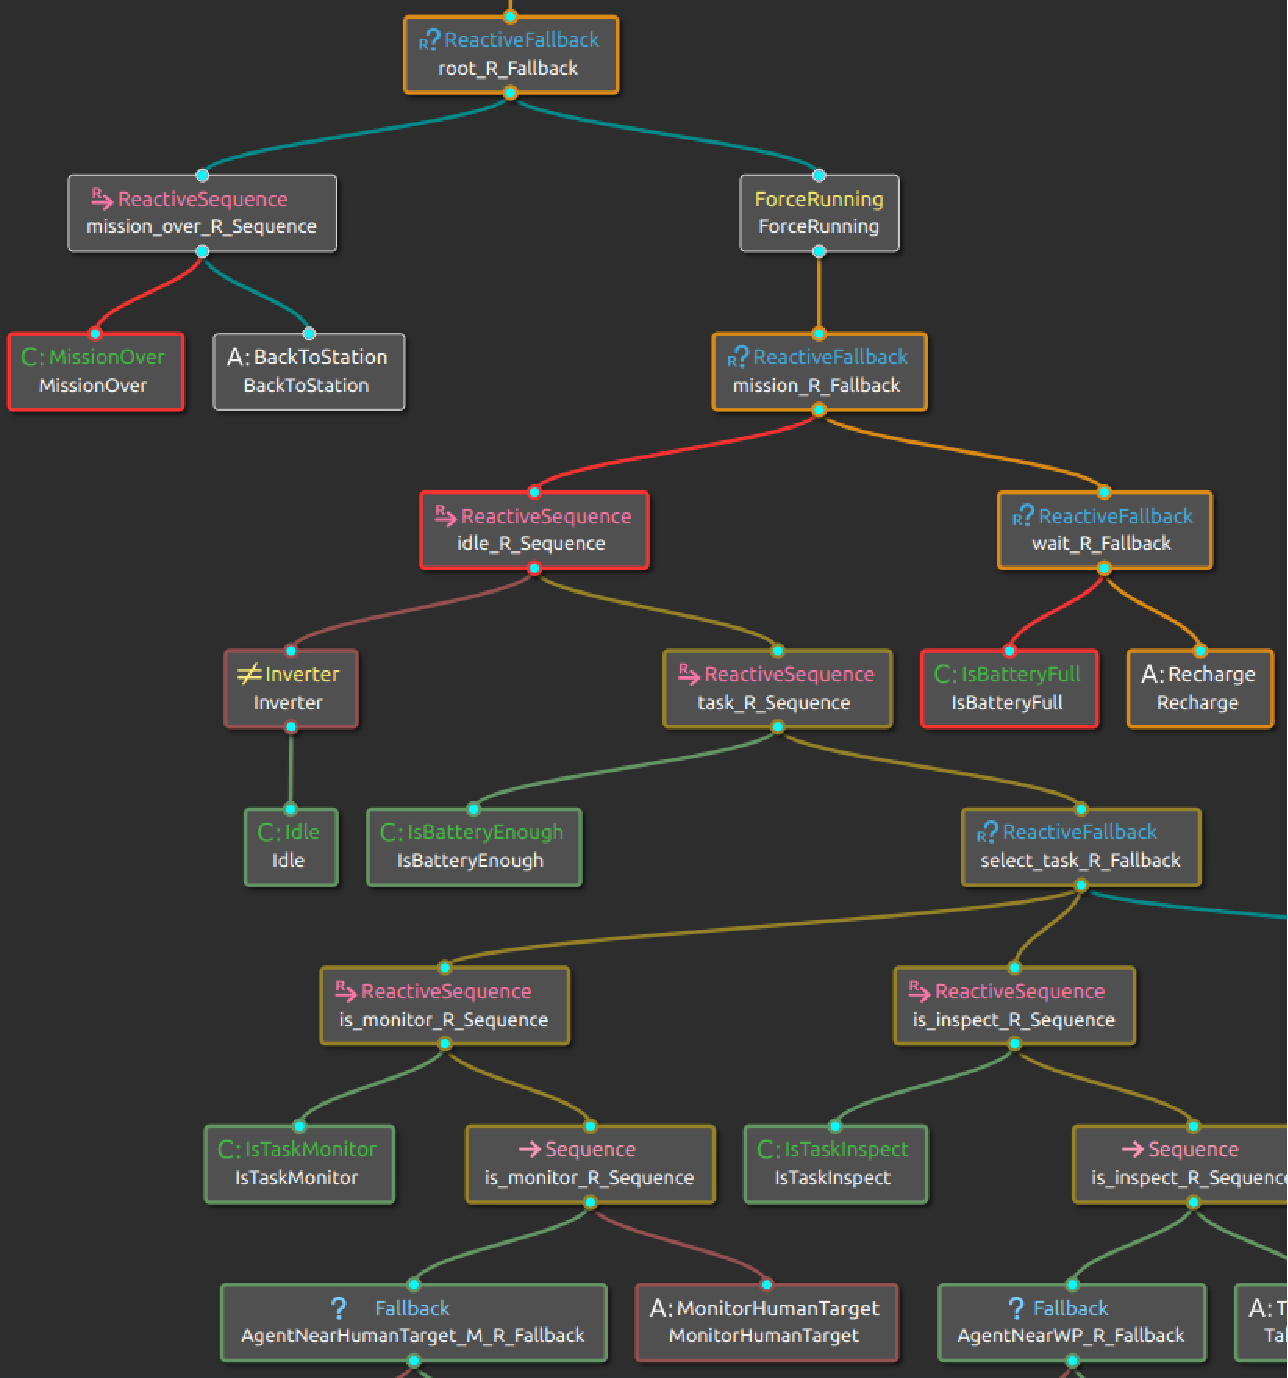
\includegraphics[width=.3\linewidth]{Results/figures/BTImprevistoBat_3.pdf}}
    \caption{Emergency protocol in the event of an insufficient battery}
    \label{fig:event_battery}
\end{figure}

\begin{lstlisting}[caption={Feedback messages printed after insufficient battery event}, breaklines=true, label=exit:event_battery]
    [ WARN][/uav_1/agent]: [isBatteryEnough] Advertising that battery_enough_ = false
    [ INFO][/uav_1/agent]: [MonitorHumanTarget] halt requested
    [ INFO][/uav_1/agent]: [MonitorHumanTarget] MONITOR TASK FINISHED (false)
    [ INFO][/uav_1/agent]: [Recharge] Calling take_off
    [ INFO][/uav_1/agent]: [Recharge] Moving to recharging station
    [ INFO][/uav_1/agent]: [Recharge] Calling land
    [ INFO][/uav_1/agent]: [Recharge] Charging...
    
    [ WARN][/task_planner]: [batteryEnoughCB] (uav_1) Noticed that battery_enough_ = false
    [ INFO][/task_planner]: [performTaskAllocation] Tasks Allocated:
    [ INFO][/task_planner]: [performTaskAllocation] Agent id: uav_1
        Agent type: PhysicalACW
        Task list: (0 tasks)
    
    [ INFO][/uav_1/agent]: [newTaskList] Received a NewTaskList Action
\end{lstlisting}

At this point it is important to mention that a \emph{Recharge} task has not been implemented and therefore recharges cannot be planned as such, instead in the current solution the \emph{High-Level Planner} makes the \gls{ACW} recharge by not having any task queued. To make it stop recharging the planner only has to assign a task to it, either when the battery is full or before. Using the battery faker again, the battery was set to maximum and it was found that a new replanning took place and the \gls{BT} started the \gls{ACW} again (see code \ref{exit:event_batteryOK}). The evolution of the \gls{BT} is the same as shown in figures \ref{fig:BTinitialization} and \ref{fig:NoIdle_DeliverToolTaskTree} but with the difference that now the task is of the \emph{Safety Monitoring} type.

\begin{lstlisting}[caption={Feedback messages printed after enough battery event}, breaklines=true, label=exit:event_batteryOK]
    [ WARN][/uav_1/agent]: [isBatteryEnough] Advertising that battery_enough_ = true

    [ WARN][/task_planner]: [batteryEnoughCB] (uav_1) Noticed that battery_enough_ = true
    [ INFO][/task_planner]: [performTaskAllocation] Tasks Allocated:
    [ INFO][/task_planner]: [performTaskAllocation] Agent id: uav_1
        Agent type: PhysicalACW
        Task list: (1 tasks)
            task_3: Monitor
    
    [ INFO][/uav_1/agent]: [newTaskList] Received a NewTaskList Action
    [ INFO][/uav_1/agent]: task_3: Monitor
    [ INFO][/uav_1/agent]: [Recharge] halt requested
    [ INFO][/uav_1/agent]: [GoNearHumanTarget] Moving near HT...
    [ INFO][/uav_1/agent]: [MonitorHumanTarget] Calling Lower-level controllers...
\end{lstlisting}

The other possible emergency situation is the loss of connection between the two blocks that make up this work. To test this case the process that was running the \emph{High-Level Planner} was killed. The emergency situation was successfully detected by the \gls{BT} after the maximum timeout time had elapsed, after which the emergency protocol was activated and the \gls{ACW} was directed to the charging station. As the emergency protocol is the same, the evolution of the \gls{BT} in this scenario is the same as shown in figure \ref{fig:event_battery}. Code \ref{exit:event_AgentConnection} displays the feedback messages that are printed by the \emph{Agent Behavior Manager} block.

\begin{lstlisting}[caption={Feedback messages printed by the \emph{Agent Behavior Manager} block after a connection loss}, breaklines=true, label=exit:event_AgentConnection]
    [ WARN][/task_planner]: Shutdown request received.
    [ WARN][/task_planner]: Reason given for shutdown: [user request]
    
    [ WARN][/uav_1/agent]: [checkBeaconTimeout] Beacon timeout. Disconnection detected. Emptying the task queue.
    [ INFO][/uav_1/agent]: [MonitorHumanTarget] halt requested
    [ INFO][/uav_1/agent]: [MonitorHumanTarget] MONITOR TASK FINISHED (false)
    [ INFO][/uav_1/agent]: [Recharge] Calling take_off
    [ INFO][/uav_1/agent]: [Recharge] Moving to recharging station
    [ INFO][/uav_1/agent]: [Recharge] Calling land
    [ INFO][/uav_1/agent]: [Recharge] Charging...
\end{lstlisting}

Finally, in a new simulation, during a \emph{Safety Monitoring} task, the \emph{Mission Over} signal was sent to observe the completion of both blocks. The \emph{Agent Behaviour Manager} directed the \gls{ACW} to the base station and then the \gls{BT} and the entire block were terminated (see Fig. \ref{fig:event_MissionOver}). The \emph{High-Level Planner}, after detecting the signal, waited for all \glspl{ACW} to finish and then shut down as well (see code \ref{exit:event_MissionOver}).

% \ref{fig:event_MissionOver} Groot y terminal del proceso de mission over
\begin{figure}[htbp]
    \centering
    \subfloat[\emph{Safety Monitoring} tree running]{
        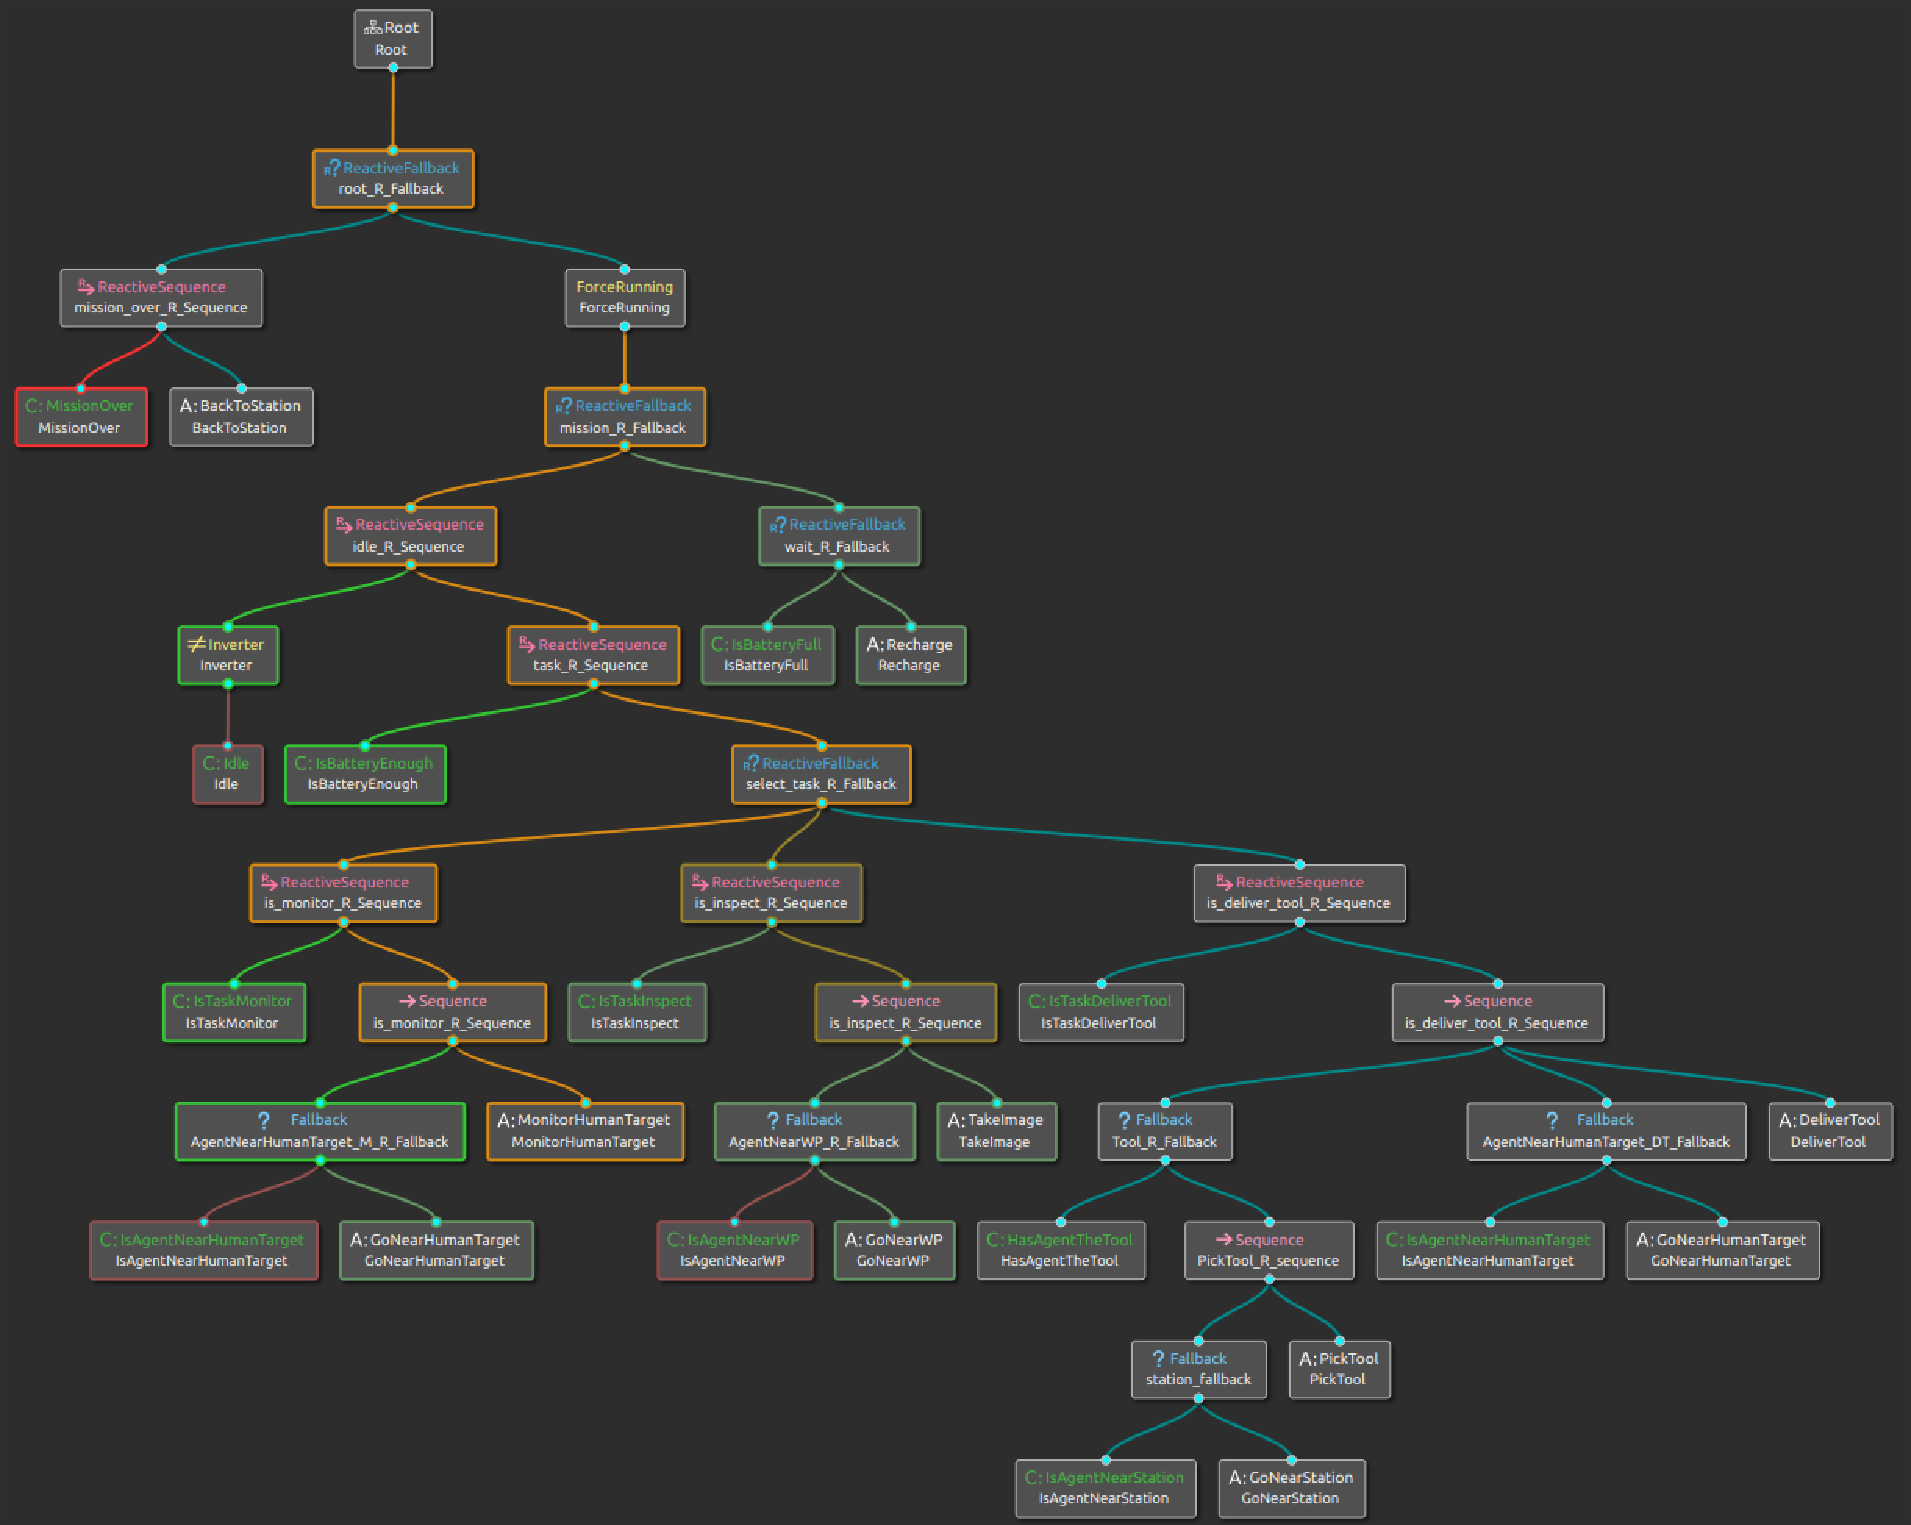
\includegraphics[width=.45\linewidth]{Results/figures/BTMO_1.pdf}}
    \hfill
    \subfloat[\emph{Safety Monitoring} tree is halted becouse \emph{Mission Over?} condition is true. \emph{Back to Station} node running]{
        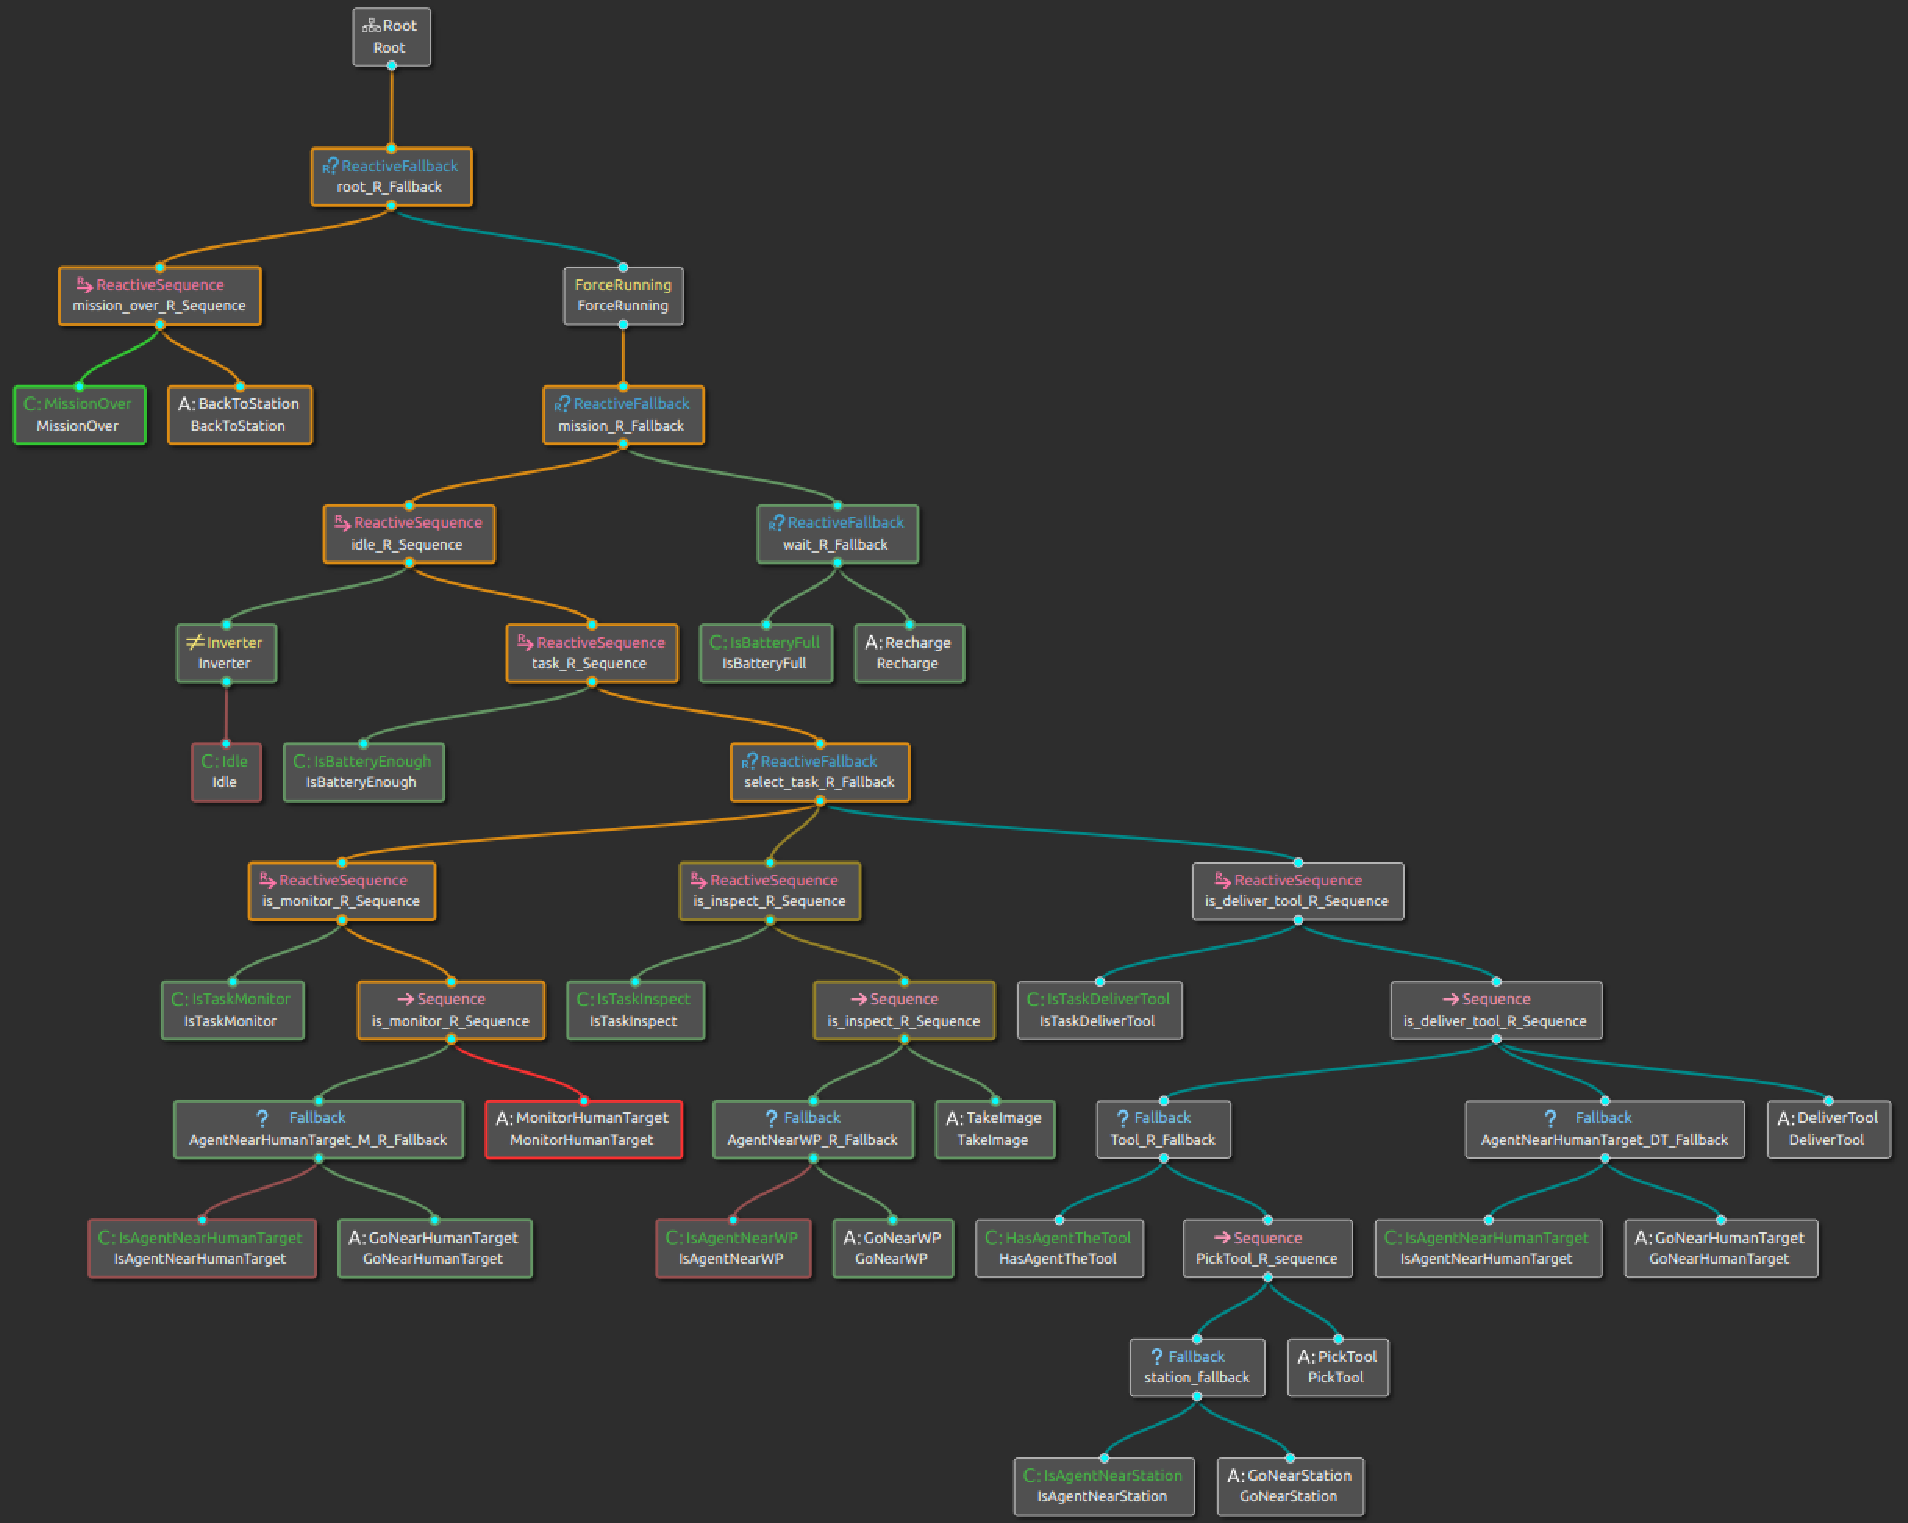
\includegraphics[width=.45\linewidth]{Results/figures/BTMO_2.pdf}}
    \\
    \subfloat[\emph{Back to Station} node returns \emph{SUCCESS} so \gls{BT}'s root does the same]{
        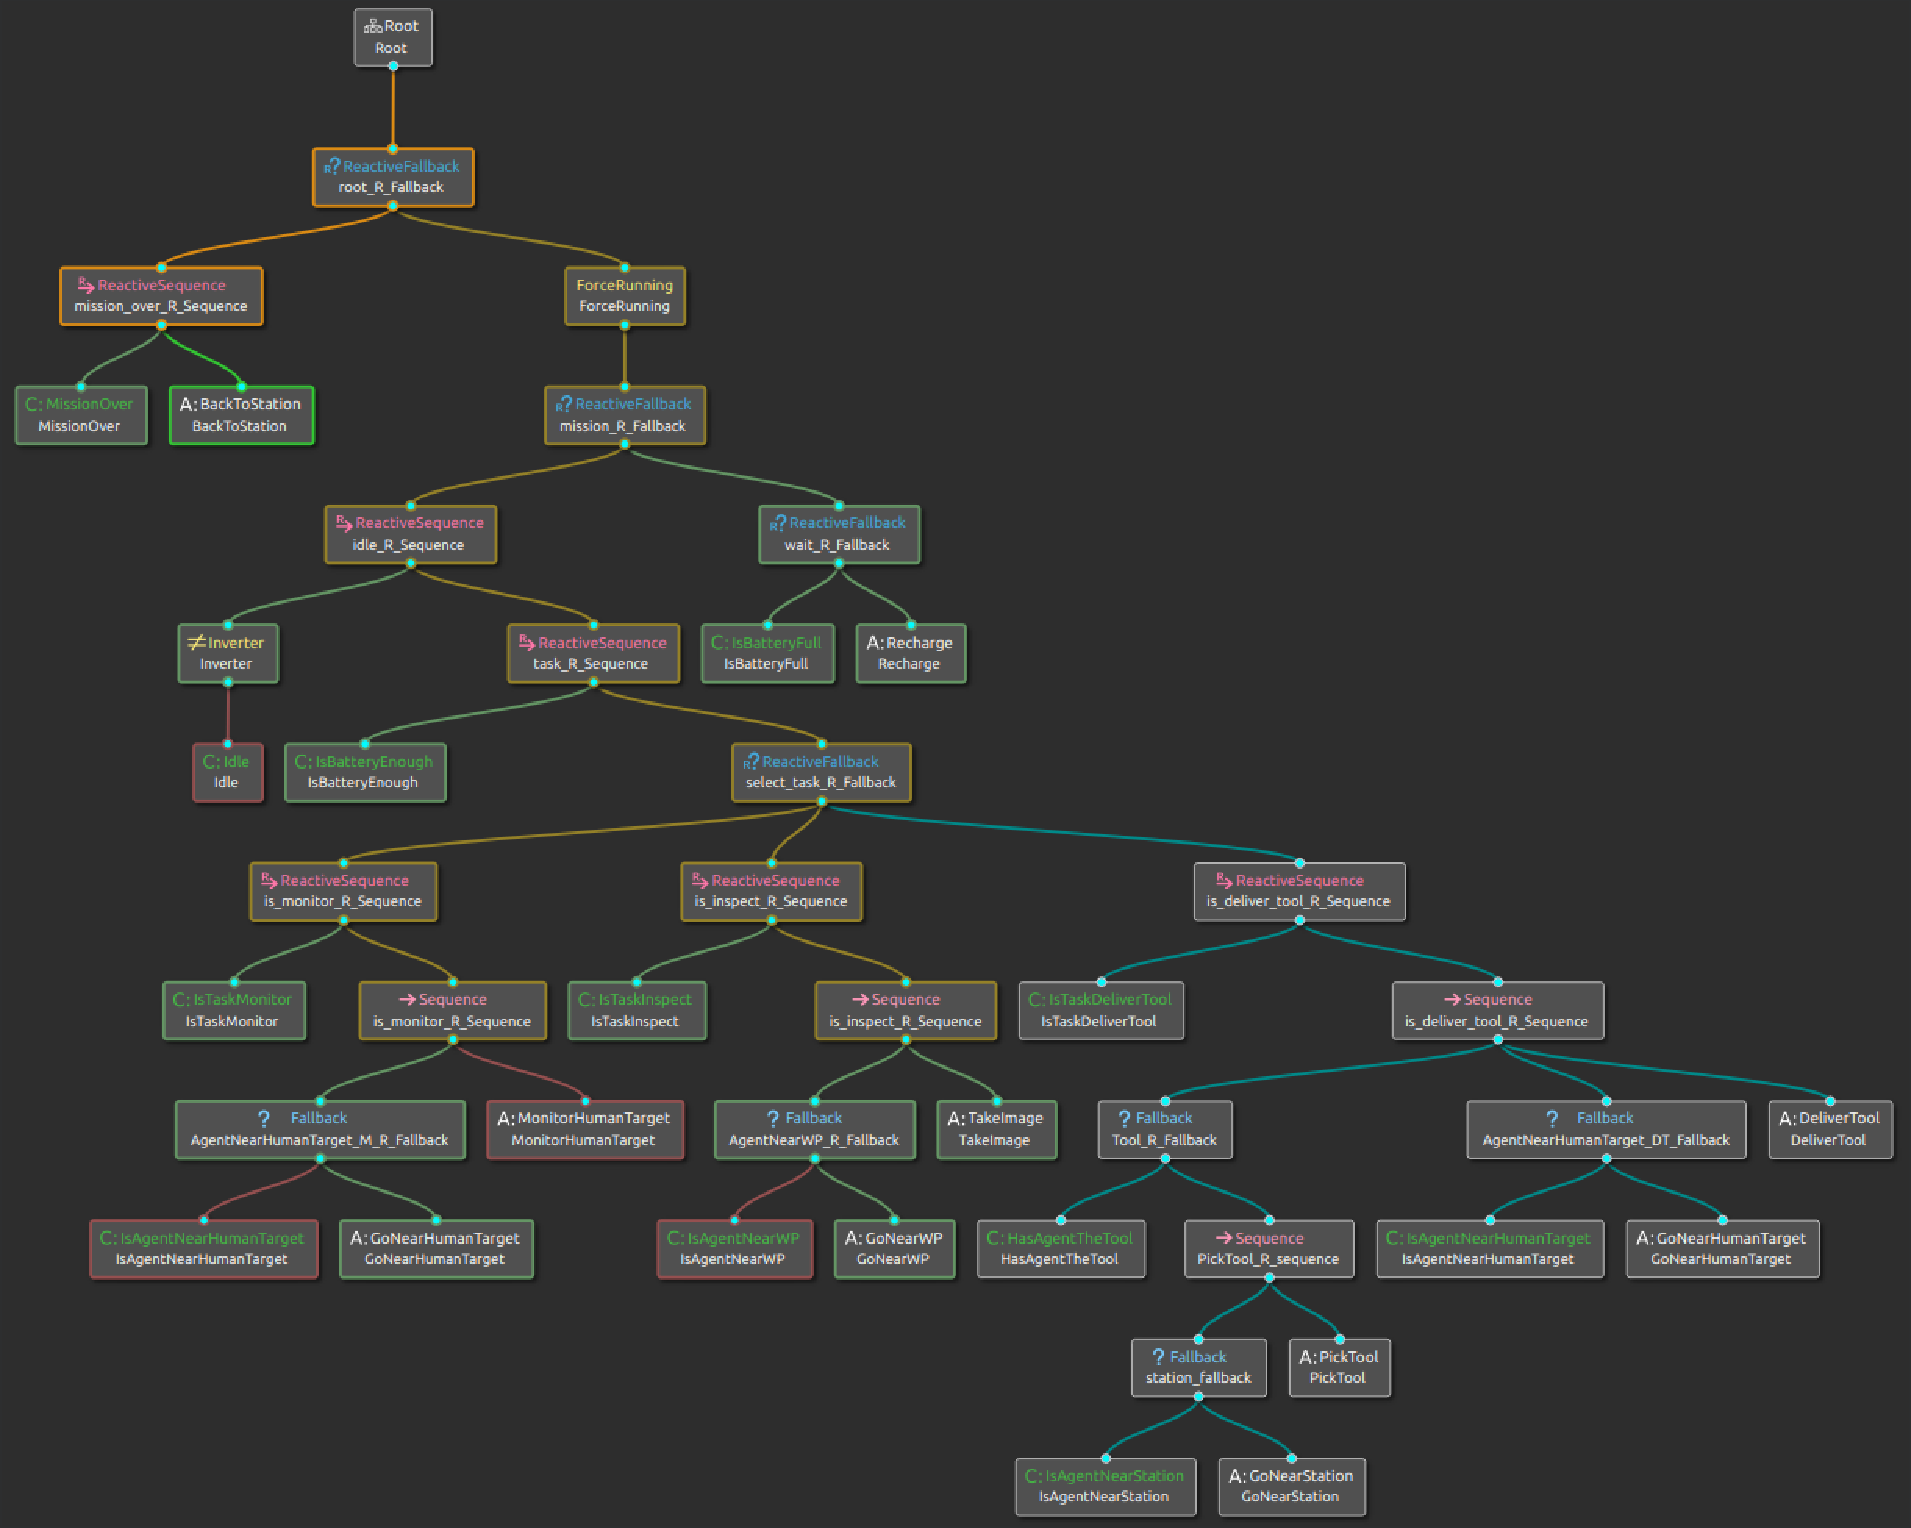
\includegraphics[width=.45\linewidth]{Results/figures/BTMO_3.pdf}}
        \hfill
    \subfloat[\emph{Agent Behaviour Manager} block exits the main while and \gls{BT} is powered off]{
        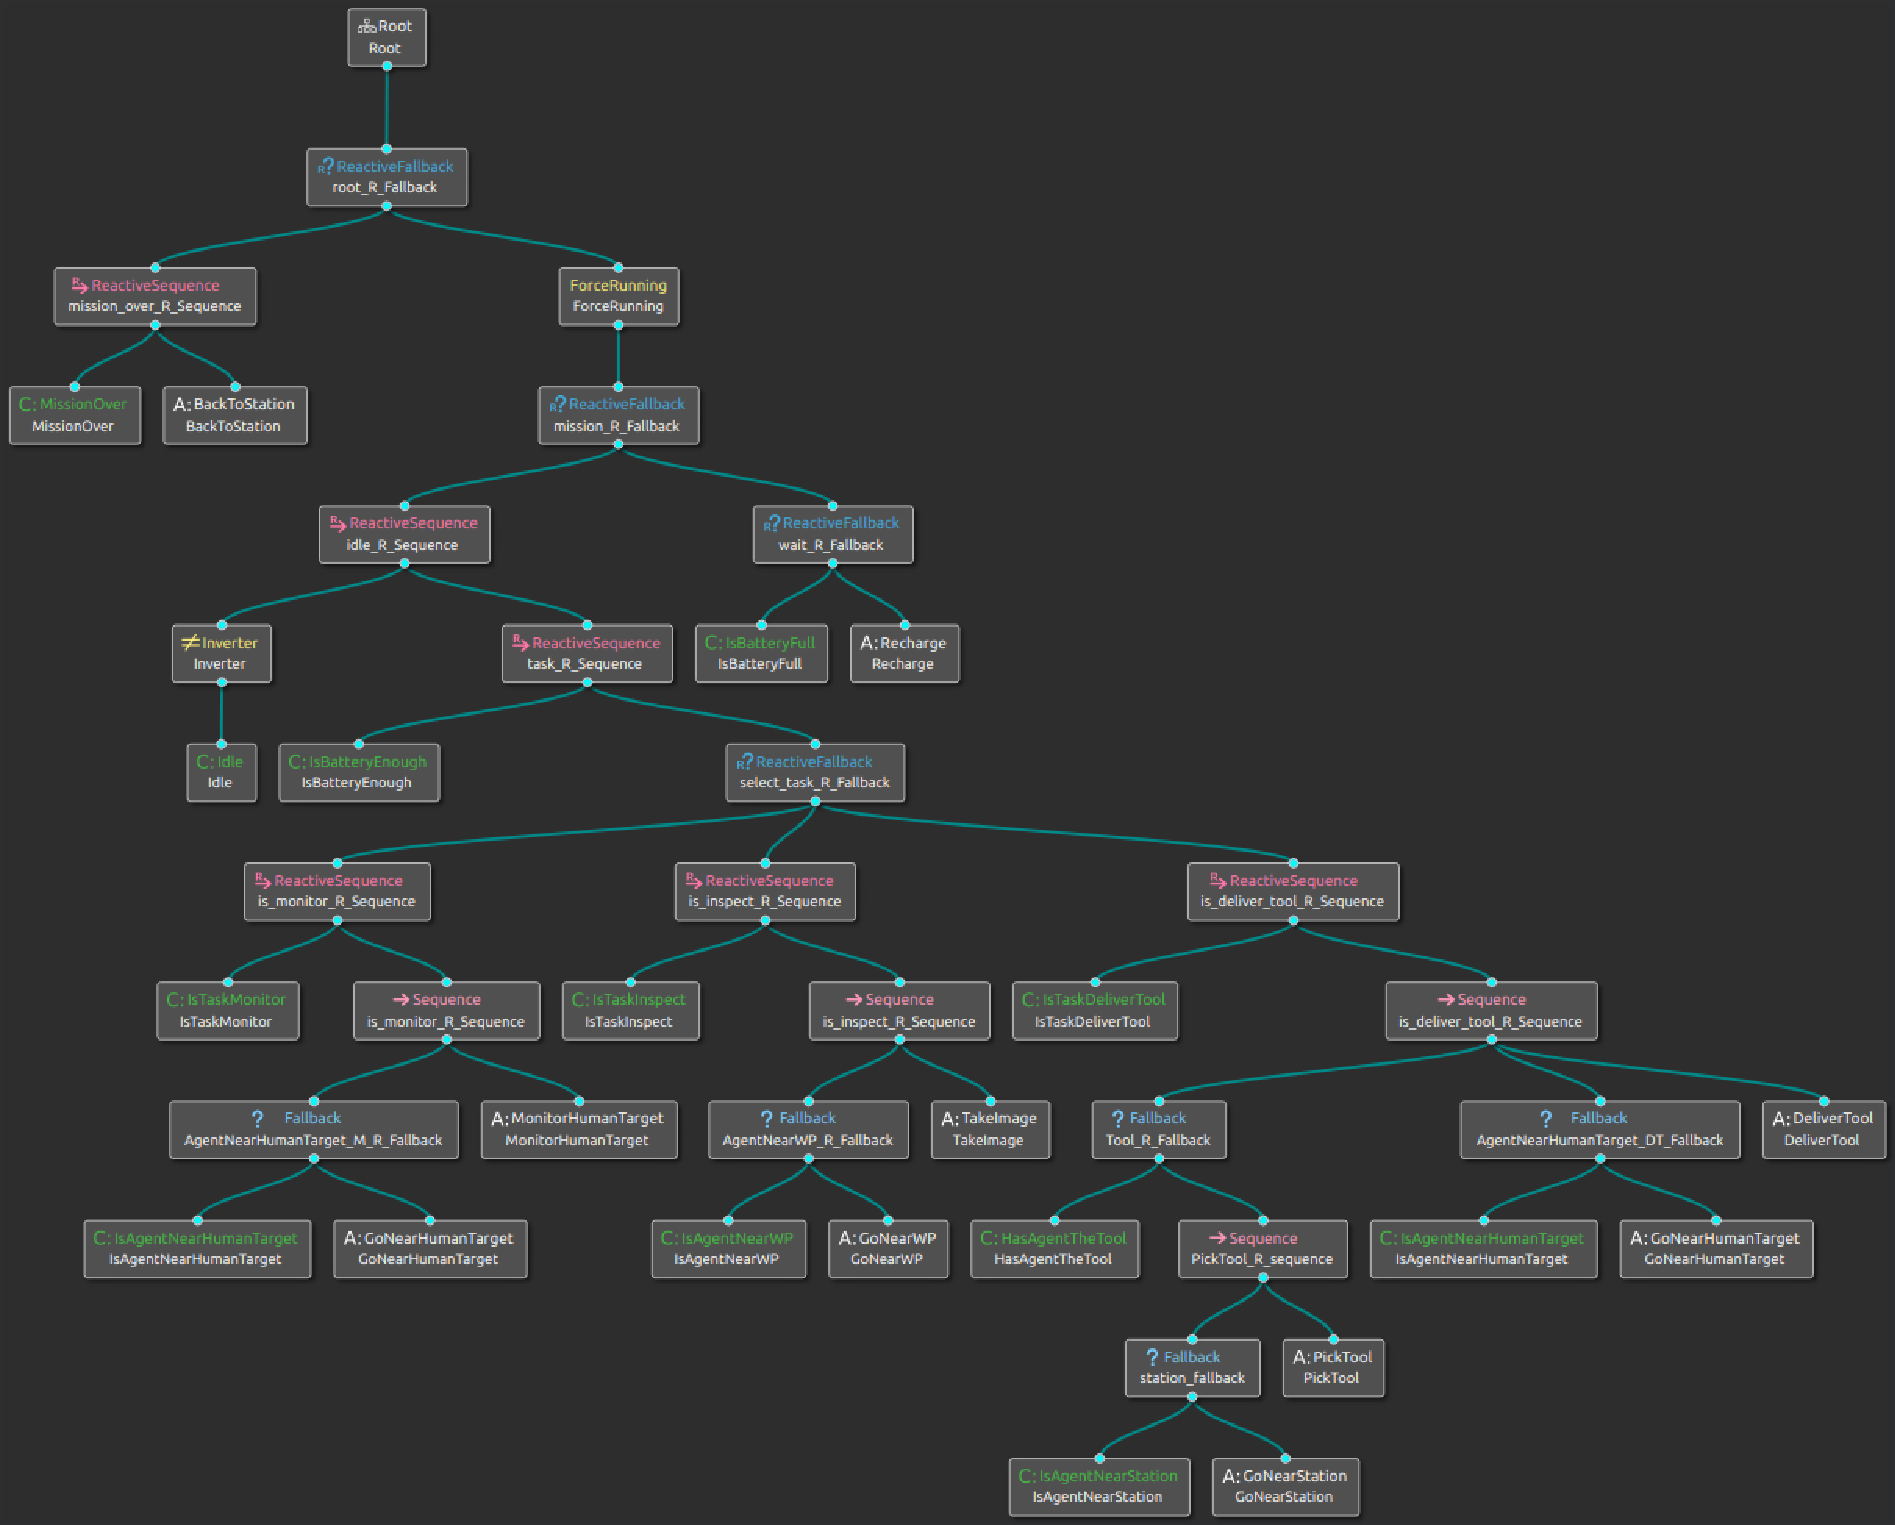
\includegraphics[width=.45\linewidth]{Results/figures/BTMO_4.pdf}}
    \caption{\gls{BT} leading \gls{ACW} to station and shutting down after the arrival of a mission over signal}
    \label{fig:event_MissionOver}
\end{figure}

\begin{lstlisting}[caption={Feedback messages printed after mission over signal}, breaklines=true, label=exit:event_MissionOver]
    [ INFO][/task_planner]: [Planner] Mission Over. Waiting for the agents to finish

    [ INFO][/uav_1/agent]: [MonitorHumanTarget] halt requested
    [ INFO][/uav_1/agent]: [MonitorHumanTarget] MONITOR TASK FINISHED (false)
    [ INFO][/uav_1/agent]: [BackToStation] Emptying the Queue...
    [ INFO][/uav_1/agent]: [BackToStation] Calling take_off
    [ INFO][/uav_1/agent]: [BackToStation] Moving to station
    [ INFO][/uav_1/agent]: [BackToStation] Calling land

    [ INFO][/uav_1/agent]: [BackToStation] halt requested
    [ INFO][/uav_1/agent]: [GoNearHumanTarget] halt requested
    [ INFO][/uav_1/agent]: [MonitorHumanTarget] halt requested
    [ INFO][/uav_1/agent]: [GoNearWP] halt requested
    [ INFO][/uav_1/agent]: [TakeImage] halt requested
    [ INFO][/uav_1/agent]: [GoNearStation] halt requested
    [ INFO][/uav_1/agent]: [PickTool] halt requested
    [ INFO][/uav_1/agent]: [GoNearHumanTarget] halt requested
    [ INFO][/uav_1/agent]: [DeliverTool] halt requested
    [ INFO][/uav_1/agent]: [Recharge] halt requested

    [uav_1/agent-3] process has finished cleanly

    [ WARN][/task_planner]: [checkBeaconsTimeout] Beacon Timeout. uav_1 disconnected.
    [ INFO][/task_planner]: [main] Ending...
    
    [task_planner-2] process has finished cleanly
\end{lstlisting}

\section{Phase II: multi-ACW simulations}
\label{sec:phaseII}
The tests in this phase consisted of a simulation with five \glspl{ACW} including one \emph{Physical-ACW} (UAV\_1), one \emph{Inspection-ACW} (UAV\_2) and three \emph{Safety-ACWs} (UAV\_3, UAV\_4, UAV\_5). The tests were carried out in a single simulation, which was organised in such a way as to be sufficient to validate the \emph{High-Level Planner} under all circumstances.

% Mostrar capturas del terminal cuando llegan tareas y no hay ningún UAV connectado. Lista de tareas pendientes
% tareas_1:
	% @rosrun human_aware_collaboration_planner gesture_task task_1 D hammer human_target_2
	% @rosrun human_aware_collaboration_planner gesture_task task_2 I 0 0 2 10 10 2 0 10 2 10 0 2
	% @rosrun human_aware_collaboration_planner gesture_task task_3 M human_target_1 1.5 4
The first step was to start the simulation. Each \emph{Agent Behaviour Manager} was programmed to wait for ten seconds in order to allow time to send tasks while no \gls{ACW} was connected. The code \ref{exit:NoAgentsCoonectedYet} shows the feedback printed by the terminal up to that point. The function of the centralised module that carries out the task distribution communicated that no \glspl{UAV} were connected yet and postponed the planning.

\begin{lstlisting}[caption={Feedback messages printed after the start of the simulation before the ACWs were connected}, breaklines=true, label=exit:NoAgentsCoonectedYet]
    [ INFO][/task_planner]: [Planner] Initialization complete

    [ INFO][/task_planner]: [incomingTask] Received New Tasks:
	    task_1: Deliver
		    Tool: hammer (1.5kg): -2, 5, 0.9
		    Human Target: human_target_2: -5, 15, 1.8
	    task_2: Inspect
		    Positions: (0, 0, 2) (10, 10, 2) (0, 10, 2) (10, 0, 2)
		    Agent List:
	    task_3: Monitor (1.5, 4)
		    Human Target: human_target_1: 0, 10, 1.85
		    Agent List:

    [ INFO][/task_planner]: [incomingTask] Allocating tasks...
    [ WARN][/task_planner]: [performTaskAllocation] No Agents connected yet. 3 pending tasks
\end{lstlisting}

After the ten seconds had elapsed, while the communication between the \emph{High-Level Planner} and the \emph{Agent Behaviour Managers} was established and the first block was calculating the mission plan, the \glspl{BT} went to reload as stipulated when there is an empty queue (see code \ref{exit:IdleCharging}).

\begin{lstlisting}[caption={Feedback messages printed before the \glspl{ACW} received their new queues}, breaklines=true, label=exit:IdleCharging]
    [ INFO][/uav_1/agent]: [AgentNode] uav_1 initialized.
    [ INFO][/uav_1/agent]: [Recharge] Calling take_off
    [ INFO][/uav_1/agent]: [Recharge] Moving to recharging station
    [ INFO][/uav_1/agent]: [Recharge] Calling land
    [ INFO][/uav_1/agent]: [Recharge] Charging...
    
    [ INFO][/uav_2/agent]: [AgentNode] uav_2 initialized.
    [ INFO][/uav_2/agent]: [Recharge] Calling take_off
    [ INFO][/uav_2/agent]: [Recharge] Moving to recharging station
    [ INFO][/uav_2/agent]: [Recharge] Calling land
    [ INFO][/uav_2/agent]: [Recharge] Charging...
    
    [ INFO][/uav_3/agent]: [AgentNode] uav_3 initialized.
    [ INFO][/uav_3/agent]: [Recharge] Calling take_off
    [ INFO][/uav_3/agent]: [Recharge] Moving to recharging station
    [ INFO][/uav_3/agent]: [Recharge] Calling land
    [ INFO][/uav_3/agent]: [Recharge] Charging...
    
    [ INFO][/uav_4/agent]: [AgentNode] uav_4 initialized.
    [ INFO][/uav_4/agent]: [Recharge] Calling take_off
    [ INFO][/uav_4/agent]: [Recharge] Moving to recharging station
    [ INFO][/uav_4/agent]: [Recharge] Calling land
    [ INFO][/uav_4/agent]: [Recharge] Charging...

    [ INFO][/uav_5/agent]: [AgentNode] uav_5 initialized.
    [ INFO][/uav_5/agent]: [Recharge] Calling take_off
    [ INFO][/uav_5/agent]: [Recharge] Moving to recharging station
    [ INFO][/uav_5/agent]: [Recharge] Calling land
    [ INFO][/uav_5/agent]: [Recharge] Charging...
\end{lstlisting}

Once the communication was established and the connection of the five \glspl{ACW} was detected, the \emph{High-Level Planner} executed a task allocation. The tasks pending at this point were a \emph{Tool Delivery} task, for which only one \gls{ACW} was capable (UAV\_1), an \emph{Inspection} task, which could be executed by all the connected \glspl{ACW}, but only one of them was of the preferred type (UAV\_2), and a \emph{Safety Monitoring} task that required four \glspl{ACW}, which could be executed by all of them but only three of them were of the preferred type. The code \ref{exit:FirstAllocation} shows the feedback that was printed on the screen after the connection of the \glspl{UAV} and the result of the planning.

\begin{lstlisting}[caption={Feedback messages printed after the connection of the \glspl{UAV} and the planning}, breaklines=true, label=exit:FirstAllocation]
    [ INFO][/task_planner]: [beaconCallback] New Agent connected: uav_1
    [ INFO][/task_planner]: [beaconCallback] New Agent connected: uav_2
    [ INFO][/task_planner]: [beaconCallback] New Agent connected: uav_3
    [ INFO][/task_planner]: [beaconCallback] New Agent connected: uav_4
    [ INFO][/task_planner]: [beaconCallback] New Agent connected: uav_5
    
    [ INFO][/task_planner]: [performTaskAllocation] Tasks Allocated:
    
    [ INFO][/task_planner]: [performTaskAllocation] Agent id: uav_1
        Agent type: PhysicalACW
        Task list: (1 tasks)
            task_1: DeliverTool
    
    [ INFO][/task_planner]: [performTaskAllocation] Agent id: uav_2
    Agent type: InspectionACW
        Task list: (2 tasks)
            task_2: Inspect
            task_3: Monitor
    
    [ INFO][/task_planner]: [performTaskAllocation] Agent id: uav_3
        Agent type: SafetyACW
        Task list: (1 tasks)
            task_3: Monitor
    
    [ INFO][/task_planner]: [performTaskAllocation] Agent id: uav_4
        Agent type: SafetyACW
        Task list: (1 tasks)
            task_3: Monitor
    
    [ INFO][/task_planner]: [performTaskAllocation] Agent id: uav_5
        Agent type: SafetyACW
        Task list: (1 tasks)
            task_3: Monitor
\end{lstlisting}

% Asignación de las tareas: elección de parámetros, elección de los UAV, como quedan las colas finalmente.
The outcome of the mission planning was as expected. The highest priority task was assigned to the only \gls{ACW} capable of carrying it out, UAV\_1. The second highest priority task could be assigned by decision of the \emph{High-Level Planner} to more than one \gls{ACW}. It was assigned to a single \gls{ACW}, UAV\_2, which was the only \gls{UAV} of the preferred \gls{ACW} type for this task. Finally, the four \glspl{ACW} selected for the \emph{Safety Monitoring} task were UAV\_2, UAV\_3, UAV\_4 and UAV\_5, three of which were of the preferred type for this task, as they were still free at this point and also this way no \gls{ACW} qualified for another task is occupied. This task was to be started with only three \glspl{ACW} even though four were requested, as there were no more \glspl{ACW} available at that time. The last \gls{ACW} selected was the \emph{Inspection-ACW}, which on the one hand would be the first \gls{ACW} that would be available to execute the task, and on the other hand, it had a lower cost for this task than the \emph{Physical-ACW}, since the latter is the only one capable of executing \emph{Tool Delivery} tasks and it is preferable not to have it busy doing a lower priority task in case a task of this type arrives.

% Ejecución de los planes
Once the queues were communicated to the \glspl{ACW}, they proceeded with the execution of the first task of their respective queues. Code \ref{exit:ExecutionFirstPlan} shows the messages printed by the \emph{Agent Behaviour Manager} blocks during the execution of the entire plan. Note that when an \gls{UAV} completes all its assigned tasks, it returns to the station to recharge the battery while waiting. These messages were printed from the \gls{BT} nodes, being sufficient to know the status of each one of them.  No screenshots of the \glspl{BT} are shown at this stage because they have already been validated and these messages are enough.

\begin{lstlisting}[caption={Feedback messages printed by the \emph{Agent Behaviour Managers} during the plan execution}, breaklines=true, label=exit:ExecutionFirstPlan]
    [ INFO][/uav_1/agent]: [newTaskList] Received a NewTaskList Action
    [ INFO][/uav_1/agent]: task_1: DeliverTool
    [ INFO][/uav_1/agent]: [Recharge] halt requested
    [ INFO][/uav_1/agent]: [GoNearStation] Moving near Tool...
    [ INFO][/uav_1/agent]: [PickTool] Calling Lower-level controllers...
    [ INFO][/uav_1/agent]: [PickTool] PICK TOOL FINISHED
    [ INFO][/uav_1/agent]: [GoNearHumanTarget] Moving near HT...
    [ INFO][/uav_1/agent]: [DeliverTool] Calling Lower-level controllers...
    [ INFO][/uav_1/agent]: [DeliverTool] DELIVER TOOL TASK FINISHED (true)
    [ INFO][/uav_1/agent]: [Recharge] Moving to recharging station
    [ INFO][/uav_1/agent]: [Recharge] Calling land
    [ INFO][/uav_1/agent]: [Recharge] Charging...
    
    [ INFO][/uav_2/agent]: [newTaskList] Received a NewTaskList Action
    [ INFO][/uav_2/agent]: task_2: Inspect
    [ INFO][/uav_2/agent]: [Recharge] halt requested
    [ INFO][/uav_2/agent]: [GoNearWP] Moving near WP...
    [ INFO][/uav_2/agent]: [TakeImage] Calling Lower-level controllers...
    [ INFO][/uav_2/agent]: [TakeImage] INSPECT TASK FINISHED (true)
    [ INFO][/uav_2/agent]: task_3: Monitor
    [ INFO][/uav_2/agent]: [GoNearHumanTarget] Moving near HT...
    [ INFO][/uav_2/agent]: [MonitorHumanTarget] Calling Lower-level controllers...
    
    [ INFO][/uav_3/agent]: [newTaskList] Received a NewTaskList Action
    [ INFO][/uav_3/agent]: task_3: Monitor
    [ INFO][/uav_3/agent]: [Recharge] halt requested
    [ INFO][/uav_3/agent]: [GoNearHumanTarget] Moving near HT...
    [ INFO][/uav_3/agent]: [MonitorHumanTarget] Calling Lower-level controllers...
    
    [ INFO][/uav_4/agent]: [newTaskList] Received a NewTaskList Action
    [ INFO][/uav_4/agent]: task_3: Monitor
    [ INFO][/uav_4/agent]: [Recharge] halt requested
    [ INFO][/uav_4/agent]: [GoNearHumanTarget] Moving near HT...
    [ INFO][/uav_4/agent]: [MonitorHumanTarget] Calling Lower-level controllers...
    
    [ INFO][/uav_5/agent]: [newTaskList] Received a NewTaskList Action
    [ INFO][/uav_5/agent]: task_3: Monitor
    [ INFO][/uav_5/agent]: [Recharge] halt requested
    [ INFO][/uav_5/agent]: [GoNearHumanTarget] Moving near HT...
    [ INFO][/uav_5/agent]: [MonitorHumanTarget] Calling Lower-level controllers...
\end{lstlisting}

% Replanificaciones cada vez que acaba una tarea (no afecta al plan)
% 
\begin{lstlisting}[caption={Feedback messages printed afert the \emph{Inspection} task ends}, breaklines=true, label=exit:task_2Ends]
    [ INFO][/task_planner]: [taskResultCB] task_2(Inspect) SUCCEEDED. Reallocating just in case...
    [ INFO][/task_planner]: [performTaskAllocation] Tasks Allocated:
    
    [ INFO][/task_planner]: [performTaskAllocation] Agent id: uav_1
        Agent type: PhysicalACW
        Task list: (1 tasks)
            task_1: DeliverTool
    
    [ INFO][/task_planner]: [performTaskAllocation] Agent id: uav_2
        Agent type: InspectionACW
        Task list: (1 tasks)
            task_3: Monitor
    
    [ INFO][/task_planner]: [performTaskAllocation] Agent id: uav_3
        Agent type: SafetyACW
        Task list: (1 tasks)
            task_3: Monitor
    
    [ INFO][/task_planner]: [performTaskAllocation] Agent id: uav_4
        Agent type: SafetyACW
        Task list: (1 tasks)
            task_3: Monitor
    
    [ INFO][/task_planner]: [performTaskAllocation] Agent id: uav_5
        Agent type: SafetyACW
        Task list: (1 tasks)
            task_3: Monitor
\end{lstlisting}

% Fin de la segunda tarea

\begin{lstlisting}[caption={Feedback messages printed after the \emph{Tool Delivery} task ends}, breaklines=true, label=exit:task_1Ends]
    [ INFO][/task_planner]: [taskResultCB] task_1(DeliverTool) SUCCEEDED. Reallocating just in case...
    [ INFO][/task_planner]: [performTaskAllocation] Tasks Allocated:
    
    [ INFO][/task_planner]: [performTaskAllocation] Agent id: uav_1
        Agent type: PhysicalACW
        Task list: (0 tasks)
    
    [ INFO][/task_planner]: [performTaskAllocation] Agent id: uav_2
        Agent type: InspectionACW
        Task list: (1 tasks)
            task_3: Monitor
    
    [ INFO][/task_planner]: [performTaskAllocation] Agent id: uav_3
        Agent type: SafetyACW
        Task list: (1 tasks)
            task_3: Monitor
    
    [ INFO][/task_planner]: [performTaskAllocation] Agent id: uav_4
        Agent type: SafetyACW
        Task list: (1 tasks)
            task_3: Monitor
    
    [ INFO][/task_planner]: [performTaskAllocation] Agent id: uav_5
        Agent type: SafetyACW
        Task list: (1 tasks)
            task_3: Monitor
\end{lstlisting}

% Llegada de una nueva tarea: mostrar la reacción del Planner, la replanificación, como quedan las colas y como cambian los BT (transición y nuevo "RP")
% tareas_2:
	% @rosrun human_aware_collaboration_planner gesture_task task_4 D hammer human_target_2
	% @rosrun human_aware_collaboration_planner gesture_task task_5 I 0 0 2 10 10 2 0 10 2 10 0 2
\begin{lstlisting}[caption={Feedback messages printed after the arrival of new tasks}, breaklines=true, label=exit:NewTasks]
    [ INFO][/task_planner]: [incomingTask] Received New Tasks:
        task_4: Deliver
            Tool: hammer (1.5kg): -2, 5, 0.9
            Human Target: human_target_2: -5, 15, 1.8
        task_5: Inspect
            Positions: (0, 0, 2) (10, 10, 2) (0, 10, 2) (10, 0, 2)
            Agent List:

    [ INFO][/task_planner]: [incomingTask] Allocating tasks...
    [ INFO][/task_planner]: [performTaskAllocation] Tasks Allocated:

    [ INFO][/task_planner]: [performTaskAllocation] Agent id: uav_1
        Agent type: PhysicalACW
        Task list: (1 tasks)
            task_4: DeliverTool

    [ INFO][/task_planner]: [performTaskAllocation] Agent id: uav_2
        Agent type: InspectionACW
        Task list: (2 tasks)
            task_5: Inspect
            task_3: Monitor

    [ INFO][/task_planner]: [performTaskAllocation] Agent id: uav_3
        Agent type: SafetyACW
        Task list: (2 tasks)
            task_5: Inspect
            task_3: Monitor

    [ INFO][/task_planner]: [performTaskAllocation] Agent id: uav_4
        Agent type: SafetyACW
        Task list: (1 tasks)
            task_3: Monitor

    [ INFO][/task_planner]: [performTaskAllocation] Agent id: uav_5
        Agent type: SafetyACW
        Task list: (1 tasks)
            task_3: Monitor
\end{lstlisting}

% Los cambios de los Agents (el 4 y el 5 no cambian)
\begin{lstlisting}[caption={Feedback messages printed by the \emph{Agent Behaviour Manager} during the new plan execution}, breaklines=true, label=exit:NewPlanAgentFeedback]
    [ INFO][/uav_1/agent]: [newTaskList] Received a NewTaskList Action
    [ INFO][/uav_1/agent]: task_4: DeliverTool
    [ INFO][/uav_1/agent]: [Recharge] halt requested
    [ INFO][/uav_1/agent]: [GoNearStation] Moving near Tool...
    [ INFO][/uav_1/agent]: [PickTool] Calling Lower-level controllers...
    [ INFO][/uav_1/agent]: [PickTool] PICK TOOL FINISHED
    [ INFO][/uav_1/agent]: [GoNearHumanTarget] Moving near HT...
    [ INFO][/uav_1/agent]: [DeliverTool] Calling Lower-level controllers...
    [ INFO][/uav_1/agent]: [DeliverTool] DELIVER TOOL TASK FINISHED (true)
    [ INFO][/uav_1/agent]: [Recharge] Moving to recharging station
    [ INFO][/uav_1/agent]: [Recharge] Calling land
    [ INFO][/uav_1/agent]: [Recharge] Charging...
    
    [ INFO][/uav_2/agent]: [newTaskList] Received a NewTaskList Action
    [ INFO][/uav_2/agent]: task_5: Inspect
    [ INFO][/uav_2/agent]: [MonitorHumanTarget] halt requested
    [ INFO][/uav_2/agent]: [MonitorHumanTarget] MONITOR TASK FINISHED (false)
    [ INFO][/task_planner]: [taskResultCB] task_3 (Monitor) in uav_2 FAILED but seems to be planned
    [ INFO][/uav_2/agent]: [GoNearWP] Moving near WP...
    [ INFO][/uav_2/agent]: [TakeImage] Calling Lower-level controllers...
    [ INFO][/uav_2/agent]: [TakeImage] INSPECT TASK FINISHED (true)
    [ INFO][/uav_2/agent]: task_3: Monitor
    [ INFO][/uav_2/agent]: [GoNearHumanTarget] Moving near HT...
    [ INFO][/uav_2/agent]: [MonitorHumanTarget] Calling Lower-level controllers...
    
    [ INFO][/uav_3/agent]: [newTaskList] Received a NewTaskList Action
    [ INFO][/uav_3/agent]: task_5: Inspect
    [ INFO][/uav_3/agent]: [MonitorHumanTarget] halt requested
    [ INFO][/uav_3/agent]: [MonitorHumanTarget] MONITOR TASK FINISHED (false)
    [ INFO][/task_planner]: [taskResultCB] task_3 (Monitor) in uav_3 FAILED but seems to be planned
    [ INFO][/uav_3/agent]: [GoNearWP] Moving near WP...
    [ INFO][/uav_3/agent]: [TakeImage] Calling Lower-level controllers...
    [ INFO][/uav_3/agent]: [TakeImage] INSPECT TASK FINISHED (true)
    [ INFO][/uav_3/agent]: task_3: Monitor
    [ INFO][/uav_3/agent]: [GoNearHumanTarget] Moving near HT...
    [ INFO][/uav_3/agent]: [MonitorHumanTarget] Calling Lower-level controllers...
\end{lstlisting}

% Como antes, cuando ambas tareas terminaron en momentos diferentes, se ejecutó una replanificación para comprobar que el plan siguiera siendo el mejor. En ninguno de los dos eventos fué necesario un cambio de planes. Al terminar, el equipo de UAVs estaba organizado como al final de la primera tanda de tareas, el Physical-ACW estaba a la espera de nuevas tareas mientras recargaba, y los otros cuatro estaban ejecutando la tarea de monitorización.

% Modificación de los parámetros de una tarea (n de monitor por ejemplo)
% tareas_3:
	% @rosrun human_aware_collaboration_planner gesture_task task_3 M human_target_1 3 5
\begin{lstlisting}[caption={Feedback messages printed after changing the parameters of a task}, breaklines=true, label=exit:paramChange]
    [ INFO][/task_planner]: [incomingTask] Task Params Updated. Allocating tasks...
    [ INFO][/task_planner]: [performTaskAllocation] Tasks Allocated:
    
    [ INFO][/task_planner]: [performTaskAllocation] Agent id: uav_1
        Agent type: PhysicalACW
        Task list: (1 tasks)
            task_3: Monitor
    
    [ INFO][/task_planner]: [performTaskAllocation] Agent id: uav_2
        Agent type: InspectionACW
        Task list: (1 tasks)
            task_3: Monitor
    
    [ INFO][/task_planner]: [performTaskAllocation] Agent id: uav_3
        Agent type: SafetyACW
        Task list: (1 tasks)
            task_3: Monitor
    
    [ INFO][/task_planner]: [performTaskAllocation] Agent id: uav_4
        Agent type: SafetyACW
        Task list: (1 tasks)
            task_3: Monitor
    
    [ INFO][/task_planner]: [performTaskAllocation] Agent id: uav_5
        Agent type: SafetyACW
        Task list: (1 tasks)
            task_3: Monitor
    
    [ INFO][/uav_1/agent]: [newTaskList] Received a NewTaskList Action
    [ INFO][/uav_1/agent]: task_3: Monitor
    [ INFO][/uav_1/agent]: [Recharge] halt requested
    [ INFO][/uav_1/agent]: [GoNearHumanTarget] Moving near HT...
    [ INFO][/uav_1/agent]: [MonitorHumanTarget] Calling Lower-level controllers...
\end{lstlisting}

% Batería insuficiente
% imprevisto_1:
	% @rostopic pub /uav_2/mavros/battery_fake/control human_aware_collaboration_planner/BatteryControl "2" "0.2" "0.01" "0.01"
	% @rostopic pub /uav_3/mavros/battery_fake/control human_aware_collaboration_planner/BatteryControl "2" "0.2" "0.01" "0.01"
\begin{lstlisting}[caption={Feedback messages printed after the battery of two \glspl{UAV} unexpectedly ran out of power}, breaklines=true, label=exit:BatOff]
    [ WARN][/uav_2/agent]: [isBatteryEnough] Advertising that battery_enough_ = false
    [ INFO][/uav_2/agent]: [newTaskList] Received a NewTaskList Action
    [ INFO][/uav_2/agent]: [MonitorHumanTarget] halt requested
    [ INFO][/uav_2/agent]: [MonitorHumanTarget] MONITOR TASK FINISHED (false)
    [ INFO][/task_planner]: [taskResultCB] task_3 (Monitor) in uav_2 FAILED due to low battery.
    [ INFO][/uav_2/agent]: [Recharge] Calling take_off
    [ INFO][/uav_2/agent]: [Recharge] Moving to recharging station
    [ INFO][/uav_2/agent]: [Recharge] Calling land
    [ INFO][/uav_2/agent]: [Recharge] Charging...
    
    [ WARN][/uav_3/agent]: [isBatteryEnough] Advertising that battery_enough_ = false
    [ INFO][/uav_3/agent]: [newTaskList] Received a NewTaskList Action
    [ INFO][/uav_3/agent]: [MonitorHumanTarget] halt requested
    [ INFO][/uav_3/agent]: [MonitorHumanTarget] MONITOR TASK FINISHED (false)
    [ INFO][/task_planner]: [taskResultCB] task_3 (Monitor) in uav_3 FAILED due to low battery.
    [ INFO][/uav_3/agent]: [Recharge] Calling take_off
    [ INFO][/uav_3/agent]: [Recharge] Moving to recharging station
    [ INFO][/uav_3/agent]: [Recharge] Calling land
    [ INFO][/uav_3/agent]: [Recharge] Charging...

    [ WARN][/task_planner]: [batteryEnoughCB] Noticed that battery_enough_ = false
    [ WARN][/task_planner]: [batteryEnoughCB] Noticed that battery_enough_ = false
    [ INFO][/task_planner]: [performTaskAllocation] Tasks Allocated:
    
    [ INFO][/task_planner]: [performTaskAllocation] Agent id: uav_1
        Agent type: PhysicalACW
        Task list: (1 tasks)
            task_3: Monitor
    
    [ INFO][/task_planner]: [performTaskAllocation] Agent id: uav_2
        Agent type: InspectionACW
        Task list: (0 tasks)
    
    [ INFO][/task_planner]: [performTaskAllocation] Agent id: uav_3
        Agent type: SafetyACW
        Task list: (0 tasks)
    
    [ INFO][/task_planner]: [performTaskAllocation] Agent id: uav_4
    Agent type: SafetyACW
        Task list: (1 tasks)
            task_3: Monitor
    
    [ INFO][/task_planner]: [performTaskAllocation] Agent id: uav_5
    Agent type: SafetyACW
        Task list: (1 tasks)
            task_3: Monitor
    
    [ INFO][/uav_2/agent]: [newTaskList] Received a NewTaskList Action
    [ INFO][/uav_3/agent]: [newTaskList] Received a NewTaskList Action
\end{lstlisting}

% Batería cargada
% imprevisto_2:
	% @rostopic pub /uav_2/mavros/battery_fake/control human_aware_collaboration_planner/BatteryControl "2" "1" "0.01" "0.01"
	% @rostopic pub /uav_3/mavros/battery_fake/control human_aware_collaboration_planner/BatteryControl "2" "1" "0.01" "0.01"
\begin{lstlisting}[caption={Feedback messages printed after the battery of two UAVs is fully charged}, breaklines=true, label=exit:BatOk]
    [ WARN][/uav_2/agent]: [isBatteryEnough] Advertising that battery_enough_ = true
    [ WARN][/uav_3/agent]: [isBatteryEnough] Advertising that battery_enough_ = true
    [ WARN][/task_planner]: [batteryEnoughCB] Noticed that battery_enough_ = true
    [ WARN][/task_planner]: [batteryEnoughCB] Noticed that battery_enough_ = true
    
    [ INFO][/task_planner]: [performTaskAllocation] Tasks Allocated:
    
    [ INFO][/task_planner]: [performTaskAllocation] Agent id: uav_1
        Agent type: PhysicalACW
        Task list: (1 tasks)
            task_3: Monitor
    
    [ INFO][/task_planner]: [performTaskAllocation] Agent id: uav_2
    Agent type: InspectionACW
        Task list: (1 tasks)
            task_3: Monitor
    
    [ INFO][/task_planner]: [performTaskAllocation] Agent id: uav_3
        Agent type: SafetyACW
        Task list: (1 tasks)
            task_3: Monitor
    
    [ INFO][/task_planner]: [performTaskAllocation] Agent id: uav_4
        Agent type: SafetyACW
        Task list: (1 tasks)
            task_3: Monitor
    
    [ INFO][/task_planner]: [performTaskAllocation] Agent id: uav_5
        Agent type: SafetyACW
        Task list: (1 tasks)
            task_3: Monitor
    
    [ INFO][/uav_2/agent]: [newTaskList] Received a NewTaskList Action
    [ INFO][/uav_2/agent]: task_3: Monitor
    [ INFO][/uav_2/agent]: [Recharge] halt requested
    [ INFO][/uav_2/agent]: [GoNearHumanTarget] Moving near HT...
    [ INFO][/uav_2/agent]: [MonitorHumanTarget] Calling Lower-level controllers...
    
    [ INFO][/uav_3/agent]: [newTaskList] Received a NewTaskList Action
    [ INFO][/uav_3/agent]: task_3: Monitor
    [ INFO][/uav_3/agent]: [Recharge] halt requested
    [ INFO][/uav_3/agent]: [GoNearHumanTarget] Moving near HT...
    [ INFO][/uav_3/agent]: [MonitorHumanTarget] Calling Lower-level controllers...
\end{lstlisting}

% Desconexión de un Agente
% imprevisto_3:
	% @rosnode kill /uav_4/agent
\begin{lstlisting}[caption={Feedback messages printed after an \gls{ACW} disconnects}, breaklines=true, label=exit:Disconnection]
    [ WARN][/uav_4/agent]: Shutdown request received.
    [ WARN][/uav_4/agent]: Reason given for shutdown: [user request]
    [uav_4/agent-9] process has finished cleanly
    
    [ WARN][/task_planner]: [checkBeaconsTimeout] Beacon Timeout. uav_4 disconnected.
    [ INFO][/task_planner]: [checkBeaconsTimeout] Connected Agents: 4. Perform Task Allocation:
    [ INFO][/task_planner]: [performTaskAllocation] Tasks Allocated:
    
    [ INFO][/task_planner]: [performTaskAllocation] Agent id: uav_1
        Agent type: PhysicalACW
        Task list: (1 tasks)
            task_3: Monitor
    
    [ INFO][/task_planner]: [performTaskAllocation] Agent id: uav_2
        Agent type: InspectionACW
        Task list: (1 tasks)
            task_3: Monitor
    
    [ INFO][/task_planner]: [performTaskAllocation] Agent id: uav_3
        Agent type: SafetyACW
        Task list: (1 tasks)
            task_3: Monitor
    
    [ INFO][/task_planner]: [performTaskAllocation] Agent id: uav_5
        Agent type: SafetyACW
        Task list: (1 tasks)
            task_3: Monitor
\end{lstlisting}

% Reconexión de un Agente (decir que es como la conexión de uno nuevo)
% imprevisto_4:
	% @rosrun human_aware_collaboration_planner agent __ns:=uav_4
\begin{lstlisting}[caption={Feedback messages printed after an \gls{ACW} reconnects}, breaklines=true, label=exit:Reconnection]
    [ INFO][/task_planner]: [beaconCallback] New Agent connected: uav_4
    [ INFO][/task_planner]: [performTaskAllocation] Tasks Allocated:
    
    [ INFO][/task_planner]: [performTaskAllocation] Agent id: uav_1
        Agent type: PhysicalACW
        Task list: (1 tasks)
            task_3: Monitor
    
    [ INFO][/task_planner]: [performTaskAllocation] Agent id: uav_2
        Agent type: InspectionACW
        Task list: (1 tasks)
            task_3: Monitor
    
    [ INFO][/task_planner]: [performTaskAllocation] Agent id: uav_3
        Agent type: SafetyACW
        Task list: (1 tasks)
            task_3: Monitor
    
    [ INFO][/task_planner]: [performTaskAllocation] Agent id: uav_4
        Agent type: SafetyACW
        Task list: (1 tasks)
            task_3: Monitor
    
    [ INFO][/task_planner]: [performTaskAllocation] Agent id: uav_5
        Agent type: SafetyACW
        Task list: (1 tasks)
            task_3: Monitor
\end{lstlisting}

% Mission over
% imprevisto_5:
	% @rostopic pub /mission_over human_aware_collaboration_planner/MissionOver "value: true"
\begin{lstlisting}[caption={Feedback messages printed after the mission's end has been communicated}, breaklines=true, label=exit:MissionOver]
    [ INFO][/task_planner]: [Planner] Mission Over. Waiting for the agents to finish

    [ INFO][/uav_1/agent]: [MonitorHumanTarget] halt requested
    [ INFO][/uav_1/agent]: [MonitorHumanTarget] MONITOR TASK FINISHED (false)
    [ INFO][/uav_1/agent]: [BackToStation] Emptying the Queue...
    [ INFO][/uav_1/agent]: [BackToStation] Calling take_off
    [ INFO][/uav_1/agent]: [BackToStation] Moving to station
    [ INFO][/uav_1/agent]: [BackToStation] Calling land

    [ INFO][/uav_1/agent]: [BackToStation] halt requested
    [ INFO][/uav_1/agent]: [GoNearHumanTarget] halt requested
    [ INFO][/uav_1/agent]: [MonitorHumanTarget] halt requested
    [ INFO][/uav_1/agent]: [GoNearWP] halt requested
    [ INFO][/uav_1/agent]: [TakeImage] halt requested
    [ INFO][/uav_1/agent]: [GoNearStation] halt requested
    [ INFO][/uav_1/agent]: [PickTool] halt requested
    [ INFO][/uav_1/agent]: [GoNearHumanTarget] halt requested
    [ INFO][/uav_1/agent]: [DeliverTool] halt requested
    [ INFO][/uav_1/agent]: [Recharge] halt requested

    [uav_1/agent-3] process has finished cleanly

    [ WARN][/task_planner]: [checkBeaconsTimeout] Beacon Timeout. uav_1 disconnected.
    [ WARN][/task_planner]: [checkBeaconsTimeout] Beacon Timeout. uav_2 disconnected.
    [ WARN][/task_planner]: [checkBeaconsTimeout] Beacon Timeout. uav_3 disconnected.
    [ WARN][/task_planner]: [checkBeaconsTimeout] Beacon Timeout. uav_4 disconnected.
    [ WARN][/task_planner]: [checkBeaconsTimeout] Beacon Timeout. uav_5 disconnected.
    [ INFO][/task_planner]: [main] Ending...
    
    [task_planner-2] process has finished cleanly
\end{lstlisting}